
\documentclass{jfm}
%\usepackage{showframe}
\usepackage[english]{babel}
\usepackage{graphicx}% Include figure files
\usepackage{dcolumn}% Align table columns on decimal point
\usepackage{bm}% bold math
\usepackage[outline]{contour}
%\usepackage[mathlines]{lineno}% Enable numbering of text and display math
%\linenumbers\relax % Commence numbering lines
\usepackage[utf8]{inputenc}
\usepackage[T1]{fontenc}
\usepackage{mathptmx}
%\usepackage{patterns}
\usepackage{amsmath,amsfonts,amssymb}


\usepackage{xcolor}
\usepackage{cleveref}
\usepackage{graphicx}
\usepackage{physics}
\usepackage{tikz}
\usetikzlibrary{patterns}
\usepackage{lmodern}
\usepackage{lipsum}
\usepackage{csquotes}
\DeclareRobustCommand\full  {\tikz[baseline=-0.6ex]\draw[thick] (0,0)--(0.5,0);}
\DeclareRobustCommand\Rfull  {\tikz[baseline=-0.6ex]\draw[red,thick] (0,0)--(0.5,0);}
\DeclareRobustCommand\dotted{\tikz[baseline=-0.6ex]\draw[thick,dotted] (0,0)--(0.54,0);}
\DeclareRobustCommand\dashed{\tikz[baseline=-0.6ex]\draw[thick,dashed] (0,0)--(0.54,0);}
\DeclareRobustCommand\Rdashed{\tikz[baseline=-0.6ex]\draw[,red,thick,dashed] (0,0)--(0.54,0);}
\usepackage{adjustbox}
\usepackage{multirow}
\usepackage{subcaption}
\usepackage{MnSymbol}
\usetikzlibrary{positioning,3d}
\usetikzlibrary{graphs,automata}
\usepackage{float}
\usepackage{pgfplots}
\usepgfplotslibrary{fillbetween}



\pgfplotsset{compat=1.15
 ,colormap={parula}{
rgb255=(53,42,135)
rgb255=(15,92,221)
rgb255=(18,125,216)
rgb255=(7,156,207)
rgb255=(21,177,180)
rgb255=(89,189,140)
rgb255=(165,190,107)
rgb255=(225,185,82)
rgb255=(252,206,46)
rgb255=(249,251,14)
        }}
        \shorttitle{DNS-based characterization of pseudo-random roughness in minimal channels}
\shortauthor{J. Yang, A. Stroh, D. Chung and P. Forooghi}
    \title{DNS-based characterization of pseudo-random roughness in minimal channels}
% Force line breaks with \\

\author{Jiasheng Yang\aff{1}, Alexander Stroh\aff{1}, Daniel Chung\aff{2}\and Pourya Forooghi\aff{3}\corresp{\email{forooghi@mpe.au.dk}}}

\affiliation{\aff{1}Institute of Fluid Mechanics, Karlsruhe Institute of Technology, Karlsruhe, Germany
\aff{2}Department of Mechanical Engineering, University of Melbourne, Victoria 3010, Australia\aff{3}Department of Mechanical and Production Engineering, Aarhus University, Aarhus, Denmark}

\begin{document}

%\preprint{AIP/123-QED}

\maketitle

\begin{abstract}
    %In present work, we discuss an efficient technical routine for a comprehensive study of roughness.
    Direct numerical simulation (DNS) is used to study turbulent flow over irregular rough surfaces in the periodic minimal channel configuration.
    The generation of irregular rough surface is based on a random algorithm, in which the power spectrum (PS) of the roughness height function along with its probability density function (PDF) can be directly prescribed.
    The hydrodynamic properties of the roughness, particularly the roughness function ($\Delta U^+$) and zero-plane displacement ($d$), are investigated and compared to those obtained from full-size DNS for 12 roughness topographies with systematically varied PDF and PS and at four roughness heights ($k^+$ = 25 -- 100).
    The comparison confirms the viability of the minimal channel approach for characterization of irregular rough surfaces providing excellent agreement (within $5\%$) in roughness function and zero-plane displacement across various types of roughness and different regimes.
    Results also indicates that different random realizations of roughness, with a fixed PS and PDF, translate to similar values of roughness function with a small scatter.
    % M3% of surface variance is needed to get delta U <0.5
    %minimal channel technique is viable for characterization of irregular roughness
    %identical PDF and PS -> identical delta U
    %minimal channel works across various roughness regimes
    %Global flow properties in channels with reduced stream- and spanwise domain extent are compared to the results of full channel simulations at $Re_\tau$ ranging from 250 to 1000 in order to cover transitionally rough and fully rough regimes.
    %Different roughness topographies with systematically varied PDF and PS parameters are generated and the predicted values of roughness function ($\Delta U^+$) and zero-plane displacement ($d$) in minimal and full channels are shown to match within a narrow scatter of less than $5\%$. %Moreover, simulations are carried out for eight randomly generated but statistically identical roughness samples. The value of roughness functions calculated from these simulations shows a level of uncertainty comparable to the scatter
    %The roughness generation approach allows generation of artificial roughness samples, which may be considered as surrogates for realistic roughness, so the costly and time consuming scanning of industrial rough surfaces can be avoided.
    %The hydrodynamic properties of the roughness, particularly the roughness function ($\Delta U^+$) and zero-plane displacement ($d$), are investigated based on the roughness dataset with 12 roughness topographies at four Reynolds numbers, showing the feasibility of the present framework of roughness study.
    %from the present work, showing that both PDF and PS configurations are influential to these quantities.
    %A narrow scatter in $\Delta U^+$ is observed for different realizations of rough surface with the same statistical description, %due to the random roughness generation algorithm is observed, 
   % highlighting the robustness and reliability of the roughness generation process.
    In addition to the global flow properties, the distribution of time-averaged surface force exerted by the roughness onto the fluid is examined and compared to the roughness height distribution for different cases. It is shown that the surface force distribution has an anisotropic structure with spanwise-elongated coherent regions.
    The anisotropy translates into a very small streamwise integral length scale, which weakly depends on the considered roughness topography, while the larger spanwise integral length scale shows a stronger dependence on roughness characteristics.
    It is also shown that the sheltering model proposed by \citet{yang16} describes well the spatial distribution of the streamwise surface force.
    We also studied the coherence function of the roughness height and surface force distributions, and demonstrated that the coherence drops at larger streamwise wavelengths. This can be an indication that structures with very large length-scale are less dominant in contributing to the skin friction. Such a drop in coherence is not observed in the spanwise direction.
    %The sheltering model also allows to estimate the length scale, at which the separation between the drag-dominant rough scales and less drag-dominant wavy scales occurs.
    Finally, multiple existing roughness correlations are assessed using the present roughness dataset. It was shown that the most successful correlations can reproduce the values of equivalent sand-grain roughness from DNS within $\pm30\%$ error while none of the correlations shows a superior predictive accuracy. % showing that the considered correlations are mainly valid in the range of parameters they've been designed for.
    %This highlights the need of an extensive database with a broad coverage of relevant parameters reflecting both PDF and PS for derivation of a universal roughness correlation.
    %sheltering explains the generated streamwise force distribution for irregular roughness
    %conclusion fig 12
    %seems that sheltering allows us to determine the streamwise scale beyond which the wavy scales start
    %delta u increases with ES and Sk
    %d/k increases with ES and -Sk
    %correlations apply for ES and Sk for which they've been fitted
    %The roughness function exhibits an increase
\end{abstract}
\begin{keywords}
Authors should not enter keywords on the manuscript, as these must be chosen by the author during the online submission process and will then be added during the typesetting process (see http://journals.cambridge.org/data/\linebreak[3]relatedlink/jfm-\linebreak[3]keywords.pdf for the full list)
\end{keywords}


%\begin{quotation}
%The ``lead paragraph'' is encapsulated with the \LaTeX\ 
%\verb+quotation+ environment and is formatted as a single paragraph before the first section heading. 
%The \verb+quotation+ environment reverts to its usual meaning after the first sectioning command.) 
%Note that numbered references are allowed in the lead paragraph.
%
%The lead paragraph will only be found in an article being prepared for the journal \textit{Chaos}.
%\end{quotation}

\section{Introduction}
Turbulent flows bounded by rough walls are abundant in nature -- e.g. fluvial flows \citep{mazzuoli17}, wind flow over vegetation~\citep{SHAW198251} or urban canopies~\citep{coceal04,yang16} -- and industry -- e.g. degraded gas turbine blades \citep{bons01}, bio-fouled ship hulls \citep{hutchins16}, iced surfaces in aero-engines~\citep{Juan2019} and deposited surfaces inside combustion chambers~\citep{FOROOGHI201883}. Systematic study of roughness effects on skin friction dates back to the pioneering works of ~\citet{Nikuradse1933} and ~\citet{schlichting1936experimentelle}. For industrial applications the Moody diagram~\citep{Moody1944} has been considered the standard method to calculate the skin friction of a rough surface. It must be reminded that Moody diagram relates the friction factor to the equivalent sand-grain roughness height $k_s$, a quantity that is not known \textit{a priori} for any given rough surface. Hence, for a new roughness topography, estimated $k_s$ needs to be determined using a laboratory or high fidelity numerical experiments or estimated based on a roughness correlations derived from such experiments.

The problem of predicting the roughness-induced friction drag merely based on the knowledge of the roughness topography has received extensive attention in the past, and a variety of roughness correlations have been developed in different industrial contexts \citep{Sigal,waigh98,Rij,macdonald00,BONSRA,flack2010,chan2015,10.1115/1.4037280,Thakkar2017,Flack2020}. In these roughness correlations, the topography of the rough surface is often represented by statistical measures of the roughness height map $k(x,z)$, $k$ being the surface height as a function of horizontal coordinates $x$ and $z$. Some widely discussed statistical measures in this context are summarized by~\citet{Chung2021annrev}, for instance the skewness $Sk$ \citep{flack2010,10.1115/1.4037280} , effective slope ES~\citep{napoli_armenio_demarchis_2008,chan2015}, density parameter $\Lambda_s$~\citep{Sigal,Rij}, and correlation length $L_x^{\text{corr}}$~\citep{Thakkar2017}. %, where $S_{z,5\times5}$ is the averaged peak-to-trough roughness height over $5\times5$ roughness sub-patches.
Despite extensive work in the past, a universal correlation with the ability to accurately predict the drag of a generic rough surface remains elusive \citep{flack18}. Arguably, development of such a correlation requires a large amount of data from realistic roughness samples. %Many of the aforementioned research are devoted to developing a comprehensive database, including the present one. 
However, generation of such a database has been hindered mainly due to two factors; first, the formidable cost associated with many numerical or laboratory experiments. Second, the relative scarceness of realistic roughness maps and lack of ability to systematically vary their properties. The present work outlines an attempt by the authors to introduce a framework that resolves both issues.

A considerable portion of data in the literature deal with regular roughness - often generated by distribution of similar geometric elements. Examples of studied geometries include cubes~\citep{Orlandi06,leonardi_castro_2010}, spheres~\citep{mazzuoli17}, pyramids~\citep{Schultz2009}, LEGO bricks~\citep{placidi_ganapathisubramani_2015}, ellipsoidal egg-carton shape~\citep{Bhaganagar2008}, and sinusoidal roughness~\citep{chan2015,chan_macdonald_chung_hutchins_ooi_2018}. In comparison, investigations based on realistic rough surfaces are less frequent and include a much lower number of cases. Notably, ~\citet{Thakkar2017} utilized direct numerical simulation (DNS) to study the effect of roughness topography on flow statistics for 17 industrially relevant irregular surfaces and proposed roughness correlations for transitionally rough regime. Other examples of realistic roughness studies in the framework of wall-bounded turbulence include refs.~\citep{cardillo_chen_araya_newman_jansen_castillo_2013,yuan14,BUSSE2015129,busse_thakkar_sandham_2017,FOROOGHI201883,Yuan2018}.

In recent years, mathematically generated irregular roughness has received an increased attention as a means to systematically approach a universal roughness correlation. One of the earliest attempts of this kind was made by~\citet{scotti2006} who proposed a method to produce virtual sand roughness by random distribution of ellipsoids. Others adopted randomized roughness generation concepts based on discrete elements~\citep{10.1115/1.4037280,Forooghiheattransfer,kuwata_kawaguchi_2019}, ripples~\citep{chau2012} or superposition of sinusoids~\citep{demarchis20} to generate irregular roughness.
%In a resent research, \citet{jouybari_2021} constructed data-driven predictive database with systematically adjusted roughness properties by assembling ellipsoidal elements with random orientation. Based on the massive database machine learning models are built, an averaged error less than 10\% is achieved.
In an attempt to study turbulence over surfaces that closely resemble realistic roughness,~\citet{jelly19} generated height maps, $k(x,z)$, using weighted linear combinations of Gaussian-distributed random numbers.
In their large eddy simulation (LES) study focused on realistic complex terrain, ~\citet{anderson_meneveau_2011} used random Fourier modes to create surfaces with power-law power spectra ($E(q)\propto q^p$ - where $q$ is the wavenumber and $p$ is a constant).
~\citet{BARROS20181} employed a modified version of this roughness generation method to study the effect of spectral slope $p$ on the friction drag using turbulent water channel experiments. It must be noted that while the power spectrum (PS) of roughness height determines the distribution of roughness wavelengths (horizontal scales), it does not directly control the probability distribution function (PDF) of the roughness height, which determines common topographical factors, such as $k_{\text{rms}}$ and $Sk$. In this respect, while the majority of the above cited works deal with Gaussian PDFs, naturally occurring roughness can be highly non-Gaussian \citep{bons01,Monty2016,Thakkar2017}.
Indeed many previous studies highlighted significant impact of departure from Gaussian distribution -- mainly measured by skewness -- on the mean flow and turbulent statistics \citep{flack2010,jelly_busse_2018,kuwata_kawaguchi_2019}.
Motivated by that, recently~\citet{Flack2020} generated non-Gaussian rough surfaces using the Pearson system random numbers, in which the skewness and kurtosis of the PDF can be prescribed. These mathematically generated surfaces were then tested in a water channel facility to determine the relation between $k_s$ and skewness for realistic roughness. In the present paper, we adopt an alternative roughness generation method~\citep{PEREZRAFOLS2019591}, which provides the flexibility to prescribe any desired combination of PDF and PS. The algorithm offers more robustness and freedom (prescribing the full PDF  rather than a few moments) compared to the algorithms based on translations of Pearson's or Johnson's types~\citep{PEREZRAFOLS2019591} and can be utilized for generation of roughness samples that serve as surrogates of realistic roughness in friction drag studies. As we implemented the random roughness generation tool in such a way that the roughness structures are manipulated in a statistical sense, we refer to the roughness samples generated by this method as `pseudo-random' roughness in the present article.
%%%%%%%%%%%%%%%%%%%%%%%%%%%%%%%%%%%%%%%%%%%%%%%%%%%%%%%%%55
%Summarize previous works on minimal channel for roughness in one paragraph....\\

As mentioned above, both experiments and numerical simulations have been employed in the past to study turbulent flows over rough walls. Multiple experiment and simulation campaigns have been conducted in roughened pipes ~\citep{Nikuradse1933,langelandsvik_kunkel_smits_2008,chan2015}, developing boundary layers~\citep{flack07,cardillo_chen_araya_newman_jansen_castillo_2013,BarrosBL2019}, channels~\citep{flack16,napoli_armenio_demarchis_2008,Bhaganagar2008,Orlandi06} and open channels~\citep{chan-braun_garcia-villalba_uhlmann_2011,10.1115/1.4037280}.
In recent years, DNS has been the pacing approach in studying the effect of roughness topography on friction drag. Standard DNS, however, involves resolving the entire spectrum of turbulent length scales ranging from the large geometrical scales to the small viscous scale, which is computationally costly. For wall-bounded turbulence simulations the cost of DNS scales with $Re_\tau^ 3$ ~\citep{pope_2000}, which means that covering a wide roughness topography parameter space by DNS is prohibitively expensive even at moderate Reynolds numbers.   
%With the aim of simulating roughness in fully rough regime, computational cost can be excessively raised, which holds researchers back from conducting a massive number of DNS simulations.
%However it is reported by Townsend~\cite{Townsend} that roughness has a major effect in the vicinity of wall labeled as 'roughness sub-layer'.
%The flow outside the roughness sub-layer remains unaffected when scaling in wall unit. 
%From this point of view, accurate simulation of near wall flow is of core importance.
To tackle this problem,~\citet{chung_chan_macdonald_hutchins_ooi_2015} and \cite{MacDonald_2016} employed the idea of DNS in minimal span channels~\citep{jimenez_moin_1991,Flores2010} for prediction of roughness-induced drag over a regular sinusoidal roughness in a channel. The central idea followed by these authors is that the amount of downward shift in the inner-scaled velocity profile $\Delta U^+$ is the determining factor in the prediction of drag. These authors showed that, thanks to outer layer similarity of wall bounded turbulence~\citep{Townsend}, this key quantity can be accurately predicted by minimal rough channels. This can be achieved as long as an adequately large range of near-wall structures are accommodated in the simulation domain despite the fact that exclusion of larger outer structures leads to the deterioration of the solution in the outer layer. The same group of authors further developed the idea for channels with minimal streamwise extent~\citep{macdonald_chung_hutchins_chan_ooi_garcia-mayoral_2017}, high aspect ratio transverse bars~\citep{macdonald_ooi_garcia-mayoral_hutchins_chung_2018} and also for passive scalar calculations ~\citep{macdonald_hutchins_chung_2019}. These efforts established the following criteria for the size of a minimal channel based on simulations with 3D sinusoidal roughness:
\begin{equation}
L_z^+\geq \text{max}(100,\frac{\Tilde{k}^+}{0.4},\lambda_{\sin}^+)~,
\label{MINI2}
\end{equation}
\begin{equation}
L_x^+\geq \text{max}(1000,3L_z^+,\lambda_{\sin}^+)~.
\label{MINI1}
\end{equation}

Here $L_z$ and $L_x$ are the spanwise and streamwise extent of the minimal channel, respectively, $\lambda_{\sin}$ is the sinusoid wavelength of roughness, $\Tilde{k}$ is the characteristic roughness height (here sinusoid amplitude) and the plus superscript indicates viscous scaling. 
Here the main pursue of the guidelines is to adjust the size of minimal channel based on the scales of investigated roughness topography as well as the size of near wall turbulence structures.
%In present work, multiple irregular surfaces are investigated, among which the largest in-plane roughness length scale $\lambda_0$ is prescribed.
%To discuss the characteristic wavelength of Therefore, the $\lambda_0$ from present study can be regarded as the substitution of $\lambda_{sin}$ with the aim of resolving all roughness length scale.
\citet{macdonald_chung_hutchins_chan_ooi_garcia-mayoral_2017} showed that the calculated flow field can be considered as `healthy turbulence' up until a critical height $y_c^+\approx0.4L_z^+$.
%From the physical point of view, with the aim of fully investigating the roughness effect, roughness sub-layer, where the roughness perform its effect, should also be immersed in 'healthy turbulence' zone.
%However, unlike the systematic work by Chan \textit{et al.}~\cite{chan_macdonald_chung_hutchins_ooi_2018}, where single-scale sinusoidal roughness is studied in turbulent pipe, roughness sub-layer height $y_r$ can be well scaled by spanwise wavelength $y_r=0.5\lambda_z$.
%In present work, multiple sinusoidal structures are supercomposed with random phase shift, the estimation of $y_r$ can not be given at this stage.
%Therefore $L_z^+\geq\frac{\tilde{k}}{0.4}$ is applied.\\

While the aforementioned efforts showed the potential of minimal channels in determination of roughness-induced drag, a formal extension of this concept to irregular roughness is yet to be made~\citep{jouybari_2021}. One must specifically note that, the sinusoidal roughness topography studied by~\citet{chung_chan_macdonald_hutchins_ooi_2015} and \citet{macdonald_chung_hutchins_chan_ooi_garcia-mayoral_2017,macdonald_hutchins_chung_2019} composes of repetitive patterns meaning that the roughness geometry in a minimal channel is an exact subset of the original surface. For realistic roughness, it is important to understand if the same concept can be applied when the minimal and the original roughness samples are merely similar in a `statistical' sense. Recently,~\citet{alves20} attempted to predict flow over a realistic roughness combining minimal channels with a novel hybrid DNS/URANS model. While their hybrid model generated similar results to the pure DNS in case of channels with the same size, their predicted $k_s$ in minimal channels did not necessary match those in the larger ones due to the fact that their roughness sub-sample failed to preserve full scale roughness properties, as was implied by the deteriorated roughness statistics. This observation further highlights the need for careful investigation of minimal channel concept for realistic roughness.

%%%%%%%%%%%%%%%%%%%%%%%%%
In the present work, we use the flexibility provided by the pseudo-random roughness generation algorithm to systemically study the application of minimal channel concept for irregular roughness. To this end we compare simulations of flow in minimal and full channels with roughness topographies that are `statistically' similar. In doing so, we aim to address three main research questions; what are the generalized rules for the size requirements of the minimal channel for any arbitrary rough surface? What are the statistical properties that can uniquely determine hydrodynamic properties of roughness? And what are the limitations of minimal channel approach when applied to stochastic roughness? To ensure the generalizability of our answers the problem is studied for a wide range of roughness types and also for both transitionally and fully rough regimes. In addition, we also study the local distribution of surface force on the irregular rough surfaces. Through comparison with roughness height distribution, this can shed light on the question of which roughness scales contribute the most to the overall drag force. This can be used in future laboratory and numerical studies where certain scales have to be filtered due to  test section or domain size limitations.

The paper is organized in the following way.
The methodology of pseudo-random roughness generation will be introduced in \cref{sec:gen}. 
Simulation configurations will be described in \cref{sec:DNS}.
An overview of the simulation cases is presented in \cref{sec:cases}.
Then the post-processing methodology is discussed in \cref{sec:post}.
The simulation results are discussed in \cref{DNS},
in which evaluation of minimal channel concept (\cref{sec:EMC}), correlation of surface force with roughness map~(\cref{IBMF}), effect of roughness geometry on global parameters (\cref{results}) and an assessment of existing correlations (section \ref{sec:corr}) are presented.

\section{Numerical methodology}
\label{Numerical}
\subsection{Pseudo-random roughness generation}
\label{sec:gen}
As mentioned in the introduction, the roughness generation method proposed by~\citet{PEREZRAFOLS2019591} is adopted in the present methodology. 
In this method both wall-parallel and wall-normal statistical properties of the roughness can be adjusted.
Here wall-parallel properties refer to the PS of the roughness structures and wall-normal properties refer to the PDF of the surface height. %The script is written in MATLAB\textcopyright.\newline
The roughness map is represented by a discrete elevation distribution on a 2-dimensional Cartesian grid. 
The generation algorithm used in the present work takes the target PDF and PS as inputs. 
Transformations between the physical space and spectral space is done by discrete fast Fourier transform.
Initially a roughness map $k_\text{PDF}^0$ is generated which has the prescribed PDF but not necessarily the prescribed PS. This initial map is then corrected in the Fourier space according to the prescribed PS. The output of this stage $k_{\text{PS}}^0$, has the desired PS but not necessarily the prescribed PDF. In the present notation, subscripts PDF and PS indicate that the roughness field has the desired PDF or PS, respectively. This correction process continues for $n$ iterations until both  $k_\text{PDF}^n$ and $k_{\text{PS}}^n$ converge to a height map with the target PDF and PS within a predetermined error. 
%In the present work, 10\% error criteria for PDF and PS is prescribed.
For more details on the the generation algorithm, the readers are referred to reference~\citep{PEREZRAFOLS2019591}.

\subsection{Direct numerical simulation}
\label{sec:DNS}
\begin{figure}
\centering
   % 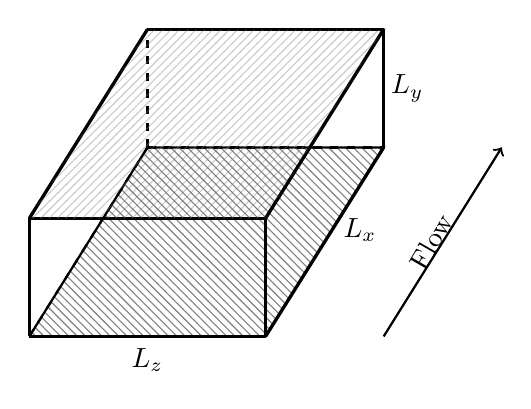
\begin{tikzpicture}[thick,scale=3]
    \coordinate (A1) at (0, 0);
    \coordinate (A2) at (0, 0.5);
    \coordinate (A3) at (1, 0.5);
    \coordinate (A4) at (1, 0);
    \coordinate (B1) at (0.5, 0.8);
    \coordinate (B2) at (0.5, 1.3);
    \coordinate (B3) at (1.5, 1.3);
    \coordinate (B4) at (1.5, 0.8);
    \draw[pattern=north west lines, pattern color=gray] (A1) -- (B1) -- (B4) -- (A4);
    \coordinate (AR1) at (1.5, 0);
    \coordinate (AR2) at (2, 0.8);

    \draw[very thick] (A1) -- (A2);
    \draw[very thick] (A2) -- (A3);
    \draw[very thick] (A3) -- (A4);
    \draw[very thick] (A4) -- (A1);

    \draw[dashed] (A1) -- (B1);
    \draw[dashed] (B1) -- (B2);
    \draw[very thick] (A2) -- (B2);
    \draw[very thick] (B2) -- (B3);
    \draw[very thick] (A3) -- (B3);
    \draw[very thick] (A4) -- (B4);
    \draw[very thick] (B4) -- (B3);
    \draw[dashed] (B1) -- (B4);
    \draw[->] (AR1) -- (AR2);

    %\draw[fill=black!20,opacity=0.5] (A1) -- (A2) -- (A3) -- (A4);
    %\draw[fill=red,opacity=0.6] (A1) -- (A2) -- (B2) -- (B1);
    %\draw[fill=black,opacity=0.6] (B1) -- (B2) -- (B3) -- (B4);
    %\draw[fill=blue,opacity=0.6] (A3) -- (B3) -- (B4) -- (A4);
    \draw[pattern=north east lines, pattern color=gray, opacity=0.4] (A2) -- (B2) -- (B3) -- (A3);
    \node[] at (0.5,-0.10) {$L_z$};
    \node[] at (1.4,0.45) {$L_x$};
    \node[] at (1.6,1.05) {$L_y$};
    \node[rotate=60] at (1.7,0.4) {Flow};
\end{tikzpicture}
   \includegraphics[width=10cm]{Figures/Domain.png}
    \caption{Schematic representation of simulation domain with an example pseudo-realistic surface mounted. Normalization of lengths with $H$ is applied in the figure.}
    \label{fig:domain}
\end{figure}
A number of DNS have been carried out in fully developed turbulent plane channels, in which the flow is driven by a constant pressure gradient.
A representation of the simulation domain is shown in figure~\ref{fig:domain}, where $x$, $y$ and $z$ denote streamwise, wall-normal and spanwise directions with respective velocity components $u$, $v$ and $w$.
The roughness are mounted on both upper wall and lower wall.
Channel half height, which is the distance between the deepest trough in roughness and the centre plane of the channel, is labeled as $H$ and will be used to normalize the geometrical scales.
The incompressible Navier-Stokes equations are solved using the pseudo-spectral solver SIMSON~\citep{Chevalier}, where wall-parallel directions are discretized in Fourier space, while in wall-normal direction Chebyshev discretization is employed.
Immersed Boundary Method (IBM) based on~\citet{goldstein93} is used to impose the no-slip boundary condition on the roughness by introducing an external volume force field directly to the Navier-Stokes equation.
The presently used IBM implementation has been validated and used in previous studies~\citep{PhysRevFluidsPourya,Vanderwel19,stroh_schaefer_frohnapfel_forooghi_2020}.\\
The Navier-Stokes equation writes
\begin{equation}
    \nabla\cdot \textbf{u}=0~,
\end{equation}
\begin{equation}
    \frac{\partial \textbf{u}}{\partial t}+\nabla\cdot(\textbf{uu})=-\frac{1}{\rho}\nabla p+\nu\nabla^2\textbf{u}-\frac{1}{\rho}P_x\hat{\mathbf{e_x}}+\textbf{f}_\text{IBM}~,
\end{equation}
where $\textbf{u}=(u,v,w)^\intercal$ is the velocity vector and $P_x$ is the mean pressure gradient in the flow direction added as a constant and uniform source term to the momentum equation to drive the flow in the channel. 
Here $p$, $\hat{\mathbf{e_x}}$, $\rho$, $\nu$ and $\textbf{f}_\text{IBM}$ are pressure fluctuation, streamwise basis vector, density, kinematic viscosity and external body force term due to IBM, respectively.
Periodic boundary conditions are applied in the streamwise and spanwise directions. 
No-slip boundary condition is applied on the rough walls.
The friction Reynolds number is defined as $Re_\tau=u_\tau(H-k_{\text{md}})/\nu$, where $u_\tau=\sqrt{\tau_w/\rho}$ and $\tau_w=-P_x\cdot (H-k_{\text{md}})$ are the friction velocity and wall shear stress, respectively. Melt-down height denoted by $k_{\text{md}}$ is the mean roughness height measured from the deepest trough. Note that we use $(H-k_{\text{md}})$ which is the mean half cross section area divided by the channel width -- or arguably the effective channel half height -- as the reference length scale in these definitions. In total, four different values of $Re_\tau$ in the range of 250-1000 are simulated in the present work in order to be able to cover different regimes. The simulations designed to study the effect of roughness topography are, however, performed mainly at $Re_\tau=500$.

The simulation domain is discretized in equidistant grid in wall-parallel directions while in wall-normal direction cosine stretching based on Chebyshev node distribution is applied.
The selection of grid size must take into consideration both flow and roughness length scales.
As reflected by ~\citet{BUSSE2015129}, each roughness wavelength should be represented by multiple computational cells.
Since we prescribe the PS in the roughness generation approach, the range of present roughness wavelengths can be prescribed.
Here the smallest roughness wavelength, labeled as $\lambda_1$, is the crucial quantity for horizontal grid resolution.
Therefore, in the view of the present computational capacity, $\lambda_1=0.08H$ is prescribed for the following simulations.
Mesh independence study is carried out, from which the smallest roughness wavelength being resolved by 8-10 cells in each directions is found adequate  to obtain the converged double averaged velocity profile.
Overall, the grid size $\Delta^+<5$ in wall-parallel directions is proven to be appropriate through the mesh independence test.
In wall-normal directions, cosine stretching mesh is adopted for the Chebychev discretization.
It is also checked through the mesh independence test that for present types of rough surfaces, a vertical cell number of 401 is sufficient in delivering a converged result at highest $Re_\tau\approx1000$, thanks to the overresolving of roughness structure by cosine stretching grid near wall.
\subsection{Description of cases}
\label{sec:cases}
%%%%%%%%%%%%%%%%%%%%%%%%%%%%%%%
\begin{figure}
    \centering
    \begin{subfigure}[t]{.49\linewidth}
    \centering
             \begin{tikzpicture}[]
        \centering
        \begin{axis}[
            ylabel={PDF},
            xlabel={k/H},
            ymax=0.05,
            width=.8\textwidth,
            height=.8\textwidth,
            legend style={font=\tiny,anchor=north west,fill=none},
            legend pos=north west,
            legend cell align={left},
            label style={font=\footnotesize},
            tick label style={font=\footnotesize}
            ]
            \addplot [
            black,solid,thick,
            ]
            table [x=X, y=Y,col sep=comma]{CSV/HPDG14F1.csv};
    \node[black,right] at (axis cs: -0.01,0.025) {$Sk=0.48$};
			\addplot [
            black,dashed,thick,
            ]
            table [x=X, y=Y,col sep=comma]{CSV/HPDN14F1.csv};
    \node[black] at (axis cs: 0.061,0.03) {$Sk=0$};
						\addplot [
            black,dotted,thick,
            ]
            table [x=X, y=Y,col sep=comma]{CSV/HPDP14F1.csv};
    \node[black,right] at (axis cs: 0.07,0.025) {$Sk=-0.48$};
        \end{axis}
        \end{tikzpicture}

    \caption{PDF of roughness.} %\\ \full: $Sk=0$, \dashed: $Sk=-0.48$, \dotted: $Sk=0.48$}
    \end{subfigure}\hfill%
    \begin{subfigure}[t]{.49\linewidth}
        \centering
    \begin{tikzpicture}
\begin{loglogaxis}[
		xlabel={$q/q_{\text{ref}}$},
		ylabel={$q_{\text{ref}}E_k(q)/k_{\text{rms}}^2$},
		xmin=0.1,xmax=100,
		ymin=0.000001,ymax=10,
		%ticks=none,
		clip=true,
		set layers,
		clip mode=individual,
		height=.8\textwidth,
		width=.8\textwidth,
        label style={font=\footnotesize},
        tick label style={font=\footnotesize}
		%axis line style={draw opacity=0}
		%xtick={0,800,...,2400},
		%colorbar,
		%point meta min=0,
		%point meta max=1.11,
		%colorbar style={
		%ytick={0,0.2,...,1.11}
		%}
	]
	\centering
\addplot [thick, color=blue, on layer=axis background]
graphics[xmin=0.1,ymin=0.000001,xmax=100,ymax=10]{Figures/PS_p.png};
    \draw[red,dashed,thick] (1,0.000001) -- (1,10);
    \draw[red,dashed,thick] (10,0.000001) -- (10,10);
    \node[label={[rotate=-90]{\scriptsize$\lambda=0.8H$}}] at (axis cs:1.05,0.5) {};
                \node[label={[rotate=-90]{\scriptsize$\lambda=0.08H$}}] at (axis cs:10.05,0.5) {};
    \draw[red] (1.3,0.08161) -- (1.803,0.08161);
    \draw[red] (1.803,0.05) -- (1.803,0.08161);                
        \node[black,right] at (axis cs: 1.803,0.07) {{\tiny $p=-2$}};
        
        \draw[red] (5.3,0.009) -- (9,.009);
    \draw[red] (9,0.009) -- (9,0.0056);                
        \node[black,right] at (axis cs: 9,0.007) {{\tiny $p=-1$}};
\end{loglogaxis}
\end{tikzpicture}
    \caption{Normalized PS density with different $p$.}
    \end{subfigure}
    \begin{subfigure}[t]{.49\linewidth}
        \centering
    \begin{tikzpicture}
\begin{loglogaxis}[
		xlabel={$q/q_{\text{ref}}$},
		ylabel={$q_{\text{ref}}E_k(q)/k_{\text{rms}}^2$},
		xmin=0.1,xmax=100,
		ymin=0.000001,ymax=10,
		%ticks=none,
		clip=true,
		set layers,
		clip mode=individual,
		height=.8\linewidth,
		width=.8\linewidth,
        label style={font=\footnotesize},
        tick label style={font=\footnotesize}
		%axis line style={draw opacity=0}
		%xtick={0,800,...,2400},
		%colorbar,
		%point meta min=0,
		%point meta max=1.11,
		%colorbar style={
		%ytick={0,0.2,...,1.11}
		%}
	]
	\centering
\addplot [thick, color=blue, on layer=axis background]
graphics[xmin=0.1,ymin=0.000001,xmax=100,ymax=10]{Figures/PS_l1.png};
    \draw[red,dashed,thick] (1,0.000001) -- (1,10);
    \draw[red,dashed,thick] (0.5,0.000001) -- (0.5,10);
    \draw[red,dashed,thick] (10,0.000001) -- (10,10);
    \node[label={[rotate=-90]{\scriptsize$\lambda=0.8H$}}] at (axis cs:1.05,0.5) {};
        \node[label={[rotate=-90]{\scriptsize$\lambda=1.6H$}}] at (axis cs:0.45,0.5) {};
                \node[label={[rotate=-90]{\scriptsize$\lambda=0.08H$}}] at (axis cs:10.05,0.5) {};
        \draw[red] (1.15,0.039) -- (1.803,0.039);
    \draw[red] (1.803,0.039) -- (1.803,0.025);                
        \node[black,right] at (axis cs: 1.803,0.047) {{\tiny $p=-1$}};
\end{loglogaxis}
\end{tikzpicture}
    \caption{Normalized PS density with different $\lambda_0$, $p=-1$.}
    \end{subfigure}\hfill%
    \begin{subfigure}[t]{.49\linewidth}
        \centering
    \input{tikz/PSforl2}
    \caption{Normalized PS density with different $\lambda_0$, $p=-2$.}
    \end{subfigure}
    \caption{Statistical representation of the studied Roughness-In (b,c,d) wavenumber $q$ is normalized by the reference wavenumber $q_{\text{ref}}=2\pi/(0.8H)$. Vertical dashed lines are high-pass filtering and low-pass filtering, corresponding to $\lambda_0$ \& $\lambda_1$ respectively. }%\color{red}scale with lambda1}
    \label{fig:HPDS}
\end{figure}
Using the roughness generation algorithm introduced in section \ref{sec:gen}, multiple samples are generated.
%Statistical properties are documented in table~\ref{tab:SumOfCase}.
In the present work, different types of PDF will be combined with power-law PS, that is $E_k(\textbf{q})=C_0(\norm{\textbf{q}}/q_0)^p$, where \textbf{q} is the wavenumber vector $\textbf{q}=(q_x,q_z)^\intercal$, $q_0=2\pi/\lambda_0$ is the smallest wavenumber corresponding to the largest in-plane length scale $\lambda_0$, $C_0$ is a constant to scale the roughness height, and $p$ is the spectral slope of the power-law PS.
The overview of the configurations of PDF and PS is illustrated in figure~\ref{fig:HPDS}.
In figure~\ref{fig:HPDS} (b,c,d) the PS density normalized by the r.m.s. of the roughness height are compared in pairs.
%As is shown, the configuration of the PS is characterized by a single parameter, namely the PS slope $p$. The upper and lower cut-off wavelengths of the PS are labeled as $\lambda_0$ and $\lambda_1$, respectively.
The upper and lower cutoff wavelength $\lambda_0$ and $\lambda_1$ are transformed to cutoff wavenumbers $q_0=2\pi/\lambda_0$ and $q_1=2\pi/\lambda_1$, which are represented by the red dashed lines in figure~\ref{fig:HPDS} (b,c,d) on the left and right side of the figures respectively.
As stated in the previous section, the lower cutoff wavelength is related to the grid resolution and a value of $\lambda_1=0.08H\approx8\Delta_{x}\approx8\Delta_{z}$ is applied for all roughness topographies in the present work. With an isotropic roughness and a fixed $\lambda_1$, the PS is determined by two remaining parameters, $\lambda_0$ and $p$.
In present work, two values of $p$ ($p=-1$ and $p=-2$) are examined, the PS of which are shown in figure~\ref{fig:HPDS} (b).
For the selection of $p$ values we seek similarity to previous works~\citep{anderson_meneveau_2011,BARROS20181,nikora2019}.
Moreover, two different upper cutoff wavelengths ($\lambda_0=0.8H$ and $\lambda_0=1.6H$) of the roughness PS are investigated. 
Power spectrum with $\lambda_0=0.8H$ and $1.6H$ with identical slopes $p$ are compared in figure~\ref{fig:HPDS}(c,d), where wavenumber $q$ is normalized by referencing wavenumber $q_{\text{ref}}=2\pi/(0.8H)$

Three types of PDFs with positive, zero and negative skewness are examined in the present work.
Covering a relatively large range of $Sk$ is intended to ensure that the results can be generalized to a wide spectrum of naturally occurring roughness in different applications.
The non-skewed roughness is described by a Gaussian distribution. %which writes
%\begin{equation}
%    f(k|\mu,\sigma)=\frac{1}{\sqrt{2\pi\sigma^2}}\text{exp}\bigl(-\frac{(k-\mu)^2}{%2\sigma^2}\bigl)~,
%\end{equation}
%where $\mu$ and $\sigma$ are mean value and standard deviation respectively.
For the positively skewed roughness, Weibull distribution is used, which writes
%\begin{equation}
%    f(k)=\lambda_s^c c k^{c-1}\text{exp}(-(\lambda_s k)^c)~,
%\end{equation}
%where $\frac{1}{\lambda_s}$ and $c$ are scale and shape parameter respectively.
%The value of $\lambda_s$ and $c$ are adjusted to meet identical $Ku$ value with Gaussian distribution, i.e. $Ku\approx3$, while $Sk$ of which is adjusted to reach 0.48.
\begin{equation}
f(k)= K \beta^K k^{(K-1)}e^{-(\beta k)^K}~,
\end{equation}
\begin{figure}
\centering
\begin{subfigure}{.47\linewidth}
\input{tikz/N14.tikz}
%\caption{$N14$}
\end{subfigure}
\hfill
\begin{subfigure}{.47\linewidth}

\input{tikz/N24.tikz}
%\vspace{-0.5cm}
%\caption{$N24$}
\end{subfigure}
\begin{subfigure}{.47\linewidth}
\input{tikz/N18.tikz}
%\caption{$N18$}
\end{subfigure}
\hfill
\begin{subfigure}{.47\linewidth}

\input{tikz/N28.tikz}
%\vspace{-0.5cm}
%\caption{$N28$}
\end{subfigure}

\begin{subfigure}{.47\linewidth}
\begin{tikzpicture}
\pgfplotsset{
    scale only axis,
}
\begin{axis}[
		%xlabel={$L_x/H$},
		ylabel={$z/H$},
		ylabel shift = 3.5 pt,
		xmin=0,xmax=2.4,
		ymin=0,ymax=0.8,
		unit vector ratio=1 1 1,
		y dir=reverse,
		clip=true,
		set layers,
		clip mode=individual,
		width=.75\linewidth,
		xtick={0,0.6,...,2.4},
		ytick={0,0.4,...,0.8},
		label style={font=\footnotesize},
		tick label style={font=\footnotesize},
%				colorbar,
%		point meta min=0.0,
%		point meta max=0.1227,
%		colorbar style={
%%				xlabel={$k/H$},
%%				xlabel shift = 10.5 pt,
%		ytick={0,0.12},
%		width=0.2cm
%		}
	]
	\centering
\addplot [thick, color=blue, on layer=axis background]
graphics[xmin=0,ymin=0,xmax=2.4,ymax=0.8]{Figures/G14c.png};
    \draw[red,dashed,thick] (0,0.4) -- (2.4,0.4);
    \node[black,right] at (axis cs: 0,0.65) {\contour{black}{(e) $G14$}};
\end{axis}
\begin{axis}[
		%xlabel=$L_x [H]$,
		ylabel={$k/H$},
		xmin=0,xmax=2.4,
		ymin=0,ymax=0.12,
		%y dir=reverse,
		clip=true,
		set layers,
		clip mode=individual,
	    height=0.05\linewidth,
		width=.75\linewidth,
		axis x line*=bottom,
		axis y line*=left,
		xticklabels=\empty,
		ytick={0.12},
		label style={font=\footnotesize},
		yticklabel style={/pgf/number format/fixed},
		tick label style={font=\footnotesize},
		at={(0,0.28\linewidth)}
	]
	\centering
    \addplot+[ name path=A,
            red,solid,thick,mark=none
            ]
            table [x=X, y=Y,col sep=comma]{CSV/G14H.csv};
    \path[name path=B,black,mark=none] (axis cs:0,0) -- (axis cs:2.4,0);
    \addplot[gray,mark=none] fill between[of=A and B];
\end{axis}
\end{tikzpicture}
%\caption{$G14$}
\end{subfigure}
\hfill
\begin{subfigure}{.47\linewidth}

\input{tikz/G24.tikz}
%\vspace{-0.5cm}

%\caption{$G24$}
\end{subfigure}
\begin{subfigure}{.47\linewidth}
\input{tikz/G18.tikz}

%\caption{$G18$}
\end{subfigure}
\hfill
\begin{subfigure}{.47\linewidth}
\input{tikz/G28.tikz}
%\vspace{-0.5cm}
%\caption{$G28$}
\end{subfigure}
\begin{subfigure}{.47\linewidth}
\input{tikz/P14.tikz}
%\caption{$P14$}
\end{subfigure}
\hfill
\begin{subfigure}{.47\linewidth}
\input{tikz/P24.tikz}
%\vspace{-0.5cm}
%\caption{$P24$}
\end{subfigure}
\begin{subfigure}{.47\linewidth}
\input{tikz/P18.tikz}
%\caption{$P18$}
\end{subfigure}
\hfill
\begin{subfigure}{.47\linewidth}
\input{tikz/P28.tikz}
%\vspace{-0.5cm}
%\caption{$P28$}
\end{subfigure}
\caption{Roughness maps with configuration $M1-500$, color indicates height. 1D roughness profile at $z=0.4H$ (\Rdashed{}) is shown above each roughness map. (a-d): negatively skewed, (e-h): zero skewness, (i-l): positively skewed; left column: $p=-1$. right column, $p=-2$.}
\label{AllPM1}
\end{figure}
where the parameters $K$ and $\beta$ can be used to adjust the standard deviation and skewness of the distribution. The skewness is always adjusted to the value of 0.48. Similar to the Gaussian distribution the Kurtosis of the Weibull distribution is always equal to three.
A negatively skewed PDF is obtained by flipping the PDF of a positively skewed Weibull PDF. Here $Sk=-0.48$ is prescribed. In the present work, the $99\%$ confidence interval of roughness height PDF, $k_{99}$, is used as the characteristic size of roughness, i.e. $k=k_{99}$. This measure is related to the standard deviation of the roughness, and hence can be directly prescribed. We used a fixed value of $k=0.1H$ in all cases. Indeed, $k$ is a statistical measure of maximum peak-to-trough roughness size, which unlike the absolute peak-to-trough size $k_\text{t}$, is not deteriorated by extreme events.
These types of PDFs are illustrated in figure~\ref{fig:HPDS}.
Moreover, in order to avoid extreme high roughness elevations in the simulations, roughness heights outside 1.2 times the $99\%$ confidence interval of PDF are excluded.
Therefore, the peak-to-trough height $k_\text{t}=0.12H$ for all roughness in the present work.
Combining the three types of PDF (with different values of $Sk$) with four types of PS (two values of $p$ and $\lambda_0$ each) twelve different roughness topographies are studied in the present work, which are summarized in table \ref{tab:SumOfCase}.
Selected patches of all 12 roughness topographies % corresponding to size configuration $M1-500$, i.e. 
on surfaces with size $2.4H \times 0.8H$, are displayed in figure~\ref{AllPM1}.
Above each roughness map, the 1D roughness profile at $z=0.4H$ along streamwise direction is shown.
%In figure~\ref{AllPM1}(a-d), the roughness topographies with $Sk=-0.48$ are shown.
%The major part of the surface is higher than its median height.
%The negative skewness can be denoted as 'pit-dominant'. %, where degradation of the surface shows in the form of indentation.
%Topographies with $Sk=0.48$ are shown in figure~\ref{AllPM1}(i-l), where a large portion of the height function is concentrated under the median height.
%Thus, the roughness can be regarded as 'peak-dominant' with strong protrusion into the fluid.
%However, In figure~\ref{AllPM1}(e-h), the height probability distribution obeys Gaussian distribution where both pits and peaks are shown. 
%Therefore, the majority of the surface elevation is centering around the median height.

%On the left column of figure~\ref{AllPM1}, roughness topographies with PS slope $p=-1$ are shown, while on the right column $p=-2$ are shown.
%From both 2D roughness map and 1D roughness profile, one can observe that the roughness structures with $p=-1$ have smaller length scale.
%From the PS in figure\ref{fig:HPDS}(b) one can see that the relative smaller wavelengths of roughness contain more power in rough surfaces with $p=-1$, while for $p=-2$  larger wavelengths of roughness are emphasized.
%To parameterize the spatial distribution of roughness elements, $ES$ is introduced as a measure of roughness density %($ES=2\Lambda$, where $\Lambda$ is the density factor~\citep{Rij}).
%As can be seen in table~\ref{tab:SumOfCase}, strong correlation is observed between the PS slope $p$ and $ES$, i.e. $ES$ increases with decreasing $p$~\citep{Stewart2019}.

For each roughness sample, simulations in full-span and minimal channels are carried out. For minimal channels the spanwise size $L_z$ is the main subject of the study. 
As the log-layer flow structures are set by the spanwise dimension $L_z$~\citep{Flores2010}, it is often most critical in terms of reducing the computational cost.
%However, one obstacle in reducing the spanwise extent of channel is the largest presenting wavelength in spanwise direction $\lambda_0$.
%In order to discuss further possibilities in reducing the channel width, a minimal channels with $L_z=0.5\lambda_0$ are employed.
The spanwise size of the present minimal channels are designed to fulfil the three criteria set by inequality (\ref{MINI2}). The first criterion ($L_z^+>100$) stems from the fact that the computational domain must accommodate the near wall cycle of turbulence and, unlike the other two criteria, is independent of the roughness topography. The second criterion ($L_z^+\geq\tilde{k}^+/0.4$) ensures that roughness can be included in 'healthy turbulent' zone under critical height.
%the entire wall-normal extent of the roughness {\color{red}sublayer} remains below the critical height, i.e. within the `healthy turbulence' zone.
We translate the criteria for a realistic roughness by replacing $\tilde{k}$ for the sinusoidal roughness by the characteristic roughness height $k$ for any arbitrary roughness. 
%{\color{red}Referring to the second criteria from inequality (\ref{MINI2}) that the entire wall-normal extent of the roughness remains below the critical height, We further expand the critical height above roughness sub-layer $y_r\approx0.5\lambda_0$.
%Therefore, the second criteria writes $$L_z\geq1.25\lambda_0.$$}
The third criterion states that the minimal channel should contain the roughness wavelength.
However, for the realistic surfaces a single characteristic wavelength is not naturally determined.
A conservative choice for this limit of the channel width can be the largest in-plane length scale, which is $\lambda_0$ in the present study. This ensures that all wavelengths present in the roughness topography are included in the spanwise domain.
Recalling the aim of reducing the roughness simulation cost, however, we seek a less conservative choice, in which some of the larger wavelengths are excluded.
Particularly, for simulations of engineering roughness, it is often impractical to include extremely large roughness scales. %since their contribute insignificant effect to the flow.
To formalize our choice, we denote the largest spanwise wavelength that a domain can accommodate as $\lambda^*$, and calculate the portion of surface energy that larger wavelengths contribute to the original roughness as
\begin{equation}
\Phi\left(\frac{2\pi}{\lambda^*}\right)=\frac{\int_{2\pi/\lambda_0}^{2\pi/\lambda^*}E_k(q)\mathrm{d}q}{\int_{2\pi/\lambda_0}^{2\pi/\lambda_1}E_k(q)\mathrm{d}q}~.
\end{equation}
where $\lambda$ is the discrete wavelength. 
If the spanwise domain size is $\lambda^*$, the simulation resolves a roughness with $1-\Phi$ portion of the original surface variance.

In the current research we examine a choice of spanwise channel size corresponding to half the size of the largest length scale, i.e. $\lambda_0/2$. With the adopted power-law PS, it leads to the values of $1-\Phi$ equal or larger than 90\% for all samples under investigation.
Hence the third criterion is replaced by $L_z\geq\lambda_{1/2}$, where $\lambda_{1/2}=\lambda_0/2$, which means that the simulations resolve at least 90\% of the original surface variance.
The new criterion leads to a minimum channel width of $L_z=0.8H$ for half of the investigated roughness topographies (those with $\lambda_0=1.6H$) and $L_z=0.4H$ for the other half (those with $\lambda_0=0.8H$).
%With such domain setup, the spanwise wavelength in minimal channel is constrained to $\lambda_1\leq\lambda\leq\lambda_{1/2}$ due to the limited channel width, while the streamwise roughness scale doesn't suffer from the truncated channel size. 
We label the minimal channels with the former (larger) and latter (smaller) spanwise sizes as $M$1 and $M$2, respectively.
For roughness samples with $\lambda_0=0.8H$ simulations at both $M$1 and $M$2 channels are carried out. %to investigate any effect of the channel spanwise size, especially in $M$1 channel due to the doubled spanwise width relative to $M$2, the largest spanwise wavelength equals to the largest in-plane length scale $\lambda_0=0.8H$, thus the effect of truncation by $\lambda_{1/2}$ in spanwise direction can be investigated.
To complete the investigation, some simulation with a further reduced channel size $M$3 ($L_z=0.3H$) are carried out. % $\Phi(2\pi/(0.3H))=18\%$    roughness topography $G24$ (the case abbreviation system will be declared in following text).
%Without complicating the structure of the simulation cases, topography $G28$ whose $\lambda_0=1.6H$ is simulated in further reduced computational domain, $M$2, where $L_z=0.4H$ with $\Phi(2\pi/(0.4H)=16\%$.
It is worth mentioning that, since $k=0.1H$ holds for all topographies, $M$1, $M2$ and $M$3 channels fulfill the $L_z\geq k/0.4$ criterion. For all simulation configurations the streamwise channel size $L_x$ is set according to the equation \ref{MINI1} once $L_z$ is known.
%\begin{figure}
    %\centering
       %         \begin{tikzpicture}[]
        \centering
        \begin{axis}[
            ylabel={$qE_k(q)/\int E_k(q)\mathrm{d}q$},
            xlabel={$q/q_{ref}$},
            ymin=-0.000001, ymax=0.000023,
			%xmin=1,xmax=500,
            width=0.7\textwidth,
            height=0.7\textwidth,
			xmode=log,
            legend style={font=\tiny,anchor=north west},
            legend pos= north west,
            label style={font=\footnotesize},
            tick label style={font=\footnotesize}
            ]
						\addplot [
            red,solid,thick,mark=*,only marks,
            ]
            table [x=X, y=Y,col sep=comma]{CSV/PSQ1-81.csv};
            \addlegendentry{$p=-1$, $\lambda_0=0.8H$}
						\addplot [
            blue,solid,thick,mark=*,only marks,
            ]
            table [x=X, y=Y,col sep=comma]{CSV/PSQ2-81.csv};
            \addlegendentry{$p=-2$, $\lambda_0=0.8H$}
                        \addplot [
            red,dashed,thick,
            ]
            coordinates{
            (5.2418, -0.0001)
            (5.2418, 0.0001)
            };
            \addlegendentry{$\Bar{\lambda}=0.1459$}
                                    \addplot [
            blue,dashed,thick,
            ]
            coordinates{
            (3.1457, -0.0001)
            (3.1457, 0.0001)
            };
            \addlegendentry{$\Bar{\lambda}=0.2096$}
            \addplot [
            black,dashed,thick,
            ]
            coordinates{
            (2, -0.0001)
            (2, 0.0001)
            };
            \addlegendentry{$\lambda_{1/2}$}
        \end{axis}
        \end{tikzpicture}

   %\caption{Normalized premultiplied PS of surfaces with $\lambda_0=0.8H$, $p=-1$ and $p=-2$ as a function of wavenumber $q$. Mean wavelength $\Bar{\lambda}$ are marked with vertical dashed lines with corresponding color, black dashed line represents $\lambda_{1/2}$}
   %\label{PSQ18}
%\end{figure}



%One must, however, note that replacing $k_{sine}$ with $k$ this is a rather liberal interpretation of the original criterion since the peak-to-trough size of a sinusoidal roughness is indeed equal to $2 k_{sine}$. Hence a more conservative condition for the 

%As one of the major objectives of this work, the application of minimal channel is examined.
%To investigate the characteristics of minimal channels, two sizes of minimal channels are employed.
%Since the critical length scale of a minimal channel is the spanwise width of the channel, $L_z$, which determines the turbulence scale or the critical height $y_c$, the minimal channel is labeled in terms of its spanwise width $L_z$.
%The channel spanwise width is set according to the criteria Eqn.~\ref{MINI2}.
%Following the criteria, the spanwise widths of minimal channels are selected according to the $\lambda_0$, i.e. $L_z=0.4H$ (labeled as $M2$) and $L_z=0.8H$ (labeled as $M1$) for the roughness topographies with $\lambda_0=0.4H$ and $\lambda_0=0.8H$ respectively.
%The corresponding streamwise extent of minimal channels are prescribed according to Eqn.~\ref{MINI1}.
%Have to mention that due to the relative larger upper cutoff wavelength for the topography with $\lambda_0=0.8H$, only the minimal channel $M1$ with $L_z=0.8H$ is suitable to properly resolve the roughness structure.
%However for the roughness topographies with $\lambda_0=0.4H$, $M1$ will be employed additionally in order to acquire a deeper understanding of minimal channel mechanism.
%To evaluate the capability of minimal channels, conventional full span channel simulations, labeled as $F$, with size $L_x\times L_y\times L_z=8H\times2H\times4H$ are also carried out for comparison.
%However due to the unfeasible computational cost for carrying out DNS at high Reynolds number for each of the rough surfaces shown above, an exemplary roughness corresponding to roughness configuration $G24$ is selected.
%The simulation configurations of the cases are summarized in Table~\ref{tab:Re}.
%Consistent spanwise width is chosen for $M2$s and $M1$s at different $Re_\tau$.
%The selection of channel length is according to Eqn.~\ref{MINI1}, due to the different settings of $Re_\tau$ the lengths of the channels are varied.
%Have to mention that due to the excessive heavy simulation task brought by the full size simulations at $Re_\tau=750\&1000$, the biggest channel size is reduced in a minimal channel fashion, which is considered as pseudo-full channel and labeled as $M0$.\\

Simulations are carried out at four different friction Reynolds numbers Re$_\tau=250$, $500$, $750$ and $1000$, at fixed $k/H=0.1$, leading to $k^+=25$, $50$, $75$, and $100$. However the parametric study on roughness topography is only conducted at $k^+=50$. Apart from minimal channel simulations, conventional full span channel simulations with the size $L_x\times L_y\times L_z=8H\times2H\times4H$, labeled as $F$, are also carried out for all roughness topographies. For the two highest Reynolds numbers, however, such large simulations are costly. Consequently, for these Reynolds numbers, the largest investigated channels are smaller than the $F$ channel (but still larger than $M$1/$M$2/$M$3). These channels are labeled as $M$0. Table \ref{tab:Re} summarizes the details of all simulations carried out for rough channels. In order to provide a reference for determining the roughness function $\Delta U^+$, additional smooth-wall simulations are also performed in $M2$, $M1$ and $F$-sized channels at Re$_\tau=500$ (not shown in the table). Overall, each rough-wall simulation case is defined by a combination of roughness topography and simulation configuration (channel size and Reynolds number). Throughout the article, the following naming convention is used to describe the cases: 
\begin{equation}
    \overbrace{\underbrace{\boxed{\;G\;}}_\text{PDF}\;\;\underbrace{\boxed{ \;2\;}}_\text{$-p$} \underbrace{\boxed{\;4\;}}_\text{\;$10\lambda_{1/2}/H$}}^{\text{Topography}}\;|\overbrace{\underbrace{\boxed{\;F\;}}_{\text{ch. size}}- \underbrace{\boxed{500}}_{10k^+}}^{\text{Simulation configuration}}~.
\end{equation}
\begin{itemize}
    \item The first character indicates the type of PDF; $G$ for Gaussian distribution, $P$ for positively skewed ($Sk\approx0.48$), and $N$ for negatively skewed ($Sk\approx-0.48$).
    \item The second digit indicates the PS spectral slope; $1$ for $p=-1$ and $2$ for $p=-2$.
    \item The third digit represents the half of large cutoff wavelength $\lambda_{1/2}$, with which channel width is determined; $4$ for $\lambda_{1/2}=0.4H$ and $8$ for $\lambda_{1/2}=0.8H$.
    \item The following character(s) indicates the channel spanwise size; $F$ for full channel ($L_z=4H$), $M$1 and $M$2 for the larger ($L_z=0.8H$) and the smaller ($L_z=0.4H$) minimal channels, respectively. $M$3 utilizes the spanwise width $L_z=0.3H$.
    $M$0 is introduced to the cases which $k^+=75$ and $100$ with $L_z=2H$ and $1H$, respectively
    \item The last number denotes $10k^+$, or equivalently, $Re_\tau$.
\end{itemize}
%In figure~\ref{AllNM1}, figure~\ref{AllGM1} and figure~\ref{AllPM1} roughness maps in minimal channels $M1-500$ i.e. surfaces with size $2.4H \times 0.8H$ are shown.\\


    \begin{table}
        \centering
        \begin{tabular}{cccccccccc}
            Topography & $Sk$ & $p$ & $\lambda_0/H$&$k_\text{a}/H$&$k_{\text{md}}/H$&$k_{\text{rms}}/H$&$L_x^{\text{corr}}/H$&$S_f/S$&ES$_x$\\[3pt]
            $P14$ & $0.48$ & $-1$ & 0.8&0.017&0.046&0.0208&0.050&0.28&0.57\\
            $P18$ & $0.48$ & $-1$ & 1.6&0.017&0.046&0.0208&0.054&0.27&0.54\\
            $P24$ & $0.48$ & $-2 $& 0.8&0.017&0.046&0.0208&0.104&0.21&0.44\\
            $P28$ & $0.48$ & $-2 $& 1.6&0.017&0.046&0.0208&0.170&0.19&0.39\\[3pt]
            $G14$ & $0$ & $-1$ & 0.8&0.016&0.061&0.0200&0.050&0.27&0.54\\
            $G18$ & $0$ &$ -1$ & 1.6&0.016&0.061&0.0200&0.054&0.26&0.53\\
            $G24$ & $0$ & $-2$ & 0.8&0.016&0.061&0.0200&0.104&0.20&0.43\\
            $G28$ & $0$ & $-2$ & 1.6&0.016&0.061&0.0200&0.168&0.18&0.37\\[3pt]
            $N14$ & $-0.48$ & $-1$ & 0.8&0.017&0.074&0.0208&0.050&0.28&0.57\\
            $N18$ & $-0.48$ & $-1$ & 1.6&0.017&0.074&0.0208&0.054&0.27&0.54\\
            $N24$ & $-0.48$ & $-2$ & 0.8&0.017&0.074&0.0208&0.104&0.21&0.44\\
            $N28$ & $-0.48$ & $-2$ & 1.6&0.017&0.074&0.0208&0.170&0.19&0.39\\
        \end{tabular}
                \caption{Roughness topographical properties, where 
        $Sk=(1/k_{\text{rms}}^3)\int_S(k-k_{\text{md}})^3\mathrm{d}S$, $k_\text{a}=(1/S)\int_S|k-k_{\text{md}}|\mathrm{d}S$ is the mean absolute height deviation from the melt-down height $k_{\text{md}}=(1/S)\int_Sk\mathrm{d}S$ measured from deepest trough. $k_{\text{rms}}=\sqrt{(1/S)\int_S(k-k_{\text{md}})^2\mathrm{d}S}$ is the standard deviation of the height function. $S_f$ is the  total frontal projected area of the roughness. $L_x^{\text{corr}}$ refers to the length scale where the roughness auto-correlation in streamwise direction drops under 0.2. $\text{ES}=(1/S)\int_S|\partial k/\partial x|\mathrm{d}S$ represents the effective slope.}
        \label{tab:SumOfCase}
    \end{table}
%     \begin{adjustbox}{width=\textwidth,center}
    % \begin{adjustbox}{center}   


   %     \begin{tabular}{ c c c c c c c }
%             Topographies & $Re_\tau$ & $L_x(H)$ & $L_z(H)$& $Nx$ & $Nz$& configuration \\   %             \hline
%            \multirow{3}{*}{all} & \multirow{3}{*}{250} & \multicolumn{1}{c}{4} & %\multicolumn{1}{c}{0.4}& \multicolumn{1}{c}{216} & %\multicolumn{1}{c}{24}&\multicolumn{1}{c}{$M2-250$} \\
%            
%                                 & \multicolumn{1}{c}{5} & \multicolumn{1}{c}{0.8}&  %\multicolumn{1}{c}{384} & \multicolumn{1}{c}{72}& \multicolumn{1}{c}{$M1-250$} \\
%                                 
%                                 & \multicolumn{1}{c}{8} & \multicolumn{1}{c}{4}  &  %\multicolumn{1}{c}{480} & \multicolumn{1}{c}{240} &\multicolumn{1}{c}{$F-250$}\\
%                                 \hline
%            \multirow{3}{*}{all} & \multirow{3}{*}{250} & \multicolumn{1}{c}{2.0} & %\multicolumn{1}{c}{0.4}& \multicolumn{1}{c}{256} & %\multicolumn{1}{c}{96}&\multicolumn{1}{c}{$M2-500$} \\
%            
%                                 & \multicolumn{1}{c}{2.4} & \multicolumn{1}{c}{0.8}& %\multicolumn{1}{c}{256} & \multicolumn{1}{c}{96}& \multicolumn{1}{c}{$M1-500$} \\
%                                 
%                                 & \multicolumn{1}{c}{8} & \multicolumn{1}{c}{4}  &  %\multicolumn{1}{c}{900} & \multicolumn{1}{c}{480} &\multicolumn{1}{c}{$F-500$}\\
%                                 \hline
%             \multirow{3}{*}{all} &\multirow{3}{*}{250} & \multicolumn{1}{c}{1.4} & %\multicolumn{1}{c}{0.4}& \multicolumn{1}{c}{288} & \multicolumn{1}{c}{96}& %\multicolumn{1}{c}{$M2-750$} \\
%             
%                                 & \multicolumn{1}{c}{2.4} & \multicolumn{1}{c}{0.8}&  %\multicolumn{1}{c}{480} & \multicolumn{1}{c}{160}& \multicolumn{1}{c}{$M1-750$} \\
%                                 
%                                 & \multicolumn{1}{c}{4} & \multicolumn{1}{c}{2}  &  %\multicolumn{1}{c}{640} & \multicolumn{1}{c}{320} &\multicolumn{1}{c}{$M0-750$}\\
%                                 \hline
%            \multirow{3}{*}{all} &\multirow{3}{*}{250} & \multicolumn{1}{c}{1.2} & %\multicolumn{1}{c}{0.4}& \multicolumn{1}{c}{288} & \multicolumn{1}{c}{96}& %\multicolumn{1}{c}{$M2-1000$} \\
%                                 & \multicolumn{1}{c}{2.4} & \multicolumn{1}{c}{0.8}&  %\multicolumn{1}{c}{576} & \multicolumn{1}{c}{192}& \multicolumn{1}{c}{$M1-1000$} \\
%                                 & \multicolumn{1}{c}{3} & \multicolumn{1}{c}{1}  &  %\multicolumn{1}{c}{720} & \multicolumn{1}{c}{240}& \multicolumn{1}{c}{$M0-1000$} \\%

%        \end{tabular}
\begin{table}
    \centering

    \begin{tabular}{ccccccccccc}
         Topographies&Configuration&$Re_\tau$&$L_x/H$&$L_z/H$&$N_x$&$N_z$&$\Delta_x^+$&$\Delta_z^+$&$\Delta_{y,k}^+$ & FTT \\[3pt]
         $G24$&$M2-250$&250&4.0&0.4&512&48&1.95&2.08&0.88&1200\\
         $G24$&$M1-250$&250&5.0&0.8&576&96&2.17&2.08&0.88&300\\
         $G24$&$F-250$&250&8.0&4.0&900&480&2.22&2.08&0.88&100\\[3pt]
         $G24$&$M3-500$&500&2.0&0.3&256&48&3.91&3.13&1.74&1000\\
         $**4$ \& $G28$&$M2-500$&500&2.0&0.4&256&48&3.91&4.17&1.74&2000\\
         all&$M1-500$&500&2.4&0.8&256&96&4.69&4.17&1.74&500\\
         all&$F-500$&500&8.0&4.0&900&480&4.44&4.17&1.74&80\\[3pt]
         $G24$&$M2-750$&750&1.4&0.4&288&96&3.65&3.13&2.59&1200\\
         $G24$&$M1-750$&750&2.4&0.8&480&160&3.75&3.75&2.59&300\\
         $G24$&$M0-750$&750&4.0&2.0&640&320&4.69&4.69&2.59&100\\[3pt]
         $G24$&$M2-1000$&1000&1.2&0.4&288&96&4.17&4.17&3.53&500\\
         $G24$&$M1-1000$&1000&2.4&0.8&576&192&4.17&4.17&3.53&300\\
         $G24$&$M0-1000$&1000&3.0&1.0&720&240&4.17&4.17&3.53&100\\
    \end{tabular}
            \caption{Summary of all simulation cases including roughness topography and simulation configurations. For all cases $L_y/H=2$,$N_y=401$. Moreover, $**4$ indicates all roughness topographies with $\lambda_{1/2}=0.4H$, $\Delta_{y,k}^+$ indicates the grid size at the roughness height i.e. $y=0.1H$, flow through time (FTT$=TU_b/L_x$) for statistics collection duration are shown in the last column, where $T$ is the total integral time, $U_b=(1/H_{\text{eff}})\int_0^{H}U\mathrm{d}y$ is the bulk velocity, $H_{\text{eff}}=H-k_{\text{md}}$.}
            \label{tab:Re}
\end{table}

%\begin{figure}
%\centering
%        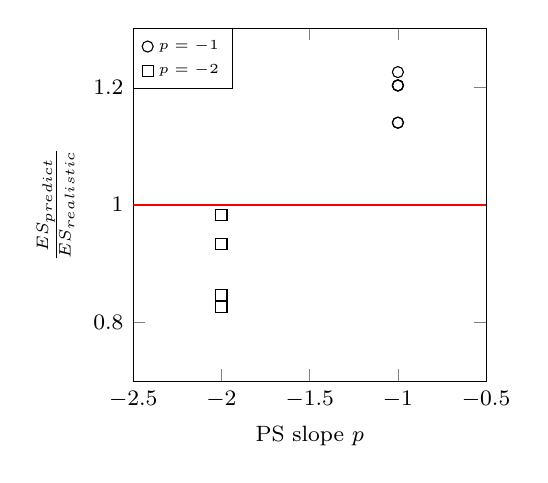
\begin{tikzpicture}[]
        \centering
        \begin{axis}[
            ylabel={$\frac{ES_{predict}}{ES_{realistic}}$},
            xlabel={PS slope $p$},
            ymin=0.7, ymax=1.3,
			xmax=-0.5,
			xmin=-2.5,
			%xtick={-2,-1.5,...,-0.4},
            width=.5\linewidth,
            height=.5\linewidth,
            label style={font=\footnotesize},
			legend style={font=\tiny,at={(0,1)},anchor=north west},
            tick label style={font=\footnotesize}
            ]
			\addplot [
            black,only marks,mark=o,
            ]
            coordinates{
            (-1,1.1394)
            (-1,1.2027)
            (-1,1.2027)
            (-1,1.2254)
            (-1,1.1394)
            (-1,1.2027)
            };
            			\addlegendentry{$p=-1$}
            			\addplot [
            black,only marks,mark=square,
            ]
            coordinates{
            (-2,0.8265)
            (-2,0.9324)
            (-2,0.8456)
            (-2,0.9828)
            (-2,0.8265)
            (-2,0.9324)
            };
            			\addlegendentry{$p=-2$}
			% \fill[color=green!40,opacity=40] (0,1.05) -- (9,1.05) -- (9,0.95) -- (0,0.95) -- cycle;
			 			%\fill[color=yellow!40,opacity=40] (0,0.18) -- (9,9.18) -- (9,8.82) -- (0,-0.18) -- cycle;
						\addplot [
            red,thick,solid,mark=square,
            ]
            coordinates{
            (-3, 1)
            (0, 1)
            };
			%\node[red,right] at (axis cs: 7.8,7.5) {\tiny $\pm5\%$};
        \end{axis}
        \end{tikzpicture}
%    \caption{ESvsp}
%\caption{Assessment of ES correlation as a function of PS slope $p$}
%    \label{EScorr}
%\end{figure}

\subsection{Post-processing}
\label{sec:post}
%%%%%
The time-averaged flow field over a rough surface is heterogeneous in horizontal directions.
In order to analyze the one-dimensional mean profile of the flow, we apply double averaging, as proposed by~\citet{SHAW198251}.
The double-averaged velocity profile in the wall-normal direction $\bigl<\overline{u}\bigr>(y)$ is obtained by averaging the time-averaged velocity over wall-parallel directions, i.e.
\begin{equation}
    \bigl<\overline{u}\bigr>(y)=\frac{1}{S}\iint_S\overline{u}(x,y,z)\mathrm{d}x\mathrm{d}z~.
\end{equation}
where $\overline{u}(x,y,z)$ is time averaged streamwise velocity, $S$ is the wall-normal projected plan area (i.e. area of the corresponding smooth wall) and angular bracket $\bigl<\cdot\bigr>$ denotes horizontal averaging.
The double-averaged velocity profile $\bigl<\overline{u}\bigr>(y)$ will be denoted as $U$ for simplicity.
The time-averaged velocity field is obtained over a long enough period of time.
%It should be mentioned relatively longer simulation averaging time (in terms of flow through time) are applied for collection of minimal channel statistics due to the bursting effect~\cite{Flores2010}.
A minimum of 300 flow-through-times is used for the statistical integration in minimal channels due to the bursting effect~\citep{Flores2010}.
Initial transients are removed from the statistical integration.
%The statistics is tested for convergence.

The influence of roughness on the mean flow is a downward shift in the inner-scaled streamwise velocity profile relative to the smooth case~\citep{Schultz2009}.
In other words, as a result of the outer layer similarity~\citep{Townsend}, which states that outer-layer flow is unaffected by the near wall events except for the effect due to the wall shear stress, the downward shift of the velocity profile is approximately a constant value in the logarithmic region and possibly beyond if the outer-flow geometry and Reynolds number are matched.
This downward velocity shift in the logarithmic region is referred to as roughness function~\citep{CLAUSER19561,hama1954} $\Delta U^+$. Introducing the roughness function to the logarithmic law of the wall (log-law hereafter), it writes
\begin{equation}
        U^+=\frac{1}{\kappa}\text{ln}(y^+-d^+)+B-\Delta U^+~.
\end{equation}
where $\kappa\approx0.4$ is the von Kármán constant, $\textit{B}\approx5.2$ is the log-law intercept for the smooth wall, $d$ indicates the zero plane displacement which will be talked in detail in the following section, and the superscript $+$ indicates scaling in wall units.
Based on the pioneering work by~\citet{Nikuradse1933}, the roughness function in the fully rough regime is a sole function of the inner-scaled roughness size $k_s^+$ for the sand-grain roughness according to
\begin{equation}
    \Delta U^+ =B-8.48+\frac{1}{\kappa}\text{ln}(k_s^+)~.
    \label{asysptot}
\end{equation}
Equation~\ref{asysptot} is the basis for the definition of `equivalent' sand-grain roughness (also denoted by $k_s$) for an arbitrary roughness with the same roughness function.

%Considering the crucial importance of roughness function $\Delta U^+$, the central interested value of this paper is thus the downward shift of the velocity profile induced by the rough wall relative to a smooth wall.
In the present work, the roughness function $\Delta U^+$ is calculated as the mean offset of the inner-scaled mean velocity profile over the logarithmic layer for the cases with $Re_\tau\approx500$.
Since corresponding smooth channels in $M2$, $M1$ and $F$ with matched $Re_\tau\approx500$ are available, this quantity is calculated by direct comparison to the smooth case.
For those cases with varied $Re_\tau$,  further smooth channel simulations with matched $Re_\tau$ are required in order to derive the corresponding profile shift, which causes unfavourable computational effort. 
Having in mind that log-law applies for minimal smooth channels under critical height $y_c$, a good approximation of velocity profile in log region of the smooth channels can be drawn from the log-law, thus $\Delta U^+$ is estimated by the velocity shift at the critical height $y_c^+=0.4\times L_z^+$ relative to the log-law $U^+=(1/\kappa)\text{ln}(y^+)+5.2$, where $\kappa=0.4$.

%The calculation of $\Delta U^+$ is validated in minimal channels with $k^+=25-100$ by comparing smooth channel simulation results with the results derived from log-law, the averaged error of $\Delta U^+$ over all tested $k^+$ is lower than 3\%.\\
Finally it must be noted that, unlike a smooth channel, the origin of the wall-normal coordinate for the log-law is not naturally defined for a rough wall.
In this regard, \citet{jackson_1981} suggested use of moment centroid of the drag profile on rough surface as the virtual origin for the logarithmic velocity profile.
The definition of the virtual wall zero-plane displacement $d$ in present work follows Jackson's method.

\section{Results}
\label{DNS}
\subsection{Evaluation of minimal-channel simulations}
\label{sec:EMC}
In order to assess the applicability of the minimal channel, the simulations of the roughness topography $G24$ with variation of channel size and $k^+$ are analyzed. 
The comparison of different channel sizes at matched $k^+\approx50$, i.e. the cases  $G24M3-500$, $G24M2-500$, $G24M1-500$ and $G24F-500$, is discussed in \cref{width}. This is followed by the results for all different roughness topographies in \cref{minimal channel-roughness topography}.
As mentioned before, the roughness generation process in the present research has a random nature, and only statistical properties can be prescribed. To assess the effect of this randomness eight independent simulations are carried out for eight random realizations of the roughness topography $G24$ with $k^+\approx50$. The results are presented in~\cref{Rando}.
Finally in \cref{Res}, one roughness topography is studied in a wide range of roughness Reynolds numbers ($k^+=25-100$) in order to assess the prediction of the minimal channel in different rough regimes. Here the roughness topography $G24$ is evaluated using minimal channels $M$2 and $M$1 and (pseudo) full-span channels $F/M$0. 
\subsubsection{Minimal channels with different spanwise sizes}
\label{width}
\begin{figure}
\centering
\begin{subfigure}[t]{.42\linewidth}
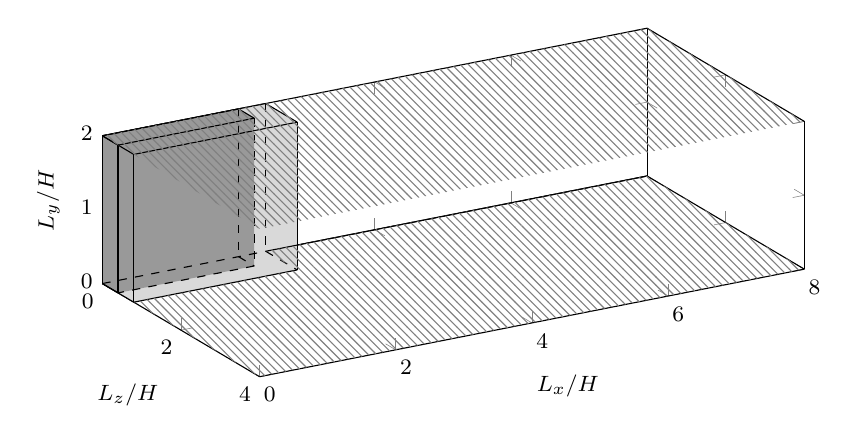
\begin{tikzpicture}
\pgfplotsset{
    scale only axis,
}
\begin{axis}[
view={-30}{20},
		xlabel={$L_x/H$},
		ylabel={$L_z/H$},
		zlabel={$L_y/H$},
		unit vector ratio=1 1 1,
		xmin=0,xmax=8,
		ymin=0,ymax=4,
		zmin=0,zmax=2,
		y dir=reverse,
		clip=true,
		set layers,
		clip mode=individual,
		height=.7\textwidth,
		width=.9\textwidth,
		xtick={0,2,...,8},
		ytick={0,2,...,4},
		ztick={0,1,2},
		label style={font=\footnotesize},
		tick label style={font=\footnotesize},
	]
	\pgfmathparse{atan(tan(-50)*sin(70))}
  \let\a=\pgfmathresult
  \pgfmathparse{atan(tan(90+50)*sin(70))}
  \let\b=\pgfmathresult  

	\centering
%\addplot3 [thick, color=blue, on layer=axis background]
%graphics[xmin=0,ymin=0,xmax=8,ymax=4,zmin=0,zmax=0]{Figures/G24Fc.png};

\fill[color=gray!30,opacity=100] (0,0.8,0) -- (2.4,0.8,0) -- (2.4,0.8,2) -- (0,0.8,2) -- cycle;
\fill[color=gray!30,opacity=100] (0,0,0) -- (0,0.8,0) -- (0,0.8,2) -- (0,0,2) -- cycle;
\fill[color=gray!30,opacity=100] (0,0,2) -- (0,0.8,2) -- (2.4,0.8,2) -- (2.4,0,2) -- cycle;
\fill[color=gray!80,opacity=100] (0,0.4,0) -- (2,0.4,0) -- (2,0.4,2) -- (0,0.4,2) -- cycle;
\fill[color=gray!80,opacity=100] (0,0,0) -- (0,0.4,0) -- (0,0.4,2) -- (0,0,2) -- cycle;
\fill[color=gray!80,opacity=100] (0,0,2) -- (0,0.4,2) -- (2,0.4,2) -- (2,0,2) -- cycle;
\draw[-,black] (2.4,0,0) -- (8,0,0);

%\draw[-,black] (0,0,0) -- (2,0,0);
\draw[-,dashed,black] (2,0,0) -- (2,0.4,0);
\draw[-,dashed,black] (2,0.4,0) -- (0,0.4,0);
\draw[-,black] (0,0.4,0) -- (0,0,0);


\draw[-,black] (0,0,2) -- (2,0,2);
\draw[-,black] (2,0,2) -- (2,0.4,2);
\draw[-,black] (2,0.4,2) -- (0,0.4,2);
\draw[-,black] (0,0.4,2) -- (0,0,2);

\draw[-,black] (0,0,2) -- (0,0,0);
\draw[-,dashed,black] (2,0,2) -- (2,0,0);
\draw[-,dashed,black] (2.4,0,2) -- (2.4,0,0);
\draw[-,black] (2.4,0.8,2) -- (2.4,0.8,0);
\draw[-,dashed,black] (2,0.4,2) -- (2,0.4,0);
\draw[-,black] (0,0.4,2) -- (0,0.4,0);
\draw[-,black] (0,0.8,2) -- (0,0.8,0);

\draw[-,dashed,black] (0,0,0) -- (2.4,0,0);
\draw[-,dashed,black] (2.4,0,0) -- (2.4,0.8,0);
\draw[-,black] (2.4,0.8,0) -- (0,0.8,0);
\draw[-,black] (0,0.8,0) -- (0,0,0);


\draw[-,black] (0,0,2) -- (2.4,0,2);
\draw[-,black] (2.4,0,2) -- (2.4,0.8,2);
\draw[-,black] (2.4,0.8,2) -- (0,0.8,2);
\draw[-,black] (0,0.8,2) -- (0,0,2);

\fill[pattern=north west lines, pattern color=gray] (0,0.8,0) -- (8,0.8,0) -- (8,4,0) -- (0,4,0) -- cycle;
\fill[pattern=north west lines, pattern color=gray] (2.4,0,0) -- (8,0,0) -- (8,0.8,0) -- (2.4,0.8,0) -- cycle;
\fill[pattern=north west lines, pattern color=gray] (0,0,2) -- (8,0,2) -- (8,4,2) -- (0,4,2) -- cycle;
%graphics[xmin=0,ymin=0,xmax=8,ymax=4,zmin=0,zmax=0]{Figures/G24Fc.png};
%\node[gray,left] at (axis cs: 2,0.2,0) {\tiny$M2$};
%\node[gray,left] at (axis cs: 2.4,0.6,0) {\tiny$M1$};
%\node[gray,left] at (axis cs: 8,3.8,0) {\tiny$F$};
\end{axis}
\end{tikzpicture}
\caption{Schematic simulation domain of $F-500$, $M1-500$ and $M2-500$, hatch pattern represents roughness.}
\end{subfigure}\hfill
\begin{subfigure}[t]{.57\linewidth}
\begin{tikzpicture}
\pgfplotsset{
    scale only axis,
}
\begin{axis}[
		xlabel={$L_x/H$},
		ylabel={$L_z/H$},
		unit vector ratio=1 1 1,
		xmin=0,xmax=8,
		ymin=0,ymax=4,
		y dir=reverse,
		clip=true,
		set layers,
		clip mode=individual,
		width=.7\textwidth,
		xtick={0,2,...,8},
		ytick={0,2,...,4},
		label style={font=\footnotesize},
		tick label style={font=\footnotesize},
		colorbar,
		point meta min=0,
		point meta max=0.1226,
		colorbar style={
			xlabel={$k/H$},
			xlabel shift = 10.5 pt,
		ytick={0,0.12},
		width=0.2cm
		}
	]
	\centering
\addplot [thick, color=blue, on layer=axis background]
graphics[xmin=0,ymin=0,xmax=8,ymax=4]{Figures/G24Fc.png};
\draw[color=black,thick] (0, 0) rectangle (2, 0.4);
\draw[color=black,thick] (0, 0) rectangle (2.4, 0.8);
\node[black,left] at (axis cs: 2,0.2) {\textbf{$M$2-500}};
\node[black,left] at (axis cs: 2.4,0.6) {\textbf{$M$1-500}};
\node[black,left] at (axis cs: 8,3.8) {\textbf{$F$-500}};
\end{axis}
\end{tikzpicture}
\caption{Roughness map of $G24F-500$}
\end{subfigure}
\caption {Comparison of channel sizes, black frames indicate minimal channels $M1-500$ \& $M2-500$}
\label{G24F}
\end{figure}
\begin{figure}
	\begin{subfigure}[t]{.49\textwidth}
	\centering
	        \begin{tikzpicture}[]
        \centering
        \begin{axis}[
            ylabel={$U^+$},
            xlabel={$(y-d)^+$},
            ymin=0, ymax=30,
			xmin=1,xmax=500,
            width=1.05\textwidth,
            height=0.8\textwidth,
			xmode=log,
            legend style={fill=white,font=\tiny,anchor=north west},
            legend pos=north west,
            label style={font=\footnotesize},
            tick label style={font=\footnotesize}
            ]
            \addplot [
            black,dashed,thick,
            ]
            table [x=X, y=Y,col sep=comma]{CSV/UprofileG24FM1.csv};
            \addlegendentry{critical height $y_c$}
            			            \addplot [
            gray!50,solid,thick,
            ]
            table [x=X, y=Y,col sep=comma]{CSV/G24M31.csv};
            \addlegendentry{$G24M3-500$}
			            \addplot [
            red,solid,thick,
            ]
            table [x=X, y=Y,col sep=comma]{CSV/UprofileG24FM6.csv};
            \addlegendentry{$G24M2-500$}
			\addplot [
            green,solid,thick,
            ]
            table [x=X, y=Y,col sep=comma]{CSV/UprofileG24FM7.csv};
            \addlegendentry{$G24M1-500$}
						\addplot [
            blue,solid,thick,
            ]
            table [x=X, y=Y,col sep=comma]{CSV/UprofileG24FM8.csv};
            \addlegendentry{$G24F-500$}
						\addplot [
            black,dashdotted,thick,
            ]
            table [x=X, y=Y,col sep=comma]{CSV/UprofileG24FM9.csv};
            \addlegendentry{$U^+=(\frac{1}{0.4})\text{log}(y^+)+5.2$}
            \draw [dashdotted,red, thick] (50-45.80,0) -- (50-45.80,30);
            \addplot [
            black,dashed,thick,
            ]
            table [x=X, y=Y,col sep=comma]{CSV/UprofileG24FM2.csv};
            \addplot [
            blue,dashed,thick,
            ]
            table [x=X, y=Y,col sep=comma]{CSV/UprofileG24FM3.csv};
            \addplot [
            green,dashed,thick,
            ]
            table [x=X, y=Y,col sep=comma]{CSV/UprofileG24FM4.csv};	            
\addplot [
            red,dashed,thick,
            ]
            table [x=X, y=Y,col sep=comma]{CSV/UprofileG24FM5.csv};
\draw [dashed,gray!50] (60,0) -- (60,30);

        \end{axis}
        \end{tikzpicture}
	\caption{Mean velocity profile. (\full: Rough, \dashed: Smooth)}
	\end{subfigure}\hfill
	\begin{subfigure}[t]{.49\textwidth}
	\centering
	        \begin{tikzpicture}[]
        \centering
        \begin{axis}[
            ylabel={$\Delta U^+$},
            xlabel={$(y-d)^+$},
            ymin=-2, ymax=8,
			xmin=1,xmax=500,
            width=1.05\textwidth,
            height=0.8\textwidth,
			xmode=log,
            legend style={font=\tiny,anchor=south east},
            legend pos= south east,
            label style={font=\footnotesize},
            tick label style={font=\footnotesize}
            ]
            \addplot [
            black,dashed,thick,
            ]
            coordinates{
            (160, 10)
            (160, -5)
            };
            \addlegendentry{critical height $y_c$}
						\addplot [
            red,solid,thick,
            ]
            table [x=X, y=Y,col sep=comma]{CSV/DUprofileG24mf23.csv};
            \addlegendentry{$G24M2-500$}
									\addplot [
            green,solid,thick,
            ]
            table [x=X, y=Y,col sep=comma]{CSV/DUprofileG24mf24.csv};
            \addlegendentry{$G24M1-500$}
						\addplot [
            blue,solid,thick,
            ]
            table [x=X, y=Y,col sep=comma]{CSV/DUprofileG24mf25.csv};
            \addlegendentry{$G24F-500$}
                        \draw [dashdotted,red, thick] (50-45.80,-8) -- (50-45.80,30);
            \addplot [
            black,dashed,thick,
            ]
            coordinates{
            (80, 10)
            (80, -5)
            };


        \end{axis}
        \end{tikzpicture}
	\caption{Velocity offset profile.}
	\end{subfigure}
\caption{Simulation results of roughness type $G24$. Gray: $M3-500$, red: $M2-500$, green: $M1-500$, blue: $F-500$. Red vertical line indicates roughness height measures from the zero-plane displacement $(k-d)^+$.}
\label{UG24}
\end{figure}
The 3D schematic representations of minimal channels $M2$ and $M1$ as well as the full span channel $F$ used for simulations at $k^+\approx 50$ are shown in figure~\ref{G24F}(a); $M3$ is not shown for simplicity.
The hatched pattern indicates where the roughness is mounted.
Roughness topography $G24$ in the full-size simulation is shown in figure~\ref{G24F}(b). 
For a direct comparison, boundaries of minimal channels $M1$ and $M2$ are represented by the black frames.
The pseudo-random surfaces for each configuration is generated independently.
That is, for a specific topography, the surface height map in each simulation is unique, but they all share identical statistical properties.

The inner-scaled velocity profiles obtained from roughness topography configuration $G24$ with $k^+\approx50$ are shown in figure~\ref{UG24}(a). 
Colored dashed lines are the velocity profiles extracted from smooth channel. 
The color indicates the size of channel.
The critical heights of minimal channels $M2-500$ and $M1-500$, i.e. $y_c^+=0.4\times L_z^+=80\text{ and }160$ are illustrated by black vertical dashed lines in the figure, respectively.
While the critical height of $M3-500$ i.e. $y_c^+=60$ is shown with gray vertical dashed line. It can be observed from the figure, that minimal channel cases $M2-500$ and $M1-500$ successfully reproduce the velocity profile of a conventional full-span channel under the critical height $y_c$. 
The velocity profiles deviate above the critical height $y_c$ due to the nature of minimal channels.
For $G24M3-500$, however, some discrepancy of the profile can be observed even under its critical height.
In figure~\ref{UG24}(b), the velocity offset profiles for $F$, $M1$ and $M2$ channels are displayed. The velocity offset profiles are obtained by subtracting the rough channel velocity profile from each corresponding smooth channel velocity profiles.
The velocity offset profile from minimal channels $M1$, $M2$ and full-span channel on the right panel show excellent agreement.
%One should recall that for this topography, minimal channel $M2$ has a spanwise size $L_z=\lambda_{1/2}=\lambda_0/2$, where $\lambda_{1/2}$ is the length scale below which 90\% of the surface elevation variance resides, i.e. $\Phi(2\pi/\lambda_{1/2})<10\%$.
Consequently, it seems like the velocity offset is not meaningfully affected by absence of the large wavelengths in spanwise direction with small contribution to the roughness height power spectrum.
This however does not hold for channel $M3$ where $\Phi(2\pi/L_z)=18\%$. A similar parameter study performed for roughness topography $G28$ (not shown here) revealed that the velocity offset starts to deviate for channel $M2$ ($\Phi(2\pi/L_z)=16\%$). In both cases the deviation of the velocity profiles starts when the contribution of excluded large wavelengths in the roughness height spectrum is larger than 10\%.

It is observed that due to the outer layer similarity the velocity offset in logarithmic layer reaches approximately a constant value.
%The value of roughness function $\Delta U^+$ can thus be evaluated by averaging the velocity offset in logarithmic layer.
In the present work, $\Delta U^+$ of minimal channels is obtained by averaging the mean velocity offset from each critical height $y_c^+$ to the half of channel half-height $0.5H^+$, while full span channels is averaged in the region $y+=80-250$.
This gives $\Delta U^+=6.3$ for case $G24F-500$ and $\Delta U^+=6.4$ and $6.2$ for cases $G24M1-500$ and $G24M2-500$, respectively.

\subsubsection{Minimal channels for different roughness topographies}
\label{minimal channel-roughness topography}
\begin{table}
\centering
    \begin{tabular}{c| c c c| c c c}
    & & $\Delta U^+$& & & $d/k$&\\[3pt]
     Case&$F-500$&$M1-500$&$M2-500$&$F-500$&$M1-500$&$M2-500$\\[3pt]
    $P14$&7.33&7.28&\textbf{7.35}&0.81&0.81&\textbf{0.82}\\
    $P24$&6.99&6.86&\textbf{6.92}&0.78&0.77&\textbf{0.80}\\
    $P18$&7.23&\textbf{7.34}&-&0.81&\textbf{0.81}&-\\
    $P28$&6.57&\textbf{6.87}&-&0.76&\textbf{0.76}&-\\[3pt]
     $G14$&6.67&6.66&\textbf{6.56}&0.95&0.94&\textbf{0.95}\\
     $G24$&6.30&6.39&$\textbf{6.43}^*$&0.92&0.90&$\textbf{0.92}^*$\\ 
    $G18$&6.56&\textbf{6.59}&-&0.95&\textbf{0.95}&-\\
    $G28$&5.94&\textbf{5.88}&-&0.90&\textbf{0.90}&-\\[3pt]
    $N14$&6.14&6.07&\textbf{5.87}&1.06&1.06&\textbf{1.06}\\
    $N24$&5.82&5.63&\textbf{5.80}&1.03&1.03&\textbf{1.05}\\
    $N18$&6.09&\textbf{6.06}&-&1.06&\textbf{1.06}&-\\
    $N28$&5.51&\textbf{5.58}&-&1.01&\textbf{1.02}&-\\
    \end{tabular}
    \caption{Summary of roughness function $\Delta U^+$ (left) and zero plane displacement $d/k$ (right) at $k^+\approx50$, bold values are taken as the minimal channel results. $^*$: mean value over 8 independent $G24M2-500$s}
\label{ResultAll}
\end{table}
Applying the same analysis to all topographies at $k^+\approx50$, roughness function $\Delta U^+$ are calculated and listed in table~\ref{ResultAll}.
It has to be mentioned that for case $G24M2-500$, multiple simulations are carried out for the purpose that will be discussed in~\cref{Rando}.
Therefore, roughness function of $G24M2-500$ is the mean roughness function $\overline{\Delta U^+}$ over $G24M2-500$s and marked with $^*$.
The value of $\Delta U^+$ predicted by minimal channels are compared with the prediction by full-span channels with matched topographical property in figure~\ref{DUfullmini}.
In this plot, the $\pm5\%$ disagreement interval is illustrated by the green shadow around $\Delta U_{\text{Mini}}^+/\Delta U_{\text{Full}}^+=1$ (red line).
Another key quantity widely discussed in the framework of roughness studies is the zero-plane displacement $d$. Similar to $\Delta U^+$, $d$ is often used as input to roughness models, and therefore, its prediction is of practical value. Motivated by that, in this section we also discuss predictions of $d$ by minimal channels.
The value of $d/k$ are also exhibited in the Table~\ref{ResultAll}.
Predicted zero-plane displacements $d$ in minimal channels are compared with full span channels in figure~\ref{DFullmini}.
It can be observed that minimal channel predictions show excellent agreement with conventional full span channel, the discrepancy lies under 5\%.
Consistent predictions of roughness function $\Delta U^+$ indicate %that with matched roughness statistical properties but unmatched surface height functions, i.e. those random surfaces sharing identical PS and PDF, the hydrodynamic property of roughness can be uniquely determined.
%At the same time,
the capability of the minimal channels in reproducing roughness function $\Delta U^+$ of the irregular pseudo-realistic roughness.%s is also demonstrated.\\
%\begin{table}[ht]
%\centering
%\caption{Summary of zero-plane displacement $d^+$ at $Re_\tau\approx500$, bold values are taken as the minimal channel results. $^*$: Mean value over 8 independent $G24M2-500$s}
%\begin{ruledtabular}
%    \begin{tabular}{c c c c}
%     Case&$F-500$&$M1-500$&$M2-500$\\
%     \hline
%    $P14$&40.74&40.38&\textbf{40.87}\\
%    $P24$&39.03&38.50&\textbf{40.02}\\
%    $P18$&40.52&\textbf{40.62}&-\\
%%    $P28$&37.80&\textbf{38.02}&-\\
 %    $G14$&47.33&47.17&\textbf{47.47}\\
%     $G24$&45.80&45.12&$\textbf{45.80}^*$\\ 
%    $G18$&47.25&\textbf{47.29}&-\\
%    $G28$&44.90&\textbf{44.82}&-\\
%    $N14$&53.10&53.11&\textbf{53.23}\\
%    $N24$&51.48&51.39&\textbf{52.45}\\
%    $N18$&52.83&\textbf{53.03}&-\\
%    $N28$&50.63&\textbf{50.38}&-\\
%    \end{tabular}
%    \end{ruledtabular}
%\label{ResultAlld}
%\end{table}
%\begin{figure}[ht]
%%    \centering
%    \begin{subfigure}[t]{.6\linewidth}
%            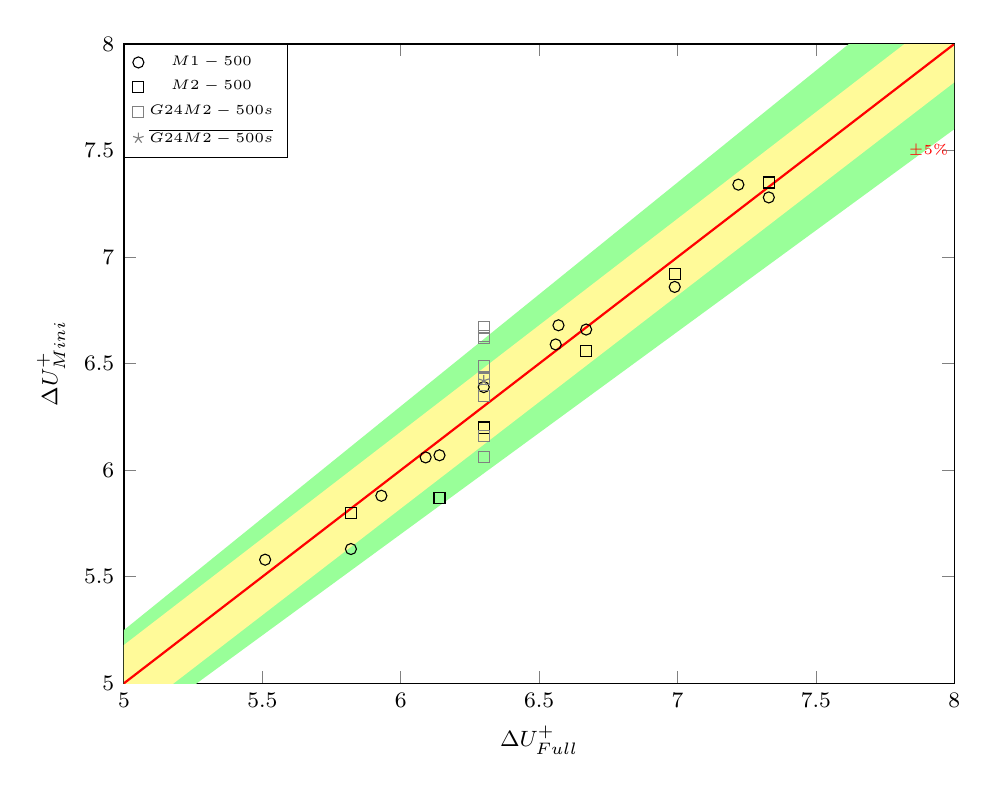
\begin{tikzpicture}[]
        \centering
        \begin{axis}[
            ylabel={$\Delta U_{Mini}^+$},
            xlabel={$\Delta U_{Full}^+$},
            ymin=5, ymax=8,
			xmax=8,
			xmin=5,
			%xtick={-2,-1.5,...,-0.4},
            width=1\linewidth,
            height=.8\linewidth,
            label style={font=\footnotesize},
			legend style={font=\tiny,at={(0,1)},anchor=north west},
            tick label style={font=\footnotesize}
            ]
			\addplot [
            black,only marks,mark=o,
            ]
            coordinates{
            (6.67, 6.66)
            (6.56, 6.59)
            (6.30,6.39)
            (5.93,5.88)
            (7.33,7.28)
            (7.22,7.34)
            (6.99,6.86)
            (6.57,6.68)
            (6.14,6.07)
            (6.09,6.06)
            (5.82,5.63)
            (5.51,5.58)
            };
			\addlegendentry{$M1-500$}
			\addplot [
            black,only marks,mark=square,
            ]
            coordinates{
            (6.67, 6.56)
            (6.30, 6.20)
            (7.33,7.35)
            (6.99,6.92)
            (6.14,5.87)
            (5.82,5.80)
            };
			\addlegendentry{$M2-500$}
						\addplot [
            gray,only marks,mark=square,
            ]
            coordinates{
            (6.30, 6.06)
            (6.30, 6.43)
            (6.30, 6.35)
            (6.30, 6.49)
            (6.30, 6.62)
            (6.30, 6.67)
            (6.30, 6.63)
            (6.30, 6.16)
            };
			\addlegendentry{$G24M2-500s$}
									\addplot [
            gray,only marks,mark=star,
            ]
            coordinates{
            (6.30, 6.42)
            };
			\addlegendentry{$\overline{G24M2-500s}$}
			 \fill[color=green!40,opacity=40] (0,0) -- (9,9.45) -- (9,8.55) -- cycle;
			 			\fill[color=yellow!40,opacity=40] (0,0.18) -- (9,9.18) -- (9,8.82) -- (0,-0.18) -- cycle;
						\addplot [
            red,thick,solid,mark=square,
            ]
            coordinates{
            (0, 0)
            (9, 9)
            };
			\node[red,right] at (axis cs: 7.8,7.5) {\tiny $\pm5\%$};
        \end{axis}
        \end{tikzpicture}
%    \end{subfigure}
%    \caption{$\Delta U^+$ predicted by minimal channels %against prediction by full span channel at $Re_\tau\approx500$, $\circ$: minimal channel $M1-500$, $\square$: minimal channel $M2-500$, {\color{gray}$\square$}: minimal channel of specific topography $G24M2-500$, {\color{gray}$\star$}: averaged $\Delta U^+$ over all $G24M2-500$s. Green shadow indicates prediction error interval of $\pm5\%$ around $\Delta U_{Full}^+=\Delta U_{Mini}^+$ (\Rfull). Yellow region represents the 95\% confidence interval basing on the analysis of $G24M2-500$s}
    %\label{DUfullmini}
%\end{figure}
\begin{figure}
    \centering
            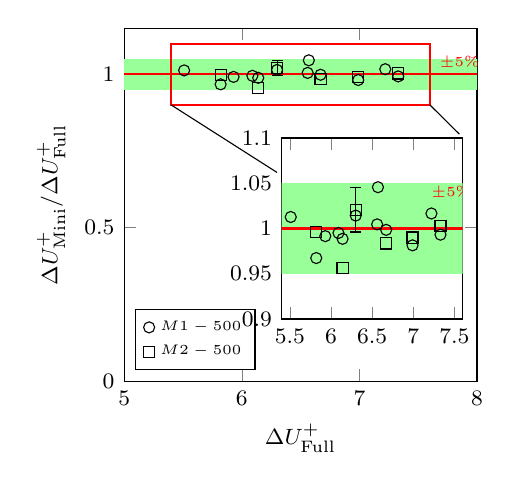
\begin{tikzpicture}[]
        \centering
        \begin{axis}[
            ylabel={$\Delta U_{\text{Mini}}^+/\Delta U_{\text{Full}}^+$},
            xlabel={$\Delta U_{\text{Full}}^+$},
            ymin=0, %ymax=1.2,
			xmax=8,
			xmin=5,
			%xtick={-2,-1.5,...,-0.4},
            width=.5\linewidth,
            height=.5\linewidth,
            label style={font=\footnotesize},
            legend style={font=\tiny,anchor=south west},
                        legend pos=south west,
            tick label style={font=\footnotesize}
            ]
			\addplot [
            black,only marks,mark=o,
            ]
            coordinates{
            (6.67,6.66/6.67)
            (6.56,6.59/6.56)
            (6.30,6.39/6.30)
            (5.93,5.88/5.93)
            (7.33,7.28/7.33)
            (7.22,7.34/7.22)
            (6.99,6.86/6.99)
            (6.57,6.87/6.57)
            (6.14,6.07/6.14)
            (6.09,6.06/6.09)
            (5.82,5.63/5.82)
            (5.51,5.58/5.51)
            };
			\addlegendentry{$M1-500$}
			\addplot [
            black,only marks,mark=square,
            ]
            coordinates{
            (6.67, 6.56/6.67)
            (6.30, 6.43/6.30)
            (7.33,7.35/7.33)
            (6.99,6.92/6.99)
            (6.14,5.87/6.14)
            (5.82,5.80/5.82)
            };
			\addlegendentry{$M2-500$}%
			

%						\addplot [
%            gray,only marks,mark=square,
%            ]
%            coordinates{
%            (6.30, 6.46/6.30)
%            (6.30, 6.42/6.30)
%            (6.30, 6.56/6.30)
%            (6.30, 6.58/6.30)
%            (6.30, 6.58/6.30)
%            (6.30, 6.19/6.30)
%            (6.30, 6.54/6.30)
%            (6.30, 6.30/6.30)
%            };
%			\addlegendentry{$G24M2-500s$}
			 \fill[color=green!40,opacity=40] (0,1.05) -- (9,1.05) -- (9,0.95) -- (0,0.95) -- cycle;
			 			%\fill[color=yellow!40,opacity=40] (0,0.18) -- (9,9.18) -- (9,8.82) -- (0,-0.18) -- cycle;
			 		
						\addplot [
            red,thick,solid,mark=square,
            ]
            coordinates{
            (0, 1)
            (9, 1)
            };
            \draw[color=red,thick] (5.4, 0.9) rectangle (7.6, 1.1);
			\node[red,right] at (axis cs: 7.6,1.04) {\tiny $\pm5\%$};
						\addplot[
        only marks,
        mark=square,
        black,
        error bars/.cd, y dir=both, y explicit,
    ] plot coordinates {
                    (6.30, 6.43/6.30)+=(0, 0.1539/6.30) -=(0, 0.1539/6.30)
    };
        \coordinate (AR1) at (5.4, 0.9);
        \coordinate (AR2) at (6.3, 0.68);
        \coordinate (AR3) at (7.6, 0.9);
        \coordinate (AR4) at (7.85, 0.805);
         \draw[-] (AR1) -- (AR2);
         \draw[-] (AR3) -- (AR4);
        \end{axis}
        
                \begin{axis}[
            %ylabel={$\frac{\Delta U_{Mini}^+}{\Delta U_{Full}^+}$},
            %xlabel={$\Delta U_{Full}^+$},
            ymin=0.9,ymax=1.1,
			xmax=7.6,
			xmin=5.4,
			%xtick={-2,-1.5,...,-0.4},
            width=.32\linewidth,
            height=.32\linewidth,
            label style={font=\footnotesize},
            tick label style={font=\footnotesize},
            at={(0.165\linewidth,0.065\linewidth)}
            ]
			\addplot [
            black,only marks,mark=o,
            ]
            coordinates{
            (6.67,6.66/6.67)
            (6.56,6.59/6.56)
            (6.30,6.39/6.30)
            (5.93,5.88/5.93)
            (7.33,7.28/7.33)
            (7.22,7.34/7.22)
            (6.99,6.86/6.99)
            (6.57,6.87/6.57)
            (6.14,6.07/6.14)
            (6.09,6.06/6.09)
            (5.82,5.63/5.82)
            (5.51,5.58/5.51)
            };
			\addplot [
            black,only marks,mark=square,
            ]
            coordinates{
            (6.67, 6.56/6.67)
            (6.30, 6.43/6.30)
            (7.33,7.35/7.33)
            (6.99,6.92/6.99)
            (6.14,5.87/6.14)
            (5.82,5.80/5.82)
            };
%						\addplot [
%            gray,only marks,mark=square,
%            ]
%            coordinates{
%%            (6.30, 6.46/6.30)
 %           (6.30, 6.42/6.30)
 %           (6.30, 6.56/6.30)
 %           (6.30, 6.58/6.30)
 %           (6.30, 6.58/6.30)
 %           (6.30, 6.19/6.30)
 %           (6.30, 6.54/6.30)
 %           (6.30, 6.30/6.30)
 %           };

			 \fill[color=green!40,opacity=40] (0,1.05) -- (9,1.05) -- (9,0.95) -- (0,0.95) -- cycle;
			 			%\fill[color=yellow!40,opacity=40] (0,0.18) -- (9,9.18) -- (9,8.82) -- (0,-0.18) -- cycle;
						\addplot [
            red,thick,solid,mark=square,
            ]
            coordinates{
            (0, 1)
            (9, 1)
            };
			\node[red,right] at (axis cs: 7.1,1.04) {\tiny $\pm5\%$};
						 						\addplot[
        only marks,
        mark=square,
        black,
        error bars/.cd, y dir=both, y explicit,
    ] plot coordinates {
                    (6.30, 6.43/6.30)+=(0, 0.1539/6.30) -=(0, 0.1539/6.30)
    };
        \end{axis}
        \end{tikzpicture}
    \caption{Roughness function predicted by minimal channels $\Delta U^+_{\text{Mini}}$ normalized with full span channel prediction $\Delta U^+_{\text{Full}}$, $\circ$: $M1-500$, $\square$: $M2-500$. Green shadow indicates prediction error interval of $\pm5\%$ around $\Delta U_{\text{Mini}}^+/\Delta U_{\text{Full}}^+=1$ (\Rfull). $99\%$ confidence interval is shown for case $G24M2-500$}
    \label{DUfullmini}
\end{figure}
\begin{figure}
    \centering
            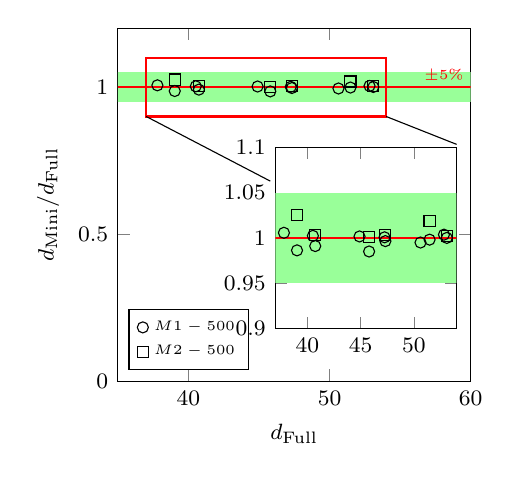
\begin{tikzpicture}[]
        \centering
        \begin{axis}[
            ylabel={$d_{\text{Mini}}/d_{\text{Full}}$},
            xlabel={$d_{\text{Full}}$},
            ymin=0, ymax=1.2,
			xmax=60,
			xmin=35,
			%xtick={-2,-1.5,...,-0.4},
            width=.5\linewidth,
            height=.5\linewidth,
            label style={font=\footnotesize},
            legend style={font=\tiny,anchor=south west},
                        legend pos=south west,
            tick label style={font=\footnotesize}
            ]
			\addplot [
            black,only marks,mark=o,
            ]
            coordinates{
            (40.74,40.38/40.74)
            (39.03,38.50/39.03)
            (40.52,40.62/40.52)
            (37.80,38.02/37.80)
            (47.33,47.17/47.33)
            (45.80,45.12/45.80)
            (47.25,47.29/47.25)
            (44.90,44.90/44.82)
            (53.10,53.11/53.10)
            (51.48,51.39/51.48)
            (52.83,53.03/52.83)
            (50.63,50.38/50.63)
            };
			\addlegendentry{$M1-500$}
			\addplot [
            black,only marks,mark=square,
            ]
            coordinates{
            (40.74, 40.87/40.74)
            (39.03, 40.02/39.03)
            (47.33,47.47/47.33)
            (45.80,45.84/45.80)
            (53.10,53.23/53.10)
            (51.48,52.45/51.48)
            };
			\addlegendentry{$M2-500$}
	
			 \fill[color=green!40,opacity=40] (0,1.05) -- (70,1.05) -- (70,0.95) -- (0,0.95) -- cycle;
			 			%\fill[color=yellow!40,opacity=40] (0,0.18) -- (9,9.18) -- (9,8.82) -- (0,-0.18) -- cycle;
			\addplot [
            red,thick,solid,mark=square,
            ]
            coordinates{
            (30, 1)
            (70, 1)
            };
            \draw[color=red,thick] (37, 0.9) rectangle (54, 1.1);
			\node[red,right] at (axis cs: 56,1.04) {\tiny $\pm5\%$};
  \coordinate (AR1) at (37, 0.9);
        \coordinate (AR2) at (45.8, 0.68);
        \coordinate (AR3) at (54, 0.9);
        \coordinate (AR4) at (59, 0.805);
         \draw[-] (AR1) -- (AR2);
         \draw[-] (AR3) -- (AR4);
        \end{axis}
        
                \begin{axis}[
            %ylabel={$\frac{\Delta U_{Mini}^+}{\Delta U_{Full}^+}$},
            %xlabel={$\Delta U_{Full}^+$},
            ymin=0.9,ymax=1.1,
			xmax=54,
			xmin=37,
			%xtick={-2,-1.5,...,-0.4},
            width=.32\linewidth,
            height=.32\linewidth,
            label style={font=\footnotesize},
            tick label style={font=\footnotesize},
            at={(0.165\linewidth,0.055\linewidth)}
            ]
			\addplot [
            black,only marks,mark=o,
            ]
            coordinates{
            (40.74,40.38/40.74)
            (39.03,38.50/39.03)
            (40.52,40.62/40.52)
            (37.80,38.02/37.80)
            (47.33,47.17/47.33)
            (45.80,45.12/45.80)
            (47.25,47.29/47.25)
            (44.90,44.90/44.82)
            (53.10,53.11/53.10)
            (51.48,51.39/51.48)
            (52.83,53.03/52.83)
            (50.63,50.38/50.63)
            };
			\addplot [
            black,only marks,mark=square,
            ]
            coordinates{
            (40.74, 40.87/40.74)
            (39.03, 40.02/39.03)
            (47.33,47.47/47.33)
            (45.80,45.84/45.80)
            (53.10,53.23/53.10)
            (51.48,52.45/51.48)
            };

			 \fill[color=green!40,opacity=40] (0,1.05) -- (70,1.05) -- (70,0.95) -- (0,0.95) -- cycle;
			 		%	\fill[color=yellow!40,opacity=40] %(20,20.1395/20) -- (60,60.1395/60) -- %(60,59.8605/60) -- (20,19.8605/20) -- cycle;
            \addplot [
            red,thick,solid,mark=square,
            ]
            coordinates{
            (0, 1)
            (90, 1)
            };
			\node[red,right] at (axis cs: 55,1.04) {\tiny $\pm5\%$};
					 			
        \end{axis}
        \end{tikzpicture}
    \caption{Zero plane displacement predicted by minimal channels $d^+_{\text{Mini}}$ normalized with full span channel prediction $d^+_{\text{Full}}$, $\circ$: $M1-500$, $\square$: $M2-500$,} %{\color{gray}$\square$}: minimal channel of specific topography $G24M2-500$, {\color{gray}$\star$}: averaged $\Delta U^+$ over all $G24M2-500$s. Green shadow indicates prediction error interval of $\pm5\%$ around $\Delta U_{Full}^+=\Delta U_{Mini}^+$ (\Rfull). Yellow region represents the 95\% confidence interval basing on the analysis of $G24M2-500$s}
    \label{DFullmini}
\end{figure}
\subsubsection{Effect of randomness}
\label{Rando}
Due to the random nature of the roughness generation process, each generated roughness is different from the other in a deterministic sense despite being statistically identical. This randomness can be a source of uncertainty when pseudo-random roughness is used as a surrogate of realistic roughness. As already observed in figure~\ref{DUfullmini}, the estimations of $\Delta U^+$ in minimal channel show some scatter, which indicates a small uncertainty. The present section is aimed to study randomness as a potential source of this uncertainty.
%Comparing simulation results from identical topographical configuration, a narrow scatter can be observed from both figure~\ref{DUfullmini}, figure~\ref{DFullmini} and~\ref{Re_expand}(b).
%As discussed before, the roughness generation process in the present research has a random nature, and only statistical properties can be prescribed. 
%Due to the random nature of the roughness generation process, bias are expected on limited population of samples. 
In the present section the prediction uncertainty caused by the random generation process is studied.
To this end, eight rough surfaces corresponding to the identical topographical configuration $G24$ are generated independently.
As a consequence, the roughness realization of each randomly generated surface is unique while the statistical properties are nearly identical. % distributed.
%The roughness maps are shown in figure~\ref{ten}.
To assess the effect of this randomness eight independent simulations are run for eight random realizations of the roughness topography $G24$ with $k^+\approx 50$ in minimal channel $M$2.
The computed values of $\Delta U^+$ for all surfaces along with the zero-plane displacement $d/k$ are summarized in table~\ref{tab:ten}.
%A kernel density estimation with bandwidth$=0.15$ is applied, single peak pdf profile is obtained as shown in figure~\ref{PDFG24s}.
The averaged value of roughness function over the eight $G24M2-500$s is $\overline{\Delta U^+}_{G24M2-500}=6.43$, while the
99\% uncertainty interval of all values is 0.31.
The averaged $\Delta U^+$ is shown in figure~\ref{DUfullmini} along with the $99\%$ uncertainty interval.
One can observe that the uncertainty bar well encompasses the $\Delta U^+$ in the full channel. This can be taken as an indication that minimal channel prediction can converge to the exact value if the uncertainty due to randomness is ruled out. Nevertheless, as stated before, the error associated with one random realization is still considerably low. It is observed in figure~\ref{DUfullmini} that the 99\% confidence bar lies in the green area, which is the 5\% disagreement.
Overall, it can be stated that DNS in minimal channels with matched roughness statistics is an accurate tool for the prediction of $\Delta U^+$ of realistic roughness, apart from the small discrepancy, which is arguably linked to the effect of randomness.
%\begin{figure}[ht]
%\begin{subfigure}[t]{0.5\linewidth}
%\centering
%\input{tikz/1.tikz}
%\caption{No.1}
%\end{subfigure}\hfill%
%%\begin{subfigure}[t]{0.5\linewidth}
%\centering
%\input{tikz/2.tikz}
%\caption{No.2}
%%\end{subfigure}
%\begin{subfigure}[t]{0.5\linewidth}
%\centering
%\begin{tikzpicture}
\begin{axis}[
		xlabel=$L_x$,
		ylabel=$L_z$,
		xmin=0,xmax=2.0,
		ymin=0,ymax=0.4,
		y dir=reverse,
		clip=true,
		set layers,
		clip mode=individual,
		height=0.34\linewidth,
		width=.83\linewidth,
		xtick={0,0.4,...,2.0},
		ytick={0,0.2,...,0.4},
		label style={font=\footnotesize},
		tick label style={font=\footnotesize},
	]
	\centering
\addplot [thick, color=blue, on layer=axis background]
graphics[xmin=0,ymin=0,xmax=2.0,ymax=0.4]{Figures/3.png};

\end{axis}
\end{tikzpicture}
%\caption{No.3}
%\end{subfigure}\hfill%
%\begin{subfigure}[t]{0.5\linewidth}
%\centering
%\input{tikz/4.tikz}
%\caption{No.4}
%\end{subfigure}
%\begin{subfigure}[t]{0.5\linewidth}
%\centering
%\input{tikz/5.tikz}
%\caption{No.5}
%\end{subfigure}\hfill%
%\begin{subfigure}[t]{0.5\linewidth}
%\centering
%\input{tikz/6.tikz}
%\caption{No.6}
%\end{subfigure}
%\begin{subfigure}[t]{0.5\linewidth}
%\centering
%\input{tikz/7.tikz}
%\caption{No.7}
%\end{subfigure}\hfill%
%\begin{subfigure}[t]{0.5\linewidth}
%\centering
%\input{tikz/8.tikz}
%\caption{No.8}
%\end{subfigure}
%\caption{Roughness maps of ten $G24M2-500$s}
%\label{ten}
%\end{figure}
\begin{table}
    \centering

                \begin{tabular}{c c c| c c c}
         Case& $\Delta U^+$&$d/k$ &Case& $\Delta U^+$ &$d/k$ \\[3pt]
         No.1 & 6.46&0.92&No.5 &6.64&0.92\\
         No.2 & 6.44&0.91&No.6 &6.23&0.92\\
         No.3 & 6.59&0.91&No.7 &6.58&0.92\\
         No.4 & 6.20&0.92&No.8 &6.30&0.91\\

    \end{tabular}
        \caption{Roughness function and zero-plane displacement of $G24M2-500$s. Mean roughness function $\overline{\Delta U^+}_{G24M2-500s}=6.43$ comparing with $\Delta U^+_{G24F-500}=6.30$.}
    \label{tab:ten}
\end{table}
\subsubsection{Minimal channels in transitionally and fully rough regimes}
\label{Res}

\begin{figure}
    \centering
    \begin{subfigure}[t]{0.45\linewidth}
    \centering
                \begin{tikzpicture}[]
        \centering
        \begin{axis}[
            ylabel={$U^+$},
            xlabel={$(y-d)^+$},
            %ymin=0, ymax=1,
            ymax=30,
			xmin=1,xmax=1000,
            width=1.05\textwidth,
            height=1\textwidth,
			xmode=log,
            %legend style={font=\tiny,at={(axis cs:9,-1)},anchor=south west},
            legend style={fill=white,font=\tiny,anchor=north west},
            label style={font=\footnotesize},
            legend pos=north west,
            tick label style={font=\footnotesize}
            ]
            %\addplot [
            %black!25,dashed,thick,
            %]
            %table [x=X, y=Y,col sep=comma]{CSV/Reall1.csv};
            %\addlegendentry{1}
            %\addplot [
            %black!100,dashed,thick,
            %]
            %table [x=X, y=Y,col sep=comma]{CSV/Reall2.csv};
            %\addlegendentry{2}
            %            \addplot [
            %black!75,dashed,thick,
            %5]
            %table [x=X, y=Y,col sep=comma]{CSV/Reall3.csv};
            %\addlegendentry{3}
            %            \addplot [
            %black!50,dashed,thick,
            %]
            %table [x=X, y=Y,col sep=comma]{CSV/Reall4.csv};
            %\addlegendentry{4}
                        \addplot [
            black!100,solid,thick,
            ]
            table [x=X, y=Y,col sep=comma]{CSV/Reall5.csv};
            \addlegendentry{$Re_\tau=1000$, $k^+=100$}
                        \addplot [
            black!75,solid,thick,
            ]
            table [x=X, y=Y,col sep=comma]{CSV/Reall6.csv};
            \addlegendentry{$Re_\tau=750$, $k^+=75$}
                        \addplot [
            black!50,solid,thick,
            ]
            table [x=X, y=Y,col sep=comma]{CSV/Reall7.csv};
            \addlegendentry{$Re_\tau=500$, $k^+=50$}
                        \addplot [
            black!25,solid,thick,
            ]
            table [x=X, y=Y,col sep=comma]{CSV/Reall18.csv};
            \addlegendentry{$Re_\tau=250$, $k^+=25$}
                        \addplot [
            black,densely dashed,thin,
            ]
            table [x=X, y=Y,col sep=comma]{CSV/Reall9.csv};
            \addlegendentry{$U^+=(\frac{1}{0.4})\text{log}(y^+)+5.2$}
                        \addplot [
            black!100,dashed,thick,
            ]
            table [x=X, y=Y,col sep=comma]{CSV/Reall10.csv};
                        \addplot [
            black!75,dashed,thick,
            ]
            table [x=X, y=Y,col sep=comma]{CSV/Reall11.csv};
                        \addplot [
            black!50,dashed,thick,
            ]
            table [x=X, y=Y,col sep=comma]{CSV/Reall12.csv};
                        \addplot [
            black!25,dashed,thick,
            ]
            table [x=X, y=Y,col sep=comma]{CSV/Reall13.csv};
                        \addplot [
            black!100,dotted,thick
            ]
            table [x=X, y=Y,col sep=comma]{CSV/Reall15.csv};
                        \addplot [
            black!75,dotted,thick
            ]
            table [x=X, y=Y,col sep=comma]{CSV/Reall16.csv};
                        \addplot [
            black!50,dotted,thick
            ]
            table [x=X, y=Y,col sep=comma]{CSV/Reall17.csv};
                        \addplot [
            black!25,dotted,thick
            ]
            table [x=X, y=Y,col sep=comma]{CSV/Reall8.csv};
%            \draw [solid,red] (25-23.1,2.9) -- (25-23.1,3.9);
%            \draw [solid,red] (50-45.8,2) -- (50-45.8,3);
%             \draw [solid,red] (75-65.7,2) -- (75-65.7,2.9);
%             \draw [solid,red] (100-86.4,1.7) -- (100-86.4,2.7);
        \end{axis}
        \end{tikzpicture}
    \caption{Mean velocity profiles, line color gradually changes from gray to black with increasing $Re_\tau$.\\(\full: $F/M0$, \dashed: $M1$, \dotted: $M2$)}
    \end{subfigure}\hfill%
    \begin{subfigure}[t]{0.45\linewidth}
    \centering
                \begin{tikzpicture}[]
        \centering
        \begin{axis}[
            ylabel={$\Delta U^+$},
            xlabel={$k_s^+$},
            %ymin=0, ymax=1,
			xmin=2,xmax=200,
            width=1.05\textwidth,
            height=1\textwidth,
			xmode=log,
            %legend style={font=\tiny,at={(axis cs:9,-1)},anchor=south west},
            legend style={fill=none,font=\tiny,anchor=north west},
            legend pos=north west,
            label style={font=\footnotesize},
            tick label style={font=\footnotesize}
            ]
            \addplot [
            black,dashed,thick,
            ]
            table [x=x, y=Curve1,col sep=comma]{CSV/IndustrialPipe.csv};
            \addlegendentry{\citet{Moody1944}}
						\addplot [
            black,only marks,mark=x,
            ]
            table [x=x, y=Curve1,col sep=comma]{CSV/Nikuradse.csv};
            \addlegendentry{\citet{Nikuradse1933}}
			\addplot [
            blue,only marks,mark=triangle,
            ]
            coordinates{
            (25*1.05, 3.3004)
            (50*1.05, 6.5559)
            (75*1.05,7.5656)
            (100*1.05,8.5828)
            };
			\addlegendentry{$F/M0$}
						\addplot [
            green,only marks,mark=square,
            ]
            coordinates{
            (25*1.05, 3.0168)
            (50*1.05, 6.4357)
            (75*1.05,7.8237)
            (100*1.05,8.7559)
            };
			\addlegendentry{$M1$}
									\addplot [
            red,only marks,mark=o,
            ]
            coordinates{
            (25*1.05, 3.2272)
            (50*1.05, 6.3661)
            (75*1.05,7.7649)
            (100*1.05,8.9487)
            };
			\addlegendentry{$M2$}
        \end{axis}
        \end{tikzpicture}
        \vspace{0.4cm}
    \caption{Roughness function. Data from Nikuradse's uniform sand grain roughness and Colebrook relation provide for industrial pipes are added for comparison.}
    \end{subfigure}
    \caption{Simulations at different $k^+$ at fixed $k/H$; $k^+=25-100$.} %Roughness height $(k-d)^+$ are marked by vertical red lines.}
    \label{Re_expand}
\end{figure}
The values of $\Delta U^+$ reported for the simulations with $k^+\approx50$ suggest that the flow likely lies in the border between transitionally and fully rough regimes. In order to ensure that minimal channels deliver acceptable predictions in a wide range of scenarios including both regimes, in this section we study one roughness topography ($G$24) in a range of roughness Reynolds numbers $k^+\approx25-100$. 
Both minimal channel simulations $M2$ and $M1$ as well as large-span channel simulations $F/M0$ are carried out. 
Simulation setups are summarized in table~\ref{tab:Re}.
Mean velocity profiles are shown in figure~\ref{Re_expand}(a), while roughness functions $\Delta U^+$ against $k_s^+$ are shown in figure~\ref{Re_expand}(b). 
In figure~\ref{Re_expand}(a) the value obtained in minimal channels $M2$ are plotted with dotted lines, $M1$ are plotted with dashed line while (pseudo) full span channels $F/M0$ are represented by solid lines.
One can observe from figure~\ref{Re_expand}(a) that each velocity profile deviates above the respective critical height $y_c^+=0.4\times L_z^+$ which are not shown for clarity. 
However outer-layer similarity can be observed valid from the parallel velocity profile in the outer region.
%By subtracting velocity profile from the log-law $$U^+=\frac{1}{\kappa}\text{log}(y^+)+5.2~.$$
Here roughness functions are obtained by calculating the velocity difference at each critical height relative to the log-law $U^+=(1/0.4)\text{log}(y^+)+5.2~$.
The calculated values of roughness function are shown in figure~\ref{Re_expand}(b) as a function of equivalent sand-grain size $k_s^+$.
Notably, the calculated values of roughness function from both minimal and full channels show an excellent agreement. Equivalent sand-grain roughness is calculated by fitting roughness function to the asymptotic roughness function in fully rough regime as shown in figure~\ref{Re_expand}(b). In doing so we obtain an equivalent sand-grain roughness size of $k_s\approx1.05k$ for roughness topography $G24$.
It can be observed that $\Delta U^+$ asymptotically approaches fully rough regime at $\Delta U^+\approx6$.
It is worth mentioning that each data point from figure~\ref{Re_expand}(b) represents unique realization of rough surface.
%With identical topographical statistics roughness function is determined as a function of $k_s^+$.

%\begin{figure}
%    \centering
%            \begin{tikzpicture}[]
        \centering
        \begin{axis}[
            ylabel={$U^+$},
            xlabel={$(y-d)^+$},
            %ymin=0, ymax=1,
            ymax=30,
			xmin=0,xmax=1,
            width=.8\textwidth,
            height=.7\textwidth,
			%xmode=log,
            %legend style={font=\tiny,at={(axis cs:9,-1)},anchor=south west},
            legend style={fill=none,font=\tiny,at={(0,1)},anchor=north west},
            label style={font=\footnotesize},
            tick label style={font=\footnotesize}
            ]
            %\addplot [
            %black!25,dashed,thick,
            %]
            %table [x=X, y=Y,col sep=comma]{CSV/Reall1.csv};
            %\addlegendentry{1}
            %\addplot [
            %black!100,dashed,thick,
            %]
            %table [x=X, y=Y,col sep=comma]{CSV/Reall2.csv};
            %\addlegendentry{2}
            %            \addplot [
            %black!75,dashed,thick,
            %5]
            %table [x=X, y=Y,col sep=comma]{CSV/Reall3.csv};
            %\addlegendentry{3}
            %            \addplot [
            %black!50,dashed,thick,
            %]
            %table [x=X, y=Y,col sep=comma]{CSV/Reall4.csv};
            %\addlegendentry{4}
                        \addplot [
            black!100,dashed,thick,
            ]
            table [x=X, y=Y,col sep=comma]{CSV/Defectm11.csv};
            \addlegendentry{$Re_\tau=1000$}
                        \addplot [
            black!75,dashed,thick,
            ]
            table [x=X, y=Y,col sep=comma]{CSV/Defectm12.csv};
            \addlegendentry{$Re_\tau=750$}
                        \addplot [
            black!50,dashed,thick,
            ]
            table [x=X, y=Y,col sep=comma]{CSV/Defectm13.csv};
            \addlegendentry{$Re_\tau=500$}
                        \addplot [
            black!25,dashed,thick,
            ]
            table [x=X, y=Y,col sep=comma]{CSV/Defectm14.csv};
            \addlegendentry{$Re_\tau=250$}
            
                                   \addplot [
            black!100,dotted,thick,
            ]
            table [x=X, y=Y,col sep=comma]{CSV/Defectm21.csv};
            \addlegendentry{$Re_\tau=1000$}
                        \addplot [
            black!75,dotted,thick,
            ]
            table [x=X, y=Y,col sep=comma]{CSV/Defectm22.csv};
            \addlegendentry{$Re_\tau=750$}
                        \addplot [
            black!50,dotted,thick,
            ]
            table [x=X, y=Y,col sep=comma]{CSV/Defectm23.csv};
            \addlegendentry{$Re_\tau=500$}
                        \addplot [
            black!25,dotted,thick,
            ]
            table [x=X, y=Y,col sep=comma]{CSV/Defectm24.csv};
            \addlegendentry{$Re_\tau=250$}
                       
        \end{axis}
        \end{tikzpicture}
%    \caption{Caption}
%    \label{fig:my_label}
%\end{figure}
%\begin{figure}
%    \centering
%            \begin{tikzpicture}[]
        \centering
        \begin{axis}[
            ylabel={$U^+$},
            xlabel={$y^+$},
            %ymin=0, ymax=1,
            ymax=30,
			xmin=1,xmax=1000,
            width=.5\textwidth,
            height=.5\textwidth,
			xmode=log,
            %legend style={font=\tiny,at={(axis cs:9,-1)},anchor=south west},
            legend style={fill=none,font=\tiny,at={(0,1)},anchor=north west},
            label style={font=\footnotesize},
            tick label style={font=\footnotesize}
            ]
            %\addplot [
            %black!25,dashed,thick,
            %]
            %table [x=X, y=Y,col sep=comma]{CSV/Reall1.csv};
            %\addlegendentry{1}
            %\addplot [
            %black!100,dashed,thick,
            %]
            %table [x=X, y=Y,col sep=comma]{CSV/Reall2.csv};
            %\addlegendentry{2}
            %            \addplot [
            %black!75,dashed,thick,
            %5]
            %table [x=X, y=Y,col sep=comma]{CSV/Reall3.csv};
            %\addlegendentry{3}
            %            \addplot [
            %black!50,dashed,thick,
            %]
            %table [x=X, y=Y,col sep=comma]{CSV/Reall4.csv};
            %\addlegendentry{4}
                        \addplot [
            black!100,solid,thick,
            ]
            table [x=X, y=Y,col sep=comma]{CSV/Uprofilesmooth1.csv};
            
                                    \addplot [
            black!100,solid,thick,
            ]
            table [x=X, y=Y,col sep=comma]{CSV/Uprofilesmooth2.csv};
            
            
                        \addplot [
     black!100,solid,thick,
            ]
            table [x=X, y=Y,col sep=comma]{CSV/Uprofilesmooth3.csv};
                        \addplot [
  black!100,solid,thick,
            ]
            table [x=X, y=Y,col sep=comma]{CSV/Uprofilesmooth4.csv};

                        \addplot [
      black!100,solid,thick,
            ]
            table [x=X, y=Y,col sep=comma]{CSV/Uprofilesmooth5.csv};

                        \addplot [
        black!100,dotted,thick,
            ]
            table [x=X, y=Y,col sep=comma]{CSV/Reall9.csv};

                        \addplot [
      black!100,solid,thick,
            ]
            table [x=X, y=Y,col sep=comma]{CSV/Uprofilesmooth6.csv};
                        \addplot [
 black!100,solid,thick,
            ]
            table [x=X, y=Y,col sep=comma]{CSV/Uprofilesmooth7.csv};
                        \addplot [
 black!100,solid,thick,
            ]
            table [x=X, y=Y,col sep=comma]{CSV/Uprofilesmooth8.csv};
                        \addplot [
  black!100,solid,thick,
            ]
            table [x=X, y=Y,col sep=comma]{CSV/Uprofilesmooth9.csv};
            
        \end{axis}
        \end{tikzpicture}
%    \caption{Validation of log law constants in minimal channel M2 and M1 $Re_\tau= 250-1000$}
%    \label{fig:my_label}
%\end{figure}
\subsection{Roughness surface force}
\label{IBMF}

\begin{figure}
    \centering
    \begin{subfigure}{0.49\linewidth}
    \centering
    \input{tikz/P14_mask}
    \end{subfigure}
    \begin{subfigure}{0.49\linewidth}
    \centering
    \hspace{-2.4mm}
    \input{tikz/P14_force}
    \end{subfigure}
        \begin{subfigure}{0.49\linewidth}
    \centering
    \input{tikz/P24_mask}
    \end{subfigure}
    \begin{subfigure}{0.49\linewidth}
    \centering
    \hspace{-2.4mm}
    \input{tikz/P24_force}
    \end{subfigure}
        \begin{subfigure}{0.49\linewidth}
    \centering
    \begin{tikzpicture}[baseline]
\pgfplotsset{
    scale only axis,
}
\begin{axis}[
        title style={yshift=-2ex,},
        title={(c) $G14$},
		ylabel=$z/H$,
		xmin=0,xmax=2.0,
		ymin=0,ymax=0.4,
		y dir=reverse,
		unit vector ratio=1 1 1,
		clip=true,
		set layers,
		clip mode=individual,
		width=.75\linewidth,
		%xtick={0,0.4,...,2.0},
		xticklabels={,,},
		ytick={0,0.2,...,0.4},
		label style={font=\footnotesize},
		tick label style={font=\footnotesize},
%								colorbar,
%		point meta min=0,
%		point meta max=0.12,
%		colorbar style={
%	xlabel shift = 10.5 pt,
%		ytick={0,0.12},
%		width=0.2cm,
%				xshift=1mm
%		}
	]
	\centering
\addplot [thick, color=blue, on layer=axis background]
graphics[xmin=0,ymin=0,xmax=2.0,ymax=0.4]{Figures/G14Mask.png};
    %\node[black,right] at (axis cs: 0,0.25) {\contour{black}{(c) $P24$}};
\end{axis}
\end{tikzpicture}
    \end{subfigure}
    \begin{subfigure}{0.49\linewidth}
    \centering
    \hspace{-2.4mm}
    \input{tikz/G14_force}
    \end{subfigure}
    \begin{subfigure}{0.49\linewidth}
    \centering
    \input{tikz/G24_mask}
    \end{subfigure}
    \begin{subfigure}{0.49\linewidth}
    \centering
    \hspace{-2.4mm}
    \input{tikz/G24_force}
    \end{subfigure}
            \begin{subfigure}{0.49\linewidth}
    \centering
    \input{tikz/N14_mask}
    \end{subfigure}
    \begin{subfigure}{0.49\linewidth}
    \centering
    \hspace{-2.4mm}
    \begin{tikzpicture}
\pgfplotsset{
    scale only axis,
     colormap={RWB}{
rgb255=(0,0,255)
rgb255=(255,255,225)
rgb255=(255,0,0)
        }
}
\begin{axis}[
        title style={yshift=-2ex,},
        title={(k) $N14$},
		xmin=0,xmax=2.0,
		ymin=0,ymax=0.4,
		y dir=reverse,
		unit vector ratio=1 1 1,
		clip=true,
		set layers,
		clip mode=individual,
		width=.75\linewidth,
		xtick={0,0.4,...,2.0},
		ytick={0,0.2,...,0.4},
		xticklabels={,,},
		yticklabels={,,},
		label style={font=\footnotesize},
		tick label style={font=\footnotesize},
%								colorbar,
%		point meta min=-5,
%		point meta max=5,
%		colorbar style={
%		xshift=1mm,
%		ytick={-5,0,5},
%		width=0.2cm
%		}
	]
	\centering
\addplot [thick, color=blue, on layer=axis background]
graphics[xmin=0,ymin=0,xmax=2.0,ymax=0.4]{Figures/N14M2_force.png};
\draw[|-|,red,thick] (0,0) -- (0+0.4922,0);
\end{axis}
\end{tikzpicture}
    \end{subfigure}
        \begin{subfigure}{0.49\linewidth}
    \centering
    \begin{tikzpicture}
\pgfplotsset{
    scale only axis,
}
\begin{axis}[
        title style={yshift=-2ex,},
        title={(f) $N24$},
		ylabel=$z/H$,
				xlabel=$x/H$,
		xmin=0,xmax=2.0,
		ymin=0,ymax=0.4,
		y dir=reverse,
		unit vector ratio=1 1 1,
		clip=true,
		set layers,
		clip mode=individual,
		width=.75\linewidth,
		xtick={0,0.4,...,2.0},
		ytick={0,0.2,...,0.4},
		label style={font=\footnotesize},
		tick label style={font=\footnotesize},
								colorbar,
		point meta min=0,
		point meta max=0.12,
				colorbar horizontal,
		colorbar style={
				xlabel={$k/H$},
				%xlabel shift = 5.5 pt,
		xtick={0,0.1},
		height=0.2cm,
    colorbar style={
    at={(0,-0.2)},anchor=north west}
		}
	]
	\centering
\addplot [thick, color=blue, on layer=axis background]
graphics[xmin=0,ymin=0,xmax=2.0,ymax=0.4]{Figures/N24Mask.png};
\end{axis}
\end{tikzpicture}
    \hspace{2.8mm}
    \end{subfigure}
    \begin{subfigure}{0.49\linewidth}
    \centering
    \vspace{-3.1mm}
    \begin{tikzpicture}
\pgfplotsset{
    scale only axis,
     colormap={RWB}{
rgb255=(0,0,255)
rgb255=(255,255,225)
rgb255=(255,0,0)
        }
}
\begin{axis}[
        title style={yshift=-2ex,},
        title={(l) $N24$},
		xlabel=$x/H$,
		xmin=0,xmax=2.0,
		ymin=0,ymax=0.4,
		y dir=reverse,
		unit vector ratio=1 1 1,
		clip=true,
		set layers,
		clip mode=individual,
		width=.75\linewidth,
		xtick={0,0.4,...,2.0},
		ytick={0,0.2,...,0.4},
		label style={font=\footnotesize},
		tick label style={font=\footnotesize},
								colorbar,
								yticklabels={,,},
		point meta min=-5,
		point meta max=5,
						colorbar horizontal,
		colorbar style={
				xlabel={$f_x/f_{x,\text{rms}}$},
				%xlabel shift = 5.5 pt,
		xtick={-5,0,5},
		height=0.2cm,
    colorbar style={
    at={(0,-0.2)},anchor=north west}
		}
	]
	\centering
\addplot [thick, color=blue, on layer=axis background]
graphics[xmin=0,ymin=0,xmax=2.0,ymax=0.4]{Figures/N24M2_force.png};
\draw[|-|,red,thick] (0,0) -- (0+0.5,0);
\end{axis}
\end{tikzpicture}
    \hspace{0.2mm}
    \end{subfigure}
    \caption{Roughness (left column) and surface force distribution (right column) pairs in $M$2. The exposed surface derived from the 1-D sheltering model is marked by red contour line on the roughness distribution maps. Separation lengths of force peaks obtained from the auto-correlation are represented by the red bars on the upper left corner of the surface force maps.}
    \label{G24Force_Dist}
\end{figure}

In the present simulations, %no-slip boundary condition for roughness structures is imposed by the immersed boundary method proposed by \citet{goldstein93}.
IBM introduces a volume force within the solid area imposing zero velocity and hence represents the action of pressure and viscous drag force.
%It is proposed by the IBM that the flow sees a body through the forces of pressure and shear that exist along the body surface.
%By imitating the localized force exerted by roughness surface to bring the flow rest on no-slip roughness surfaces, the disturbance imposed by surface structure can be simulated~\cite{goldstein93}. 
%From this point of view, 
One of the advantages of IBM is the explicit representation of localized hydrodynamic force exerted by roughness~\citep{chan-braun_garcia-villalba_uhlmann_2011}, here referred to as `surface force'.
%As a consequence of irregularly distributed roughness elements the local surface force is related to the roughness height distribution. % to a certain extent.
In this section, we investigate the link between the mean surface force distribution and the roughness height distribution.
Given the satisfactory performance of the minimal channel demonstrated in~\cref{sec:EMC}, the following analysis is carried out based on the results achieved from minimal channels.
%$M2-500$ is regarded as the minimal channel for the roughness topographies with $\lambda_0=0.8H$, while for topographies with $\lambda_0=1.6H$, $M1-500$ is used.
%\citet{Schultz2009} suggest a distinction between `wavy' or `rough' scales based on their slope -- hereby the `wavy' scales show less significance for generation of skin friction due to gentle slope of the roughness elements.
Previous studies on irregular roughness report that a certain range of roughness scales is dominant in generation of skin friction~\citep{BARROS20181}.
A deeper insight into the contribution of different roughness scales to the drag force is the aim of this section. To this end, the local forcing map $\textbf{f}(x,z)$ is obtained by time-averaging the IBM force field $\textbf{f}_{\text{IBM}}(x,y,z,t)$ and integrating the force in wall-normal direction $y$:
\begin{equation}
    \textbf{f}(x,z)=\frac{1}{T} \int_0^H\int_0^T\textbf{f}_{\text{IBM}}(x,y,z,t) \mathrm{d} t \mathrm{d} y,
\end{equation}
where $\textbf{f}(x,z)=(f_x,f_y,f_z)^\intercal$ is the force vector and $f_x$, $f_y$ and $f_z$ are streamwise, wall-normal and spanwise force component, respectively.
%In order to investigate how the interplay evolves with $Re_\tau$, forcing maps $G24M2-750$ as well as $G24M2-1000$ are studied.\\
%The streamwise forcing maps, $f_x(x,z)$, are shown in figure~\ref{ForceN},~\ref{ForceG} and~\ref{ForceP}.
The visualization of normalized forcing map for all $M2-500$ cases with their roughness distribution maps are shown in figure~\ref{G24Force_Dist}.
%It is obvious, that the majority of the force are negative indicating a surface drag force.
The entire set of surface force distributions show spanwise-elongated coherent areas of negative forcing. 
%Obviously, the force is in negative $x$-direction, hence the negative sign.
%This might be due to the fact that flow is forced to stop at the location where it runs into roughness element, in that case strong negative force is experienced by the flow.
\begin{figure}
    \centering
        \begin{subfigure}{\linewidth}
           \centering
                \begin{tikzpicture}[]
        \centering
        \begin{axis}[
            ylabel={$\frac{-f_x}{f_{x,\text{rms}}}$, $\frac{k}{k_{\text{rms}}}$},
           % xlabel={$x$, [H]},
            ymin=-5, ymax=9,
			xmin=0,xmax=2,
            width=.8\textwidth,
            height=.3\textwidth,
            %legend style={fill=white,font=\tiny,anchor=south east},
            label style={font=\footnotesize},
            legend pos = south east,
            tick label style={font=\footnotesize}
            ]
            \addplot [
            red,dashed,thick,
            ]
            table [x=X, y=Y,col sep=comma]{CSV/forcedistN1.csv};
            %\addlegendentry{roughness height $k$}
						\addplot [
            blue,solid,thick,
            ]
            table [x=X, y=Y,col sep=comma]{CSV/forcedistN2.csv};
            \addplot [
            gray,dashed,thin,
            ]
            table [x=X, y=Y,col sep=comma]{CSV/N24Shelter1.csv};
                                    \addplot [
            gray,dashed,thin,
            ]
            table [x=X, y=Y,col sep=comma]{CSV/N24Shelter2.csv};
                                    \addplot [
            gray,dashed,thin,
            ]
            table [x=X, y=Y,col sep=comma]{CSV/N24Shelter3.csv};
                                    \addplot [
            gray,dashed,thin,
            ]
            table [x=X, y=Y,col sep=comma]{CSV/N24Shelter4.csv};
                                    \addplot [
            gray,dashed,thin,
            ]
            table [x=X, y=Y,col sep=comma]{CSV/N24Shelter5.csv};
                                    \addplot [
            gray,dashed,thin,
            ]
            table [x=X, y=Y,col sep=comma]{CSV/N24Shelter6.csv};
                                    \addplot [
            gray,dashed,thin,
            ]
            table [x=X, y=Y,col sep=comma]{CSV/N24Shelter7.csv};
                                                \addplot [
            gray,dashed,thin,
            ]
            table [x=X, y=Y,col sep=comma]{CSV/N24Shelter8.csv};
                                   \addplot [
            gray,dashed,thin,
            ]
            table [x=X, y=Y,col sep=comma]{CSV/N24Shelter9.csv};              
                                    \addplot [
            green,solid,thick,
            ]
            table [x=X, y=Y,col sep=comma]{CSV/N24Shelter_surface1.csv};
                                                \addplot [
            green,solid,thick,
            ]
            table [x=X, y=Y,col sep=comma]{CSV/N24Shelter_surface2.csv};
                                                \addplot [
            green,solid,thick,
            ]
            table [x=X, y=Y,col sep=comma]{CSV/N24Shelter_surface3.csv};
                                                \addplot [
            green,solid,thick,
            ]
            table [x=X, y=Y,col sep=comma]{CSV/N24Shelter_surface4.csv};
                                                \addplot [
            green,solid,thick,
            ]
            table [x=X, y=Y,col sep=comma]{CSV/N24Shelter_surface5.csv};
                                                \addplot [
            green,solid,thick,
            ]
            table [x=X, y=Y,col sep=comma]{CSV/N24Shelter_surface6.csv};
                                                \addplot [
            green,solid,thick,
            ]
            table [x=X, y=Y,col sep=comma]{CSV/N24Shelter_surface7.csv};
                                                            \addplot [
            green,solid,thick,
            ]
            table [x=X, y=Y,col sep=comma]{CSV/N24Shelter_surface8.csv};
                         \addplot [
            green,solid,thick,
            ]
            table [x=X, y=Y,col sep=comma]{CSV/N24Shelter_surface9.csv};                                  
            
            %\addlegendentry{force $f_x$}
\draw[->] (0.2,6) -- (0.4,6);
\node[] at (0.3,6.8) {Flow};
\node[] at (0.2,-2) {(a) $N24M2$};
        \end{axis}
        \end{tikzpicture}
    \end{subfigure}
    \begin{subfigure}{\linewidth}
        \centering
                \begin{tikzpicture}[]
        \centering
        \begin{axis}[
            ylabel={$\frac{-f_x}{f_{x,\text{rms}}}$, $\frac{k}{k_{\text{rms}}}$},
            %xlabel={$x$, [H]},
            ymin=-5, ymax=9,
			xmin=0,xmax=2,
            width=.8\textwidth,
            height=.3\textwidth,
            %legend style={fill=white,font=\tiny,anchor=south east},
            label style={font=\footnotesize},
            legend pos = south east,
            tick label style={font=\footnotesize}
            ]
            \addplot [
            red,dashed,thick,
            ]
            table [x=X, y=Y,col sep=comma]{CSV/forcedist1.csv};
            %\addlegendentry{roughness height $k$}
						\addplot [
            blue,solid,thick,
            ]
            table [x=X, y=Y,col sep=comma]{CSV/forcedist2.csv};
            %\addlegendentry{force $f_x$}
                        \addplot [
            gray,dashed,thin,
            ]
            table [x=X, y=Y,col sep=comma]{CSV/G24Shelter1.csv};
                                    \addplot [
            gray,dashed,thin,
            ]
            table [x=X, y=Y,col sep=comma]{CSV/G24Shelter2.csv};
                                    \addplot [
            gray,dashed,thin,
            ]
            table [x=X, y=Y,col sep=comma]{CSV/G24Shelter3.csv};
                                    \addplot [
            gray,dashed,thin,
            ]
            table [x=X, y=Y,col sep=comma]{CSV/G24Shelter4.csv};
                                    \addplot [
            gray,dashed,thin,
            ]
            table [x=X, y=Y,col sep=comma]{CSV/G24Shelter5.csv};
                                    \addplot [
            gray,dashed,thin,
            ]
            table [x=X, y=Y,col sep=comma]{CSV/G24Shelter6.csv};
                                    \addplot [
            gray,dashed,thin,
            ]
            table [x=X, y=Y,col sep=comma]{CSV/G24Shelter7.csv};
                                                \addplot [
            gray,dashed,thin,
            ]
            table [x=X, y=Y,col sep=comma]{CSV/G24Shelter8.csv};
                                                \addplot [
            gray,dashed,thin,
            ]
            table [x=X, y=Y,col sep=comma]{CSV/G24Shelter9.csv};
                                                \addplot [
            gray,dashed,thin,
            ]
            table [x=X, y=Y,col sep=comma]{CSV/G24Shelter10.csv};
                                                            \addplot [
            gray,dashed,thin,
            ]
            table [x=X, y=Y,col sep=comma]{CSV/G24Shelter11.csv};
                                                            \addplot [
            gray,dashed,thin,
            ]
            table [x=X, y=Y,col sep=comma]{CSV/G24Shelter12.csv};
                                                            \addplot [
            gray,dashed,thin,
            ]
            table [x=X, y=Y,col sep=comma]{CSV/G24Shelter13.csv};
                                                            \addplot [
            gray,dashed,thin,
            ]
            table [x=X, y=Y,col sep=comma]{CSV/G24Shelter14.csv};
                                    \addplot [
            green,solid,thick,
            ]
            table [x=X, y=Y,col sep=comma]{CSV/G24Shelter_surface1.csv};
                                                \addplot [
            green,solid,thick,
            ]
            table [x=X, y=Y,col sep=comma]{CSV/G24Shelter_surface2.csv};
                                                \addplot [
            green,solid,thick,
            ]
            table [x=X, y=Y,col sep=comma]{CSV/G24Shelter_surface3.csv};
                                                \addplot [
            green,solid,thick,
            ]
            table [x=X, y=Y,col sep=comma]{CSV/G24Shelter_surface4.csv};
                                                \addplot [
            green,solid,thick,
            ]
            table [x=X, y=Y,col sep=comma]{CSV/G24Shelter_surface5.csv};
                                                \addplot [
            green,solid,thick,
            ]
            table [x=X, y=Y,col sep=comma]{CSV/G24Shelter_surface6.csv};
                                                \addplot [
            green,solid,thick,
            ]
            table [x=X, y=Y,col sep=comma]{CSV/G24Shelter_surface7.csv};
                                                            \addplot [
            green,solid,thick,
            ]
            table [x=X, y=Y,col sep=comma]{CSV/G24Shelter_surface8.csv};
                                                            \addplot [
            green,solid,thick,
            ]
            table [x=X, y=Y,col sep=comma]{CSV/G24Shelter_surface9.csv};
                                                            \addplot [
            green,solid,thick,
            ]
            table [x=X, y=Y,col sep=comma]{CSV/G24Shelter_surface10.csv};
            \addplot [
            green,solid,thick,
            ]
            table [x=X, y=Y,col sep=comma]{CSV/G24Shelter_surface11.csv};
            \addplot [
            green,solid,thick,
            ]
            table [x=X, y=Y,col sep=comma]{CSV/G24Shelter_surface12.csv};
            \addplot [
            green,solid,thick,
            ]
            table [x=X, y=Y,col sep=comma]{CSV/G24Shelter_surface13.csv};
            \addplot [
            green,solid,thick,
            ]
            table [x=X, y=Y,col sep=comma]{CSV/G24Shelter_surface14.csv};
\draw[->] (0.2,6) -- (0.4,6);
\node[] at (0.3,6.8) {Flow};
\node[] at (0.2,-2) {(b) $G24M2$};
        \end{axis}
        \end{tikzpicture}
    \end{subfigure}
    \begin{subfigure}{\linewidth}
        \centering
                \begin{tikzpicture}[]
        \centering
        \begin{axis}[
            ylabel={$\frac{-f_x}{f_{x,\text{rms}}}$, $\frac{k}{k_{\text{rms}}}$},
            xlabel={$x/H$},
            ymin=-5, ymax=9,
			xmin=0,xmax=2,
            width=.8\textwidth,
            height=.3\textwidth,
            legend style={fill=white,font=\tiny,anchor=south east},
            label style={font=\footnotesize},
            legend pos = south east,
            tick label style={font=\footnotesize}
            ]
            \addplot [
            red,dashed,thick,
            ]
            table [x=X, y=Y,col sep=comma]{CSV/forcedistP1.csv};
            \addlegendentry{Roughness height $k$}
						\addplot [
            blue,solid,thick,
            ]
            table [x=X, y=Y,col sep=comma]{CSV/forcedistP2.csv};
            \addlegendentry{Surface force $f_x$}
            \addplot [
            gray,dashed,thin,
            ]
            table [x=X, y=Y,col sep=comma]{CSV/P24Shelter1.csv};
                                    \addplot [
            gray,dashed,thin,
            ]
            table [x=X, y=Y,col sep=comma]{CSV/P24Shelter2.csv};
                                    \addplot [
            gray,dashed,thin,
            ]
            table [x=X, y=Y,col sep=comma]{CSV/P24Shelter3.csv};
                                    \addplot [
            gray,dashed,thin,
            ]
            table [x=X, y=Y,col sep=comma]{CSV/P24Shelter4.csv};
                                    \addplot [
            gray,dashed,thin,
            ]
            table [x=X, y=Y,col sep=comma]{CSV/P24Shelter5.csv};
                                    \addplot [
            gray,dashed,thin,
            ]
            table [x=X, y=Y,col sep=comma]{CSV/P24Shelter6.csv};
                                    \addplot [
            green,solid,thick,
            ]
            table [x=X, y=Y,col sep=comma]{CSV/P24Shelter_surface1.csv};
                                                \addplot [
            green,solid,thick,
            ]
            table [x=X, y=Y,col sep=comma]{CSV/P24Shelter_surface2.csv};
                                                \addplot [
            green,solid,thick,
            ]
            table [x=X, y=Y,col sep=comma]{CSV/P24Shelter_surface3.csv};
                                                \addplot [
            green,solid,thick,
            ]
            table [x=X, y=Y,col sep=comma]{CSV/P24Shelter_surface4.csv};
                                                \addplot [
            green,solid,thick,
            ]
            table [x=X, y=Y,col sep=comma]{CSV/P24Shelter_surface5.csv};
                                                \addplot [
            green,solid,thick,
            ]
            table [x=X, y=Y,col sep=comma]{CSV/P24Shelter_surface6.csv};

\draw[->] (0.2,6) -- (0.4,6);
\node[] at (0.3,6.8) {Flow};
\node[] at (0.2,-2) {(c) $P24M2$};
        \end{axis}
        \end{tikzpicture}
    \end{subfigure}
    \caption{Normalized force $f_x$ and roughness distribution profile for $N$24$M$2 (upper), $G$24$M$2 (middle) and $P$24$M$2 (lower) at $z=0.2H$. Sheltering effect modeled by \citet{yang16} is illustrated by gray dashed lines, the unsheltered surfaces are marked by green profile.}
\label{distforce}
\end{figure}
\begin{figure}
  \centering
            \begin{tikzpicture}[]
        \centering
        \begin{axis}[
            ylabel={$\bar{R}_{ff}(\Delta_x)$},
            xlabel={$\Delta_x/H$},
            ymin=-0.07, ymax=1,
			xmin=0,xmax=1,
            width=.8\textwidth,
            height=.5\textwidth,
            legend style={fill=white,font=\tiny,anchor=north east},
            label style={font=\footnotesize},
            legend pos = north east,
            tick label style={font=\footnotesize}
            ]
                                    \addplot [
            black,dotted,thick,
            ]
            table [x=X, y=Y,col sep=comma]{CSV/Auto_corrs2.csv};
            \addlegendentry{$N24M2$}
            \addplot [
            black,solid,thick,
            ]
            table [x=X, y=Y,col sep=comma]{CSV/Auto_corrs1.csv};
            \addlegendentry{$G24M2$}
            \addplot [
            black,dashed,thick,
            ]
            table [x=X, y=Y,col sep=comma]{CSV/Auto_corrs3.csv};
            \addlegendentry{$P24M2$}

                                    \addplot[
            red,mark=*, only marks, mark size=2pt
            ]
            coordinates{
            (0.4141,0.2962)			
            (0.4453,0.1572)%P24
            (0.4922,0.1741)
			};
			                                    \addplot[
            red,mark=o, only marks, mark size=2pt
            ]
            coordinates{
            (0.4922,0.2316)%N14
            (0.375,0.1733)%N18
            (0.4031,0.1233)%N28
            (0.3047,0.1215)%G14
            (0.3563,0.1254)%G18
            (0.6,0.1346)%G28
            (0.4375,0.1909)%P14
            (0.3496,0.1414)%P18
            (0.4781,0.109)%P28
			};
			
			
			
			
        \end{axis}
        \end{tikzpicture}
  \caption{Auto-correlation function of the streamwise surface force component as a function of streamwise separation $\Delta_x$. The first correlation peaks of the three auto-correlation functions are marked by red points, the peaks of the rest studied cases are marked by red circles.}
    \label{Autocorrs}
\end{figure}
Furthermore, force distributions in streamwise direction at $z=0.2H$ are displayed for three cases $N$24$M$2$-$500 (negative skewness), $G$24$M$2$-$500 (Gaussian) and $P$24$M$2$-$500 (positive skewness) in figure~\ref{distforce} along with the surface height functions at the same location.
%To achieve a direct impression, negative value of surface force $-f_x$ is used.
In this figure, solid blue line represents the normalized negative force profile, ${-f_x}/{f_{x,\text{rms}}}$, while dashed red line represents the corresponding normalized roughness profile, ${k}/{k_{\text{rms}}}$.
Comparing different roughness topographies, it can be observed that the Gaussian surface demonstrates a larger number of extreme force peaks than the surfaces with asymmetric PDF.
As expected, the peaks in surface force are mostly collocated with the peaks in roughness height. A sudden rise in the negative force is expected when the mean flow impinges on the windward side of the roughness element followed by a rapid drop on the leeward side, which is also observed in the figure. Interestingly, the force peaks are much narrower than the surface height peaks, which can be attributed to the separation of flow behind the roughness peak. Another notable observation is that the pronounced force peaks show a much longer streamwise separation than the height peaks.
%It is obvious, that higher roughness elevation coincides with significant negative force peaks.
%Unlike roughness peaks, roughness troughs show less impact on the surface force profile.
%For example at $x\approx0.6H$ and $1.2H$ for $G$24$M$2$-$500 in figure~\ref{distforce}, where steep valleys are present, the drag force has values close to zero.
%This is due to the fact that the flow might be trapped in the valleys and locally remains stagnant.
%upstream wall structure has considerable influence to the downstream force distribution. 
%This is related to the fact that for closely positioned roughness peaks (see for example the peaks at $x/H\approx0.9-1.1$ for $G$24$M$2$-$500 case), where the upstream element might cause a decrease in the magnitude of surface force for the downstream peaks due to sheltering. 
Such observation can be linked to the sheltering effect, which causes a significant reduction in the flow momentum in the wake of a tall roughness element. %This effect will be analysed to some extent in the following.

\citet{yang16} investigated the sheltering effect on the surface roughened by rectangular-prism roughness elements and argued that once the region sheltered by the upstream roughness element covers the neighbouring elements, the surface drag decreases.
They suggested that an attenuation parameter for skin friction should incorporate the `shadowed area'.
To provide further insight into the present observations, we apply the wake expansion model proposed by these authors -- with some simplification -- to the roughness profiles in figure~\ref{distforce}.
According to~\citet{yang16}, the streamwise slope of the sheltered region from separation point down to the ground can be calculated from the wake expansion rate with $\tan\theta=C_\theta u_\tau/U_h$, where $u_\tau$ is the friction velocity, $U_h$ is the velocity at roughness element height,
$C_\theta=1-(2/3)(1-h/w)$ is the shape parameter of the roughness and $h/w$ denotes the aspect ratio of the rectangular prisms.
To approximate the expansion rate of irregular roughness in the present work we use double-averaged mean velocity at each roughness peak height as $U_h$. We also replace $h$ with the characteristic roughness height $k_{99}=0.1H$ and $w$ with the spanwise integral length scale of the roughness $L_{k,z}\approx 0.05H$, which will be defined in the following section.
Using these values, $C_\theta=1.7$ is obtained and the resulting shadowed area in figure~\ref{distforce} is indicated by the gray dashed lines. In the same figure, the `exposed' areas on the roughness peaks are highlighted by green lines.
It is clear that the extreme force peaks coincide almost exclusively with the green areas and the shadowed areas rarely produce any significant local force. This can be an indication on the applicability of the wake expansion model to irregular roughness.
The 1-D sheltering model is applied to the 2-D roughness distribution in figure~\ref{G24Force_Dist}.
The exposed roughness surface are outlined by the red contour lines.
One can observe that the exposed surface contours match well with the localization of the surface force.

To shed further light on the surface force patterns and sheltering effect, the streamwise auto-correlation functions of the streamwise surface force $\bar{R}_{ff}(\Delta_x)$ for $N24M2$, $G24M2$ and $P24M2$ cases are shown in figure~\ref{Autocorrs}.
The streamwise auto-correlation function of surface force is defined as
\begin{equation}
\bar{R}_{ff}(\Delta_x)=\frac{1}{L_xL_z}\int_{0}^{L_z}\int_{0} ^{L_x} \frac{f_x(x,z)}{f_{x,\text{rms}}} \frac{f_x(x+\Delta_x,z)}{f_{x,\text{rms}}}\mathrm{d}x\mathrm{d}z~.
\end{equation}
%where $L_x$, $L_y$, $L_z$ are the streamwise, wall-normal and spanwise length of the domain, respectively.
%where $f_{x,rms}$ is the root-mean-square of the surface force.
A rapid drop of auto-correlation in the vicinity of zero separation -- a result of the narrow peaks in the surface force distribution -- is observed in figure~\ref{Autocorrs}.
Additionally, a mild but clear positive peak in auto-correlation function, as marked by red circles, is observed at a  separation of approximately 0.3-0.6$H$. This value is likely to be related to the streamwise distance between the force peaks.  % in the statistical sense.
Locations of the second auto-correlation peaks for the rest of studied cases are marked by hollow red circles in the same figure without showing the auto-correlation functions for better clarity. % simplicity reasons.
%It can be observed that the length scale of the force peak separation from all studied cases is located between 0.3-0.6$H$.
For visual comparison, we also indicate these values by red bars on the upper left corner of the respective surface force maps in figure~\ref{G24Force_Dist}. Here it can be confirmed that, roughly speaking, the length of the bars are similar to the separation between the spanwise-elongated areas with high surface force.
%It can be stated  that the separation lengths estimated from the auto-correlation functions approximately represents the periodicity of the .
%Therefore, it is illustrated that the surface force distribution is organized by both roughness structures as well as the recovery of sheltering effect.
%Therefore, it is exhibited that the both local roughness height, as well as the spatial roughness distribution need to be considered in determining the surface force.
%To further analyse the correlation between roughness height and surface force, the cross-correlation as well as the coherence function of the two distributions are investigated in~\cref{correlation} and~\cref{coherence}, respectively.
 

\subsubsection{Correlation between surface force and roughness height}
\label{correlation}
In this section, the link between streamwise component of surface force, $f_x(x,z)$, and roughness height distribution, $k(x,z)$ is analysed by means of correlation function of the two quantities. %investigated in a more quantitative way.
%The streamwise force is taken as the responding signal to the corresponding roughness profile, which is regarded as stimulating signal.
The correlation function $R_{kf}(\Delta_{x})$ is calculated 
%for each normalized stimulating-responding signal pair 
along the streamwise direction followed by averaging in the spanwise direction:
%\begin{subequations}
       \begin{equation}
    \bar{R}_{kf}(\Delta_x)=\frac{1}{L_xL_z}\int_{0}^{L_z}\int_{0} ^{L_x} \frac{\left(k(x,z)-k_{\text{md}}\right)}{k_{\text{rms}}}\frac{\left(f_x(x+\Delta_x,z)-\bar{f}_{x}\right)}{f_{x,\text{rms}}}\mathrm{d}x\mathrm{d}z,
    \label{eq:Rkf}
\end{equation} 
%\begin{equation}
%        \bar{R}_{kf,z}=\frac{1}{L_xL_z}\int_{0}^{L_x}\int_{0} ^{L_z} \frac{k(x,z)-k_{md}}{k_{rms}}\frac{f_x(x,z)-\bar{f}_{x}}{f_{x,rms}}\mathrm{d}z\mathrm{d}x~,
%\end{equation}
%\end{subequations}
%where $k$ is the roughness distribution map, $f_x$ is the forcing map,
where the subscript rms and overbar indicate root mean square value and mean value, respectively. %, and $k_{md}$ is averaged roughness height, i.e. $k_{md}\equiv\bar{k}$.
%The correlation coefficient  is calculated to be equal to  $-0.44$ for the Gaussian roughness $G24$. The negative sign of correlation indicates that high roughness peaks are correlated with strong negative surface force, as expected.
%The cross-correlation function of $G24M2-500$ $R_{kf,x}$ and $R_{kf,z}$ are shown in figure~\ref{fig:croscor}, significant peak with 0 lag can be observed.
%Relative narrower range of lag for $R_{kf},z$ is due to the limited spanwise width of minimal channel.
%The anisotropic forcing distribution results in a wider peak of cross-correlation.
The calculated values of correlation coefficient $\bar{R}_{kf}(\Delta_x=0)$ for the studied topographies are summarized in Table~\ref{Cro-Coef}. The negative sign of correlation indicates that high roughness peaks are correlated with negative surface force (force directed against the streamwise mean flow), as expected.
%In general, the cross-correlation coefficient of all cases are greater than 0.4. 
%Due to the fact that force are concentrated to the windward surface of the roughness, 
It is observed that the negatively skewed topographies show lower correlation coefficient, which can be linked to the fact that this type of roughness is rather prone to generation of recirculation and separation zones in the surface valleys and indentations, so the responding force is less localized in those areas. 
Oppositely, for the positively skewed topographies higher correlation coefficients are observed due to the peak-dominated structures, in which the protruding parts of roughness are directly responsible for generation of localized drag force.
%As is illustrated in figure~\ref{distforce}, surface forces are mostly absent when the sheltered area of upstream roughness element covers the downstream roughness, which translates to a suppressed correlation coefficient.
%In order to account for the sheltering effect, we applied the simplified 1-D sheltering model to the 2-D roughness maps along streamwise direction.
%Only the exposed surfaces, i.e. the surface area that are marked by red contour lines in figure~\ref{G24Force_Dist}, are kept while the sheltered surfaces are filtered out and replaced by 0 elevation.
The correlation coefficients of the exposed surface with the surface force distribution, $\bar{R}_{kf,\text{exp}}$, are also estimated and shown in table~\ref{Cro-Coef}.
Hereby only the exposed surfaces, i.e. the surface area that are marked by red contour lines in figure~\ref{G24Force_Dist}, are kept on the height map, while the sheltered surfaces are replaced by 0 elevation.
Noticeable increase in the correlation coefficient can be observed for all cases, especially for negatively skewed roughness, where the correlation is increased by approximately 35\%, while the increase for Gaussian and positively skewed roughness are 20\% and 16\%, respectively.
This, once again, highlights the importance of sheltering effect and exposed roughness areas for the generation of surface force.
%This indicates that the surface force show stronger correlation with the exposed roughness structures.
%From the table~\ref{Cro-Coef_window}, it also demonstrated  that by filtering out the sheltered roughness structures the cross-correlation coefficients for all studied types of roughness are approximately at a same level.

%shows as negative sinking in the surface, flow fills into the roughness.
%As a consequence, Swirl and flow separation are formed over the roughness, flow failed to follow the surface geometry, as a consequence, the surface force is less correlated with the topography.
%The argument also applies for the positive-skewed topographies on the other side, where roughness are shown as positive impenetrable protrusions from the surface, the flow is thus forced to follow the shape of roughness.
%As a consequence, relative higher correlation coefficient is achieved for these peak-dominant surfaces.

%With the thought that negative local forcing directly contributes to the drag force, we investigate the correlation of negative forcing to the roughness distribution.
%The negative force map, labeled as $f_n$, is obtained by excluding positive forcing.
%It is found that instead of the whole roughness topography, drag force is better correlated to the roughness structures above its melt-down height.
%Where the roughness structure above melt-down height, labeled as $k_{u}$, is obtained by filling the roughness valleys lower than melt-down height $k_{md}$. 
%The correlation coefficient of which are documented in table~\ref{Cro-Coef2}.
%The significant improvement of correlation illustrates that negative forcing distribution is more relevant to roughness peaks rather than valleys, thus positive skewed surfaces are preferable for generating skin friction.\\
\begin{table}
    \centering

    \begin{tabular}{ccc|ccc}
         Case&$\bar{R}_{kf}$&$\bar{R}_{kf,\text{exp}}$&Case&$\bar{R}_{kf}$&$\bar{R}_{kf,\text{exp}}$  \\[3pt]
         $P14M2-500$&-0.46&-0.51&$P18M1-500$&-0.48&-0.54\\
         $P24M2-500$&-0.48&-0.56&$P28M1-500$&-0.47&-0.56\\ [3pt]
         $G14M2-500$&-0.44&-0.56&$G18M1-500$&-0.46&-0.56\\
         $G24M2-500$&-0.44&-0.51&$G28M1-500$&-0.45&-0.59\\ [3pt]
         $N14M2-500$&-0.38&-0.54&$N18M1-500$&-0.42&-0.55\\
         $N24M2-500$&-0.41&-0.55&$N28M1-500$&-0.43&-0.57\\
    \end{tabular}
                \caption{Cross-correlation coefficient $\bar{R}_{kf}(\Delta=0)$ and $\bar{R}_{kf,\text{exp}}(\Delta=0)$}
    \label{Cro-Coef}
\end{table}



\begin{figure}
    \centering
    \begin{subfigure}{0.33\linewidth}
    \centering
            \begin{tikzpicture}[]
        \centering
        \begin{axis}[
            %xlabel={$p$},
			ylabel={$L_{k,x}/H$, $L_{f,x}/H$},
			ytick={0,0.04,0.08},
			ymin=0,ymax=0.08,
			xmin=-2.3,xmax=-0.7,
            %ymin=0, ymax=0.16,
            width=1\textwidth,
            xticklabels={,,},
            height=.9\textwidth,
            label style={font=\footnotesize},
            tick label style={font=\footnotesize}
            ]
            
            
            
			                                    \addplot [
            black,mark=o,thick, mark size=3pt
            ]
            coordinates{		
			(-2,0.0153)
			(-1,0.0121)%p
			};
			

						\addplot [
            gray!60,mark=o,thick, mark size=3pt
            ]
            coordinates{
			(-2,0.0180)
			(-1,0.0119)
            };

			                                    \addplot [
            black,mark=square,thick, mark size=3pt
            ]
            coordinates{		
			(-2,0.0483)
			(-1,0.0328)
			};

			
						\addplot [
            gray!60,mark=square,thick, mark size=3pt
            ]
            coordinates{
            
			(-2,0.0724)
			(-1,0.0346)
            };
		\node[] at (-1.2,0.07) {$Sk=0.48$};
            
        \end{axis}
        \end{tikzpicture}
    \end{subfigure}\hfill
        \begin{subfigure}{0.33\linewidth}
        \hspace{2mm}
    \centering
            \begin{tikzpicture}[]
        \centering
        \begin{axis}[
		yticklabels={,,},
				xticklabels={,,},
			ymin=0,ymax=0.08,
			xmin=-2.3,xmax=-0.7,
            %ymin=0, ymax=0.16,
            width=1\textwidth,
            height=.9\textwidth,
            label style={font=\footnotesize},
            tick label style={font=\footnotesize}
            ]
            
            
            
                                    \addplot [
            black,mark=o,thick, mark size=3pt
            ]
            coordinates{
            (-2,0.0136)			
			(-1,0.0125)%0
			};
			
			
			
			\addplot[
            gray!60,mark=o,thick, mark size=3pt
            ]
            coordinates{
            (-2,0.0175)
			(-1,0.0144)
            };

            
            
        
            
                                    \addplot [
            black,mark=square,thick, mark size=3pt
            ]
            coordinates{
            (-2,0.0485)			
			(-1,0.0328)

			};

			\addplot [
            gray!60,mark=square,thick, mark size=3pt
            ]
            coordinates{
            
            (-2,0.0724)
			(-1,0.0346)
            };
		\node[] at (-1.2,0.07) {$Sk=0$};
		
            
        \end{axis}
        \end{tikzpicture}
    \end{subfigure}\hfill
        \begin{subfigure}{0.33\linewidth}
    \centering
            \begin{tikzpicture}[]
        \centering
        \begin{axis}[
		yticklabels={,,},
				xticklabels={,,},
			ymin=0,ymax=0.08,
			xmin=-2.3,xmax=-0.7,
            %ymin=0, ymax=0.16,
            width=1\textwidth,
            height=.9\textwidth,
            label style={font=\footnotesize},
            tick label style={font=\footnotesize}
            ]
            
			
			                                    \addplot [
            black,mark=o,thick, mark size=3pt
            ]
            coordinates{
			(-1,0.0100)
			(-2,0.0160)%n
			};
			
			
		
						\addplot [
            gray!60,mark=o,thick, mark size=3pt
            ]
            coordinates{
			(-1,0.0126)
			(-2,0.0170)
            };
            
            
			                                    \addplot [
            black,mark=square,thick, mark size=3pt
            ]
            coordinates{
			(-1,0.0328)
			(-2,0.0483)
			};

						\addplot [
            gray!60,mark=square,thick, mark size=3pt
            ]
            coordinates{
			(-1,0.0346)
			(-2,0.0724)
            };
            		\node[] at (-1.2,0.07) {$Sk=-0.48$};
        \end{axis}
        \end{tikzpicture}
    \end{subfigure}\hfill
        \begin{subfigure}{0.33\linewidth}
    \centering
            \begin{tikzpicture}[]
        \centering
        \begin{axis}[
            xlabel={$p$},
			ylabel={$L_{k,z}/H$, $L_{f,z}/H$},
			xtick={-2,-1},
			ytick={0,0.04,0.08},
			ymin=0,ymax=0.08,
			xmin=-2.3,xmax=-0.7,
            %ymin=0, ymax=0.16,
            width=1\textwidth,
            height=.9\textwidth,
            label style={font=\footnotesize},
            tick label style={font=\footnotesize}
            ]

            
                                    \addplot [
            black,mark=square,thick, mark size=3pt
            ]
            coordinates{		
			(-2,0.0484)
			(-1,0.0330)
			};
			
			
			\addplot [
            gray!60,mark=square,thick, mark size=3pt
            ]
            coordinates{
			(-2,0.0727)
			(-1,0.0352)
            };
            
            
                                                            \addplot [
            black,mark=o,thick, mark size=3pt
            ]
            coordinates{	
			(-2,0.0448)
			(-1,0.0226)
			};
			\addplot [
            gray!60,mark=o,thick, mark size=3pt
            ]
            coordinates{
			(-2,0.0509)
			(-1,0.0280)
            };
            
                        		\node[] at (-1.2,0.07) {$Sk=0.48$};
        \end{axis}
        \end{tikzpicture}
    \end{subfigure}\hfill
        \begin{subfigure}{0.33\linewidth}
                \hspace{2mm}
    \centering
            \begin{tikzpicture}[]
        \centering
        \begin{axis}[
            xlabel={$p$},
					yticklabels={,,},
			xtick={-2,-1},
			ymin=0,ymax=0.08,
			xmin=-2.3,xmax=-0.7,
            %ymin=0, ymax=0.16,
            width=1\textwidth,
            height=.9\textwidth,
            label style={font=\footnotesize},
            tick label style={font=\footnotesize}
            ]

            
                                    \addplot [
            black,mark=square,thick, mark size=3pt
            ]
            coordinates{
			(-1,0.0330)
            (-2,0.0486)
			};
			
			
			\addplot [
            gray!60,mark=square,thick, mark size=3pt
            ]
            coordinates{
			(-1,0.0352)
			(-2,0.0730)
            };
            
            
                                                            \addplot [
            black,mark=o,thick, mark size=3pt
            ]
            coordinates{
			(-1,0.0363)
            (-2,0.0393)
			};
			\addplot [
            gray!60,mark=o,thick, mark size=3pt
            ]
            coordinates{
			(-1,0.0349)
			(-2,0.0532)
            };
            
                        		\node[] at (-1.2,0.07) {$Sk=0$};
        \end{axis}
        \end{tikzpicture}
    \end{subfigure}\hfill
        \begin{subfigure}{0.33\linewidth}
    \centering
            \begin{tikzpicture}[]
        \centering
        \begin{axis}[
            xlabel={$p$},
		yticklabels={,,},
	xtick={-2,-1},	ymin=0,ymax=0.08,
			xmin=-2.3,xmax=-0.7,
            %ymin=0, ymax=0.16,
            width=1\textwidth,
            height=.9\textwidth,
            label style={font=\footnotesize},
            tick label style={font=\footnotesize}
            ]

            
                                    \addplot [
            black,mark=square,thick, mark size=3pt
            ]
            coordinates{
			(-1,0.0330)
			(-2,0.0484)
			};
			
			
			\addplot [
            gray!60,mark=square,thick, mark size=3pt
            ]
            coordinates{
			(-1,0.0352)
			(-2,0.0727)
            };
            
            
                                                            \addplot [
            black,mark=o,thick, mark size=3pt
            ]
            coordinates{
			(-1,0.0305)
			(-2,0.0448)
			};
			\addplot [
            gray!60,mark=o,thick, mark size=3pt
            ]
            coordinates{
			(-1,0.0347)
			(-2,0.0458)
            };
                        		\node[] at (-1.2,0.07) {$Sk=-0.48$};
            
        \end{axis}
        \end{tikzpicture}
    \end{subfigure}\hfill
    \caption{Integral length scale $L_k$ and $L_f$ as functions of $p$, grouped by $Sk$. The squares represent $L_k$ while circles represent the $L_f$. Black: $\lambda_0=0.8H$, gray: $\lambda_0=1.6H$. Upper row: streamwise integral length, lower row: spanwise integral length.}
    \label{IntLength}
\end{figure}

%Having examined the correlation of forcing distribution and roughness distribution, 
Furthermore, we calculate the integral length scales of streamwise surface force ($L_f$) and roughness height distribution ($L_k$). % based on the area of auto-correlation function with the axis.
%Observing the auto-correlation function, decaying peaks with alternating positive/negative sign can be observed, this is due to the fact that our surfaces are produced through composing multiple sinusoidal waves, i.e. the fluctuating correlation function is the consequence of aliasing effect. 
%As is suggested by the work~\cite{Quadrio2003}, in order to take aliasing effect into account, t
The integral length scales are calculated in a similar way as %the area under the truncated auto-correlation function from zero to the separation, where the correlation value drops to $0.2$ as
proposed by~\cite{Quadrio2003}  %th represents the scale of roughness element or force clustering,
%The correlation length scale $L^{corr}$ is used to define the truncation length, as the mostly used length scale in the context of roughness study.
using the following expression for the integral length scale of roughness height
\begin{equation}
L_{k}=\int_{\Delta=0}^{L^{\text{corr}}_{0.2}}\bar{R}_{kk}(\Delta) \mathrm{d}\Delta ,
\end{equation}
where $\Delta$ is the separation in either streamwise or spanwise directions and $L^{\text{corr}}_{0.2}$ is the separation at which the auto-correlation function drops under the arbitrary value of $0.2$.
%$\bar{R}_{kk}$ is the auto-correlation function of $k$.
%\begin{subequations}
%        \begin{equation}
%            L_{\phi,x}=\sum_{n=0}^N|R_{\phi\phi,x}(n)|~,
%        \end{equation}
%                \begin{equation}
%            L_{\phi,z}=\sum_{n=0}^M|R_{\phi\phi,z}(n)|~.
%        \end{equation}
%\end{subequations}
The integral length scales for surface force $L_f$ is computed in a similar fashion. The calculated values can be regarded as a scale for the width of roughness elements or force peaks. Both integral length scales are calculated for different cases and plotted in figure~\ref{IntLength} as functions of topographical properties, i.e. PS slope $p$ and $\lambda_0$.
In these figures, streamwise integral length scales are plotted on the upper row, while spanwise integral length scales are plotted on the lower row, grouped by $Sk$.
Square symbols represent $L_k$ while circles represent $L_f$.
It is observed that surface force has a smaller streamwise integral length scale than the surface height, which is in line with the qualitative observation of the very narrow force peaks in figure~\ref{distforce}.
As expected, topographical parameters show a clear impact on the integral length scales of roughness height. % in both directions.
%This is due to the fact that with the increase of $p$ and $\lambda_0$, more energy are distributed to the large wavelengths.
%As a consequence, roughness integral length scale $L_{k,x}$ is larger.
Contrary to this, the streamwise integral length scale of force $L_{f,x}$ does not show strong sensitivity to the considered roughness variation.
%This observation shows that the distribution of the forcing is less influenced by the roughness structures with large length scales.
A notable observation is that the spanwise integral length scale of force $L_{f,z}$ is more sensitive to the topographical changes than the streamwise length scale. The value of $L_{f,z}$ is comparable to the surface height integral length scale $L_{k,z}$. The two quantities also show similar trends with $p$ and (to some extent) $\lambda_0$: a higher value of $L_{f,z}$ is obtained for the roughness with steeper $p$ and larger $\lambda_0$.
Unlike the isotropic behavior of roughness height function, clearly illustrated by the comparable streamwise and spanwise integral length scales, the distribution of surface force is observed to be strongly anisotropic.
The fact that the integral length scale of surface force is different in $x$- and $z$-directions is the quantitative manifestation of spanwise-elongated coherent areas of surface force observed in figure~\ref{G24Force_Dist}.


%\begin{figure}
%    \centering
%    \begin{subfigure}{0.49\linewidth}
               %\input{tikz/PSQ_ForceSurface_G124_Roughness}  
               %\caption{Premultiplied roughness PS.}
%    \end{subfigure}\hfill
 %      \begin{subfigure}{0.49\linewidth}
               %        \begin{tikzpicture}[]
        \centering
        \begin{axis}[
            ylabel={$qE_f(q)/\int E_f(q)\mathrm{d}q$},
            xlabel={$q/q_{ref}$},
           ymin=0, ymax=0.01,
			%xmin=1,xmax=500,
            width=0.9\textwidth,
            height=0.9\textwidth,
			xmode=log,
            legend style={font=\tiny,anchor=north west},
            legend pos= north west,
            label style={font=\footnotesize},
            tick label style={font=\footnotesize}
            ]
                        			 \fill[color=gray!40,opacity=40] (3,0.01) -- (10,0.01) -- (10,0) -- (3,0) -- cycle;
            						\addplot [
            red,solid,thick,
            ]
            table [x=X, y=Y,col sep=comma]{CSV/premultiplyPSG242.csv};
            \addlegendentry{G24M2}
						\addplot [
            blue,solid,thick,
            ]
            table [x=X, y=Y,col sep=comma]{CSV/premultiplyPSG141.csv};
                        \addlegendentry{G14M2}
            \addplot [
            green,solid,thick,
            ]
            table [x=X, y=Y,col sep=comma]{CSV/premultiplyPSG281.csv};
            \addlegendentry{G28M1}
            \addplot [
            black,solid,thick,
            ]
            table [x=X, y=Y,col sep=comma]{CSV/premultiplyPSG181.csv};
            \addlegendentry{G18M1}

        \end{axis}
        \end{tikzpicture}  
               %\caption{Premultiplied surface force PS.}
    %\end{subfigure}
    %\caption{Premultiplied PS of Gaussian surface cases.}
    %\label{PPSG}
%\end{figure}
%{\color{red}
%The premultiplied PS of both roughness and force distribution are calculated along each streamwise 1-D profile and take the averaged value over all streamwise profiles.
%Premultiplied PS of Gaussian cases are plotted in figure~\ref{PPSG}, in figure~\ref{PPSG} (a) shows the normalized premultiplied PS of the roughness, in (b) the premultiplied PS of surface force are shown.
%It can be clearly observed from figure~\ref{PPSG} (a) that by manipulating the PS configurations, i.e. $p$ and $\lambda_0$, the energy containing wavenumber gradually shift within prescribed wavenumber range ($q/q_{ref}<10$) corresponding to the lower cutoff wavelength $\lambda_1$.
%However, on the other hand, the premultiplied PS of surface force, though fluctuating, show that the energy containing surface force wavenumber is clustering around relative high wavenumber region which interprets to small force distribution wavelength.
%Two power peaks are identified, the peak at high wavenumber end of the PS is likely due to the noises and the numerical oscillation of surface force from the numerical simulation as can be observed from figure~\ref{G24Force_Dist}.
%Another power peak locates within the wavenumber region $q/q_{ref}<10$ corresponding to the lower cutoff wavelength $\lambda_1$, the peak is approximately marked by the gray shadow in figure~\ref{PPSG} (b).
%Therefore, the surface forces are likely not to be correlated with these large scale roughness structures.
%}
%Moreover, especially the PS configuration show significant influence to the force distribution.
%In order to shed the light on the mechanism of how the roughness topography can affect the force distribution, in the following section the cross-correlations in spectral space, i.e. the coherence function of the surface force and roughness distribution, is investigated.

%\begin{figure}
%    \centering
%            \begin{tikzpicture}[]
        \centering
        \begin{axis}[
            ylabel={Cross-Correlation $R_{fk}$},
            xlabel={Lag},
            %ymin=0, ymax=1,
			%xmin=0,%xmax=500,
            width=.5\textwidth,
            height=.4\textwidth,
			%xmode=log,
            legend style={fill=none,font=\tiny,at={(0,1)},anchor=north west},
            label style={font=\footnotesize},
            tick label style={font=\footnotesize}
            ]
            \addplot [
            black,solid,thick,
            ]
            table [x=X, y=Y,col sep=comma]{CSV/CrossCorx1.csv};
            \addlegendentry{$R_{fk,x}$}
						\addplot [
            black,dashed,thick,
            ]
            table [x=X, y=Y,col sep=comma]{CSV/CrossCorz1.csv};
            \addlegendentry{$R_{fk,z}$}


        \end{axis}
        \end{tikzpicture}
%    \caption{Cross-correlation function of streamwise forcing and roughness distribution}
%    \label{fig:croscor}
%\end{figure}

%\begin{table}[H]
%    \centering
%            \begin{ruledtabular}
%                \caption{Cross-correlation coefficient, $k_u(x,z)$ vs. $f_n(x,z)$}
%    \label{Cro-Coef2}
%    \begin{tabular}{cccc}
%         Case&Coefficient&Case&Coefficient  \\
%         \hline
%         P14M2-500&0.5889&P18M1-500&0.5973\\
%         P24M2-500&0.5902&P28M1-500&0.5710\\
%         G14M2-500&0.5926&G18M1-500&0.6027\\
%         G24M2-500&0.5589&G28M1-500&0.5255\\
%         N14M2-500&0.5301&N18M1-500&0.5655\\
%         N24M2-500&0.5253&N28M1-500&0.5137\\
%    \end{tabular}

%    \end{ruledtabular}
%\end{table}
%\begin{figure}
    %\centering
    %\begin{subfigure}{0.48\linewidth}
    %\centering
    %        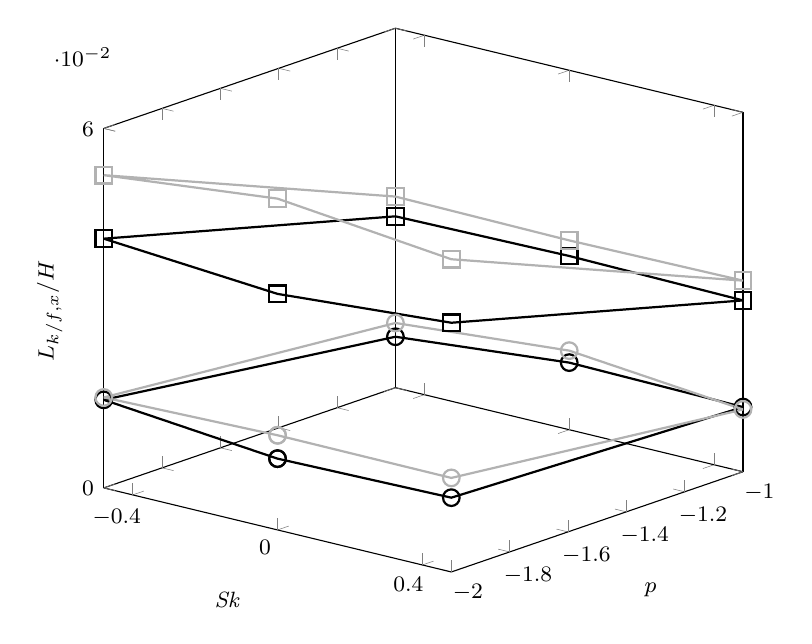
\begin{tikzpicture}[]
        \centering
        \begin{axis}[
        view={40}{20},
            ylabel={$p$},
            xlabel={\textit{Sk}},
			zlabel={$L_{k/f,x}/H$},
			xtick={-0.4,0,0.4},
			ztick={0,0.06},
			zmin=0,zmax=0.06,
            %ymin=0, ymax=0.16,
            width=.8\textwidth,
            height=.7\textwidth,
            label style={font=\footnotesize},
            tick label style={font=\footnotesize}
            ]
            
            
            
                                    \addplot3 [
            black,mark=o,thick, mark size=3pt
            ]
            coordinates{
            (0,-2,0.0119)			
			(0.48,-2,0.0124)
			(0.48,-1,0.0108)
			(0,-1,0.0112)
			(-0.48,-1,0.0085)
			(-0.48,-2,0.0147)
            (0,-2,0.0119)
			};
			\addplot3 [
            gray!60,mark=o,thick, mark size=3pt
            ]
            coordinates{
            (0,-2,0.0158)
			(0.48,-2,0.0157)
			(0.48,-1,0.0104)
			(0,-1,0.0132)
			(-0.48,-1,0.0108)
			(-0.48,-2,0.0151)
			(0,-2,0.0158)
            };
            
            
        
            
                                    \addplot3 [
            black,mark=square,thick, mark size=3pt
            ]
            coordinates{
            (0,-2,0.0394)			
			(0.48,-2,0.0416)
			(0.48,-1,0.0286)
			(0,-1,0.0290)
			(-0.48,-1,0.0286)
			(-0.48,-2,0.0416)
            (0,-2,0.0394)
			};
			\addplot3 [
            gray!60,mark=square,thick, mark size=3pt
            ]
            coordinates{
            
            (0,-2,0.0553)
			(0.48,-2,0.0522)
			(0.48,-1,0.0319)
			(0,-1,0.0316)
			(-0.48,-1,0.0319)
			(-0.48,-2,0.0522)
			(0,-2,0.0553)
            };
            
        \end{axis}
        \end{tikzpicture}
    %\caption{Streamwise.}
    %\end{subfigure}\hfill
    %    \begin{subfigure}{0.48\linewidth}
    %    \centering
    %        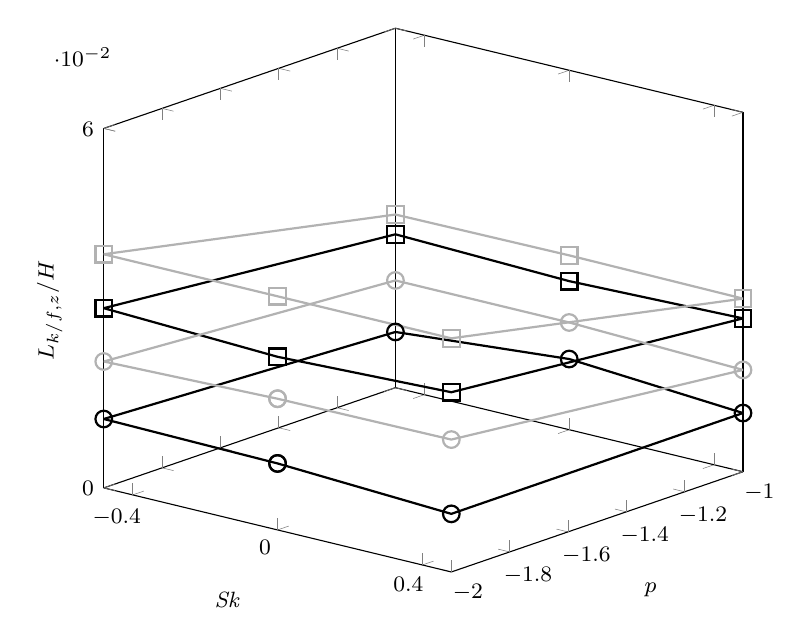
\begin{tikzpicture}[]
        \centering
        \begin{axis}[
        view={40}{20},
            ylabel={$p$},
            xlabel={\textit{Sk}},
			zlabel={$L_{k/f,z}/H$},
			xtick={-0.4,0,0.4},
			ztick={0,0.06},
			zmin=0,zmax=0.06,
            %ymin=0, ymax=0.16,
            width=.8\textwidth,
            height=.7\textwidth,
            label style={font=\footnotesize},
            tick label style={font=\footnotesize}
            ]

            
                                    \addplot3 [
            black,mark=square,thick, mark size=3pt
            ]
            coordinates{
            (0,-2,0.0289)			
			(0.48,-2,0.0300)
			(0.48,-1,0.0256)
			(0,-1,0.0248)
			(-0.48,-1,0.0256)
			(-0.48,-2,0.0300)
            (0,-2,0.0289)
			};
			
			
			\addplot3 [
            gray!60,mark=square,thick, mark size=3pt
            ]
            coordinates{
            
            (0,-2,0.0390)
			(0.48,-2,0.0390)
			(0.48,-1,0.0289)
			(0,-1,0.0291)
			(-0.48,-1,0.0289)
			(-0.48,-2,0.0390)
			(0,-2,0.0390)
            };
            
            
                                                            \addplot3 [
            black,mark=o,thick, mark size=3pt
            ]
            coordinates{
            (0,-2,0.0111)		
			(0.48,-2,0.0097)
			(0.48,-1,0.0098)
			(0,-1,0.0118)
			(-0.48,-1,0.0093)
			(-0.48,-2,0.0115)
            (0,-2,0.0111)
			};
			\addplot3 [
            gray!60,mark=o,thick, mark size=3pt
            ]
            coordinates{
            (0,-2,0.0219)
			(0.48,-2,0.0221)
			(0.48,-1,0.0170)
			(0,-1,0.0179)
			(-0.48,-1,0.0179)
			(-0.48,-2,0.0211)
			(0,-2,0.0219)
            };
            
            
        \end{axis}
        \end{tikzpicture}
    %\caption{Spanwise.}
    %\end{subfigure}
    %\caption{Integral length scale $L_k$ and $L_f$ as functions of $Sk$ and $p$. The squares represent $L_k$ while circles represent the $L_f$. Black: $\lambda_0=0.8H$, gray: $\lambda_0=1.6H$.}
%    \label{IntLength}
%\end{figure}






%\begin{figure}
%    \centering
%    \begin{subfigure}{0.48\linewidth}
%    \centering
%            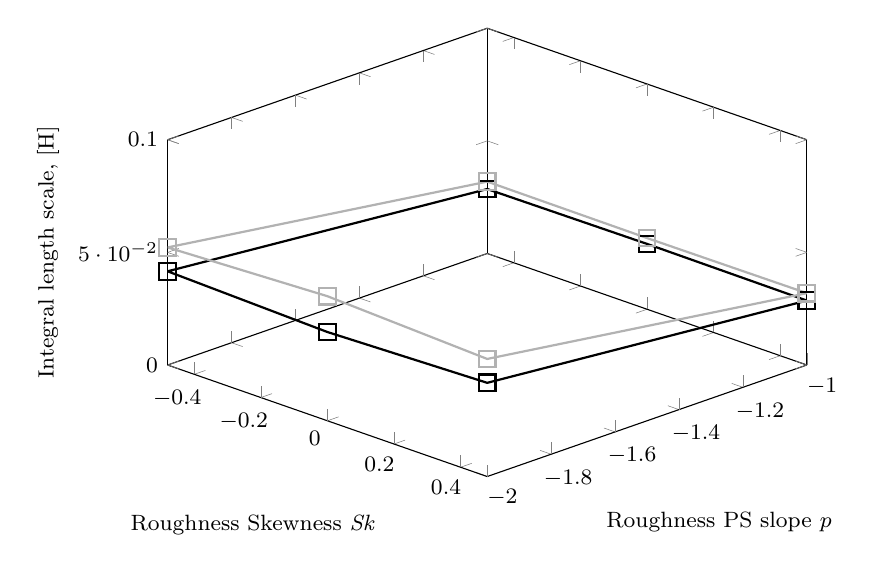
\begin{tikzpicture}[]
        \centering
        \begin{axis}[
        view={45}{35},
            ylabel={Roughness PS slope $p$},
            xlabel={Roughness Skewness \textit{Sk}},
			zlabel={Integral length scale, [H]},
			%ztick={0, 0.02,0.04,0.06,0.08},
			zmin=0,zmax=0.1,
            %ymin=0, ymax=0.16,
            width=.8\textwidth,
            height=.6\textwidth,
            label style={font=\footnotesize},
            tick label style={font=\footnotesize}
            ]
            
            
                                    \addplot3 [
            black,mark=square,thick, mark size=3pt
            ]
            coordinates{
            (0,-2,0.0394)			
			(0.48,-2,0.0416)
			(0.48,-1,0.0286)
			(0,-1,0.0290)
			(-0.48,-1,0.0286)
			(-0.48,-2,0.0416)
            (0,-2,0.0394)
			};
			\addplot3 [
            gray!60,mark=square,thick, mark size=3pt
            ]
            coordinates{
            
            (0,-2,0.0553)
			(0.48,-2,0.0522)
			(0.48,-1,0.0319)
			(0,-1,0.0316)
			(-0.48,-1,0.0319)
			(-0.48,-2,0.0522)
			(0,-2,0.0553)
            };
            
        \end{axis}
        \end{tikzpicture}
%    \end{subfigure}
%        \begin{subfigure}{0.48\linewidth}
%        \centering
%            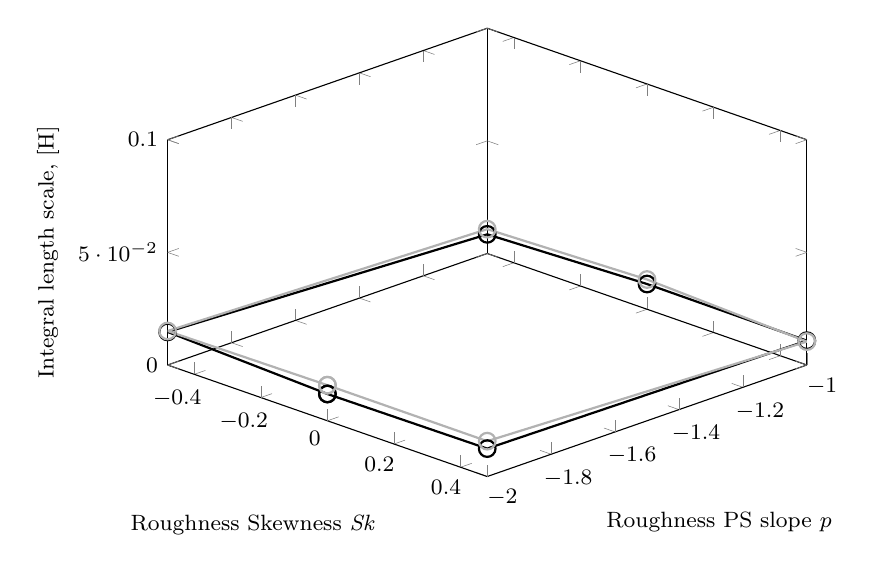
\begin{tikzpicture}[]
        \centering
        \begin{axis}[
        view={45}{35},
            ylabel={Roughness PS slope $p$},
            xlabel={Roughness Skewness \textit{Sk}},
			zlabel={Integral length scale, [H]},
			%ztick={0, 0.02,0.04,0.06,0.08},
			zmin=0,zmax=0.1,
            %ymin=0, ymax=0.16,
            width=.8\textwidth,
            height=.6\textwidth,
            label style={font=\footnotesize},
            tick label style={font=\footnotesize}
            ]
            
            
            
                                    \addplot3 [
            black,mark=o,thick, mark size=3pt
            ]
            coordinates{
            (0,-2,0.0119)			
			(0.48,-2,0.0124)
			(0.48,-1,0.0108)
			(0,-1,0.0112)
			(-0.48,-1,0.0085)
			(-0.48,-2,0.0147)
            (0,-2,0.0119)
			};
			\addplot3 [
            gray!60,mark=o,thick, mark size=3pt
            ]
            coordinates{
            (0,-2,0.0158)
			(0.48,-2,0.0157)
			(0.48,-1,0.0104)
			(0,-1,0.0132)
			(-0.48,-1,0.0108)
			(-0.48,-2,0.0151)
			(0,-2,0.0158)
            };
            
        \end{axis}
        \end{tikzpicture}
%    \end{subfigure}
%    \caption{Integral length scale of $k$ (left) and $f_x$ (right) as functions of roughness skewness and roughness PS slope. Color indicates roughness upper cutoff wavelength, Black: $\lambda_0=0.8H$, gray: $\lambda_0=1.6H$.}
%    \label{IntLength}
%\end{figure}
\subsubsection{Coherence function of surface force and roughness}
\label{coherence}
\begin{figure}
    \centering
   \begin{subfigure}[b]{0.49\linewidth}
   \centering
            \begin{tikzpicture}[]
        \centering
        \begin{axis}[
            ylabel={$\overline{\gamma_{kf}^2}$},
            xlabel={$\lambda/H$},
            ymin=0, ymax=.8,
			xmin=0.01,xmax=2.4,
            width=1\textwidth,
            height=.9\textwidth,
			xmode=log,
			  axis y line*=left,
      axis x line*=bottom,
            legend style={font=\tiny,anchor=north west},
                        legend pos=north west,
            label style={font=\footnotesize},
            tick label style={font=\footnotesize}
            ]
            % \fill[color=black!30,opacity=50] (0.8,0) -- (0.8,1) -- (2,1) -- (2,0) -- cycle;
            %  \fill[color=black!60,opacity=90] (1.6,0) -- (1.6,1) -- (2,1) -- (2,0) -- cycle;
     \node[label={[rotate=-90]{\color{red}\tiny$\Delta_x=0.3-0.6H$}}] at (axis cs:0.6,0.2) {};
	 \fill[color=red!20,opacity=20] (0.3,0.9) -- (0.6,0.9) -- (0.6,-0.1) -- (0.3,-0.1) -- cycle;
	                                     			            \addplot [
            black,dashdotted,thick,
            ]
            table [x=X, y=Y,col sep=comma]{CSV/Coh_G4.csv};
            \addlegendentry{$G14M2-500$}
			            \addplot [
            black,solid,thick,
            ]
            table [x=X, y=Y,col sep=comma]{CSV/Coh_G3.csv};
            \addlegendentry{$G24M2-500$}
	             			            \addplot [
            black,dashed,thick,
            ]
            table [x=X, y=Y,col sep=comma]{CSV/Coh_G2.csv};
            \addlegendentry{$G18M1-500$}
                                    \addplot [
            black,dotted,thick,
            ]
            table [x=X, y=Y,col sep=comma]{CSV/Coh_G1.csv};
            \addlegendentry{$G28M1-500$}

			
			
\draw [dashed,red] (0.08,0) -- (0.08,1);
\draw[->] (0.7,0.6) -- (1.5,0.6);
\node[] at (1.03,0.65) {{\tiny Wavy scales}};

			            \addplot[
            red,mark=o, only marks, mark size=1pt
            ]
            coordinates{
            (0.4062,0.562)%G24
			};                         \addplot[
            red,mark=o, only marks, mark size=1pt
            ]
            coordinates{
            (0.3047,0.52)%G14
            (0.3563,0.54)%18
            (0.6,0.557)%28
			};
        \end{axis}
            \begin{axis}[
            xlabel={$\lambda^+$},
                        ymin=0, ymax=.8,
                                    width=1\textwidth,
            height=.9\textwidth,
			xmin=5,xmax=1200,
			axis y line*=right,
			domain=5:1200,
			xmode=log,
yticklabels={,,},
      axis x line*=top]
    \end{axis}
    
        \end{tikzpicture}    
    \caption{streamwise}
    \end{subfigure}\hfill
        \begin{subfigure}[b]{0.49\linewidth}
    \centering
            \begin{tikzpicture}[]
        \centering
        \begin{axis}[
            ylabel={$\overline{\gamma_{kf}^2}$},
            xlabel={$\lambda/H$},
            ymin=0, ymax=.8,
			xmin=0.01,xmax=2.4,
            width=1\textwidth,
            height=.9\textwidth,
			xmode=log,
            legend style={font=\tiny,anchor=south east},
                        legend pos=south east,
            label style={font=\footnotesize},
            tick label style={font=\footnotesize}
            ]
            % \fill[color=black!30,opacity=50] (0.8,0) -- (0.8,1) -- (2,1) -- (2,0) -- cycle;
            %  \fill[color=black!60,opacity=90] (1.6,0) -- (1.6,1) -- (2,1) -- (2,0) -- cycle;
                \addplot [
            black,dashdotted,thick,
            ]
            table [x=X, y=Y,col sep=comma]{CSV/Coh_GSpan4.csv};
            \addlegendentry{$G14M2-500$}
			            \addplot [
            black,dotted,thick,
            ]
            table [x=X, y=Y,col sep=comma]{CSV/Coh_GSpan3.csv};
            \addlegendentry{$G24M2-500$}
            			            \addplot [
            black,dashed,thick,
            ]
            table [x=X, y=Y,col sep=comma]{CSV/Coh_GSpan2.csv};
            \addlegendentry{$G18M1-500$}
                        \addplot [
            black,solid,thick,
            ]
            table [x=X, y=Y,col sep=comma]{CSV/Coh_GSpan1.csv};
            \addlegendentry{$G28M1-500$}

          %              			            \addplot [
           % red,solid,thick,
        %    ]
        %    table [x=X, y=Y,col sep=comma]{CSV/Coh_G24M1Span1.csv};
         %   \addlegendentry{G24M1}
		%	            \addplot [
         %   black!60,solid,thick,
          %  ]
           % table [x=X, y=Y,col sep=comma]{CSV/Coh_PSpan2.csv};
        %    			            \addplot [
        %    black!60,dashed,thick,
        %    ]
        %    table [x=X, y=Y,col sep=comma]{CSV/Coh_GSpan2.csv};
	%		            \addplot [
    %        black!60,dotted,thick,
    %%        ]
     %       table [x=X, y=Y,col sep=comma]{CSV/Coh_NSpan2.csv};
%						            \addplot [
 %           black!30,solid,thick,
  %          ]
   %         table [x=X, y=Y,col sep=comma]{CSV/Coh_PSpan3.csv};
    %        			            \addplot [
     %       black!30,dashed,thick,
      %%     table [x=X, y=Y,col sep=comma]{CSV/Coh_GSpan3.csv};
		%	            \addplot [
         %   black!30,dotted,thick,
          %  ]
          %  table [x=X, y=Y,col sep=comma]{CSV/Coh_NSpan3.csv};
	%					            \addplot [
    %        black!10,solid,thick,
    %        ]
    %        table [x=X, y=Y,col sep=comma]{CSV/Coh_PSpan4.csv};
    %        			            \addplot [
    %        black!10,dashed,thick,
    %        ]
    %       table [x=X, y=Y,col sep=comma]{CSV/Coh_GSpan4.csv};
%			            \addplot [
%            black!10,dotted,thick,
%            ]
 %           table [x=X, y=Y,col sep=comma]{CSV/Coh_NSpan4.csv};			
			
			
\draw [dashed,red] (0.08,0) -- (0.08,1);

        \end{axis}
                    \begin{axis}[
            xlabel={$\lambda^+$},
                        ymin=0, ymax=.8,
                                    width=1\textwidth,
            height=.9\textwidth,
			xmin=5,xmax=1200,
			axis y line*=right,
			domain=5:1200,
			xmode=log,
yticklabels={,,},
      axis x line*=top]
    \end{axis}
        \end{tikzpicture}    
    \caption{spanwise}
    \end{subfigure}
\caption{Mean coherence function $\bar{\gamma}_{kf}^2$ as a function of $\lambda=2\pi/q$ normalized by $H$, $\lambda_1=0.08H$ is marked by vertical dashed lines on the left and right side, respectively. $\lambda^+$ for the current cases $Re_\tau\approx500$ is shown on the upper axis. The length scale of force separation obtained from its auto-correlation functions are marked by red circles on each coherence function respectively.} %In (b), $\lambda=0.08H$ and $\lambda=0.6H$ are represented by vertical dashed lines on the left and right side, respectively.}
    \label{Coh_Lambda}
\end{figure}
To further understand the correlation between force and height distributions at different roughness length scales, coherence function between the two distributions is calculated. % and discussed in the following.
%More insight into the correlation of forcing reaction with roughness structure in terms of different roughness scale is obtained by analysing coherence functions.
The coherence function represents the correlation of force distribution with roughness height distribution as a function of wavenumber:
\begin{equation}
    \gamma_{kf}^2(q)=\frac{|E_{kf}(q)|^2}{E_{f}(q)E_{k}(q)},
\end{equation}
where $E_{kf}(q)$ represents cross-PS of roughness topography $k(x,z)$ and force map $f_x(x,z)$, while $E_{f}(q)$ represents the PS of $f_x(x,z)$.
Power spectra are calculated based on 1D distribution profiles along streamwise and spanwise directions, and the mean coherence function $\overline{\gamma_{kf}^2}$ is obtained by averaging each parallel signal pairs.
Figure~\ref{Coh_Lambda} shows the mean coherence function of Gaussian surfaces in (a) streamwise direction and (b) spanwise direction as a function of wavelength $\lambda={2\pi}/{q}$ -- upper axis shows inner scaled wavelength $\lambda^+$ at $Re_\tau=500$.
It is worth reminding that for all topographies, the smallest in-plane roughness scale is prescribed to be $\lambda_1=0.08H$.
This is clearly related to the observation that coherence functions are significantly smaller below $\lambda\approx0.08H$ ($\lambda^+\approx40$).
Above this threshold, coherence functions increase and retain high values until a certain wavelength, which is roughly at $\lambda\approx0.3-0.6H$ ($\lambda^+\approx150-300$) for the studied cases.
With further evolution of the coherence function to larger wavelengths, the coherence decreases monotonically.
Similar observations are made for negatively and positively skewed roughness. %, that the surface structure with wavelength ranging between $\lambda_1=0.08H$ and $\lambda\approx0.3-0.6H$ shows significant coherence with the surface force.
%It can be said that t
The force becomes less correlated with the surface features at very large scale, or in other words, very large wavelengths in streamwise direction do not contribute to the generation of surface force.
These length scales might be related to the `wavy roughness' concept stemming from the observations by~\citet{Schultz2009}. \cite{BARROS20181} stated that these length scales can be filtered out in regard of determining the skin friction.%skin friction as much as they do to the mean square surface height.

Notably, the streamwise wavelength at which the coherence starts to drop has a similar value to the streamwise separation distance of the surface force peaks.
A comparison between the coherence dropping wavelength $\lambda_{\text{Coh}}$ and the length scale of force peak separation $\lambda_{f}$ is conducted in figure~\ref{corrcohlength}.
It can be observed that all data points are clustering around $\lambda_{\text{Coh}}=\lambda_{f}$ (dotted line) indicating a clear correspondence of these length scales.
%As discussed before, the latter quantity is related to the sheltering effect, which suggests that the sheltering distance can be a possible characteristic scale for estimating the extent by which drag force remains correlated to the surface height.
The significant coherence at relative small length scales might be linked to the interaction of roughness structure and sheltering.
As discussed before, the occurrence of extreme force peaks is strongly determined by the roughness areas that are exposed in the high-momentum flow, or outside the sheltering.
Thus, streamwise recurring force peaks caused by sheltering can be found in figure~\ref{G24Force_Dist}.
Small magnitude of force peaks can be found between two successive extreme peaks, which contributes to the coherence function at small wavelength.
Furthermore, the roughness structures whose length scales are comparable to the distance between two successive extreme peaks, i.e. $\lambda_f$, show significance in the coherence function at corresponding wavelength.
Beyond this length scale, no larger force peak separation can be found, the coherence function keeps decreasing into large wavelength region.
%The separation of these force peaks can be arbitrarily small as long as the surface is stretching out of the sheltering area, thus the high coherence in relative small wavelength range is observed.
%On the other hand, the largest separation distance of extreme force peaks is bounded because the high-momentum flow gradually reattaches the ground in a certain distance, the next extreme force peak is formed within this distance.
%As a consequence, the coherence functions show significant values within a certain range of small wavelengths and keep decreasing beyond a large wavelength 
%Due to the weakened correlation with surface force these large scales of roughness are labeled as 'wavy scales' stemming from the observation by~\citet{Schultz2009} which can be filtered out in regard of determining the skin friction~\citep{BARROS20181}. It must be noted that \citet{Schultz2009} suggest a distinction between `wavy' or `rough' scales based on their effective slope based. 

%The correlation of roughness elements and surface force is thus limited within the sheltered area bounded by extreme force peaks, i.e. the high coherence wavelengths are bounded by the separation of extreme force peaks.
%From figure~\ref{Coh_Lambda} the dropping point of the coherence function at $\lambda\approx0.5H$ is detected.
%This value agrees with the estimation in previous section that the surface peak separations have values approximately equal $0.5H$ as the consequence of the sheltering cycle.}\\
%This dominant wavelength region can be an indication that a certain range of streamwise roughness wavelengths contribute the most to the generation of drag.
Figure \ref{Coh_Lambda}(b) demonstrates that, unlike the tortuous behavior exhibited by the streamwise mean coherence function, the spanwise mean coherence function shows a monotonically increasing trend before a plateau at larger wavelengths. %The cases studied in this work do not show any drop in the coherence function at large spanwise wavelengths. It should be reminded that the coherence functions have different extents on the wavelength axis as a result of limited spanwise size of minimal channels $M$2 and $M$1. \\

%\begin{figure}
%    \centering
%    \begin{subfigure}{0.49\l%inewidth}
%   \centering
%            \begin{tikzpicture}[]
        \centering
        \begin{axis}[
            ylabel={$\overline{\gamma_{kf}^2}$},
            xlabel={$\lambda/H$},
            ymin=0, ymax=.8,
			xmin=0.01,xmax=2.4,
            width=1\textwidth,
            height=.9\textwidth,
			xmode=log,
            legend style={font=\tiny,anchor=south east},
                        legend pos=south east,
            label style={font=\footnotesize},
            tick label style={font=\footnotesize}
            ]
            % \fill[color=black!30,opacity=50] (0.8,0) -- (0.8,1) -- (2,1) -- (2,0) -- cycle;
            %  \fill[color=black!60,opacity=90] (1.6,0) -- (1.6,1) -- (2,1) -- (2,0) -- cycle;
            \addplot [
            black,solid,thick,
            ]
            table [x=X, y=Y,col sep=comma]{CSV/Coh_Re1.csv};
            \addlegendentry{$G24M2-1000$}
            			            \addplot [
            black,dashed,thick,
            ]
            table [x=X, y=Y,col sep=comma]{CSV/Coh_Re2.csv};
            \addlegendentry{$G24M2-750$}
			            \addplot [
            black,dotted,thick,
            ]
            table [x=X, y=Y,col sep=comma]{CSV/Coh_Re3.csv};
            \addlegendentry{$G24M2-500$}
            			            \addplot [
            black,dashdotted,thick,
            ]
            table [x=X, y=Y,col sep=comma]{CSV/Coh_Re4.csv};
            \addlegendentry{$G24M2-250$}
%\draw [dashed,red] (0.08,0) -- (0.08,1);
%\draw [dashed,red] (0.6,0) -- (0.6,1);
\draw [dashed,red] (0.08,0) -- (0.08,1);
\draw[->] (0.6,0.7) -- (0.15,0.7);
\node[] at (0.3,0.74) {$Re_\tau$};


        \end{axis}
        \end{tikzpicture}    
%    \caption{Outer scaling}
%    \end{subfigure}\hfill
%    \begin{subfigure}{0.49\linewidth}
%    \centering
%            \begin{tikzpicture}[]
        \centering
        \begin{axis}[
            ylabel={$\overline{\gamma_{kf}^2}$},
            xlabel={$\lambda^+$},
            ymin=0, ymax=.8,
			xmin=0.01*500,xmax=2.4*500,
            width=1\textwidth,
            height=.9\textwidth,
			xmode=log,
            legend style={font=\tiny,anchor=south east},
                        legend pos=south east,
            label style={font=\footnotesize},
            tick label style={font=\footnotesize}
            ]
            % \fill[color=black!30,opacity=50] (0.8,0) -- (0.8,1) -- (2,1) -- (2,0) -- cycle;
            %  \fill[color=black!60,opacity=90] (1.6,0) -- (1.6,1) -- (2,1) -- (2,0) -- cycle;
            \addplot [
            black,solid,thick,
            ]
            table [x=X, y=Y,col sep=comma]{CSV/Coh_RePlus1.csv};
 \addlegendentry{$G24M2-1000$}
            			            \addplot [
            black,dashed,thick,
            ]
            table [x=X, y=Y,col sep=comma]{CSV/Coh_RePlus2.csv};
 \addlegendentry{$G24M2-750$}
			            \addplot [
            black,dotted,thick,
            ]
            table [x=X, y=Y,col sep=comma]{CSV/Coh_RePlus3.csv};
 \addlegendentry{$G24M2-500$}
 			            \addplot [
            black,dashdotted,thick,
            ]
            table [x=X, y=Y,col sep=comma]{CSV/Coh_RePlus4.csv};
 \addlegendentry{$G24M2-250$}
 %\draw [dashed,red] (0.08*500,0) -- (0.08*500,1);
\draw [dashed,red] (0.6*500,0) -- (0.6*500,1);
\draw [dashed,red] (0.08*500,0) -- (0.08*500,1);
\draw[->] (15,0.3) -- (90,0.3);
\node[] at (26,0.34) {$Re_\tau$};

        \end{axis}
        \end{tikzpicture}    
%    \vspace{-0.5cm}
%    \caption{Inner scaling}
%    \end{subfigure}
%\caption{Streamwise mean coherence function $\bar{\gamma}^2_{kf}$ as function of wavelength $\lambda=2\pi/q$. dashed lines indicating $\lambda_1=0.08H$ and $\lambda=0.6H$ in (a) and correspondingly $\lambda_1^+=40$ and $\lambda^+=300$ in (b) are kept from previous figure. The magnitude of cross-correlation coefficient increases with $k^+$, i.e. from -0.42 to -0.59.}
%    \label{Coh_Re}
%\end{figure}
%In order to investigate the behaviour of coherence function in the range of considered $Re_\tau$, streamwise coherence function of the topography $G24M2$ with $Re_\tau\approx250$, $500$, $750$ and $1000$ are compared in figure~\ref{Coh_Re}.
%{\color{red}The red dashed line indicates the smallest roughness wavelength $\lambda_1=0.08H$.
%Gradual shift of the coherence function peak is observed with increasing $Re_\tau$.
%The coherence function of the case $G24M2$-250 monotonically decreases at relative larger wavelength comparing to other cases.
%This can be understood by comparing the velocity profiles in figure~\ref{Re_expand}, the inner-scaled velocities at roughness tips $k_t$ show decreasing trend with increasing $Re_\tau$.
%From the wake expansion rate $\tan\theta=C_\theta u_\tau/U_h$, higher inner-scaled velocity corresponds to milder wake expansion, which leads to a larger separation of extreme surface force peaks.
%Consequently, the coherence of roughness and surface force is extended to larger wavelength.
%Furthermore, the reduced sheltering length results in the increase of cross correlation coefficient from -0.42 to -0.59 due to the fact that less roughness structures are sheltered}
%{\color{gray}Red dashed lines indicating the influential wavelength range are kept identical to those in figure~\ref{Coh_Lambda} for comparison.
%From comparison of figures~\ref{Coh_Re}(a \& b) it is observed that the peaks of coherence functions align better when plotted against inner scaled wavelength. One can observe in figure~\ref{Coh_Re}(b) that coherence functions in all cases start decreasing at $\lambda^+\approx300$. Among all cases, that at $Re_\tau=250$ shows some early decrease in coherence function, which can be attributed to the limited largest in-plane wavelength in wall unit $\lambda_0^+=200<300$. The left sides of coherence function curves collapse when plotted in outer units since the smallest wavelength in the simulations is a fixed factor in $H$. }\\

%Overall the results presented in this section can be regarded as a hint that, at a certain range of roughness wavelengths, namely $\lambda\lessapprox0.5H$, surface force responds more directly to the spatial fluctuation of rough surface.



%On the left panel, the mean coherence function is plotted as a function of $\lambda$ in channel half height units, $H$ (outer scaling). Here a systematic shift of the coherence peaks to lower wavelengths can be observed with increasing $Re_\tau$.
%Notably, for the case $G24M2-250$, the peak extends to wavelength $\lambda>0.6H$.
%Thus, on the right panel, coherence functions are plotted against inner-scaled $\lambda^+$.
%Good alignment of the coherence peak position in terms of $\lambda^+$ is obtained.
%Furthermore, albeit $\lambda^+$ remains different at different $Re_\tau$, coherence function show similar trend. 
%The shift of the peak shoulders on the small wavelength side is due to the fact that the smallest in-plane wavelength in wall unit, $\lambda_1^+$, increases with $Re_\tau$ as shown in figure~\ref{Coh_Re}(b).
%The coherence functions simultaneously decreases from the previously detected wavelength in wall unit, i.e. $\lambda^+\approx300$, as marked by the red dashed line.
%For a comparison, the inner scaled upper cutoff wavelength $\lambda_0^+=$200, 400, 600 and 800 for $Re_\tau=250$, 500, 750 and 1000 respectively. 
%From these observations, the upper dominant wavelength region border in wall unit, i.e. $\lambda^+\lessapprox300$, applies for all investigated cases.
%The early decrease of coherence function at $Re_\tau=250$ is likely due to the limited largest in-plane wavelength in wall unit $\lambda_0^+=200<300$.
%In conclusion, it is found that within a certain range of roughness wavelength, namely $\lambda^+\lessapprox300$, streamwise forcing statistics respond to the spatial fluctuation of rough surface significantly.
%However, for present topographies the smallest in-plane scale $\lambda_1=0.08H$ is limited, thus the lower bound of the dominant wavelength region has potential to extend when smaller roughness scales are simulated.
%This can also be seen from coherence function of $G24M2-250$ in figure~\ref{Coh_Re}(b).
%Due to the lower $Re_\tau$, roughness structures are smaller in wall unit, among those smaller structures, peaks can be observed at $\lambda^+<40$ (corresponds to $\lambda_1=0.08H$ at $Re_\tau=500$).
%In contrary, the upper bound of the wavelength region is covered by the largest in-plane roughness scale $\lambda_0^+$ in most of the cases.

%Therefore, it is safe to conclude that the force is significantly correlated with the roughness length scale $\lambda^+\lessapprox300$.
%Beyond this threshold, the impact of roughness structures on the force starts to decrease.
%The roughness scales within this length scale range can be most dominant to its hydrodynamic property, e.g. skin friction.

%The physical interpretation of the length scale $\lambda^+\approx300$ can be related to the near wall turbulent cycle in buffer layer as reported in previous studies~\citep{jimenez_moin_1991,jeong_hussain_schoppa_kim_1997}.
%The near wall quasi-streamwise turbulent structures measure $200-300$ viscous units, with comparable length scale of the wall structures the interaction of flow and surface are of crucial dominance, i.e. the near wall flow structures can be effectively interfered by the small roughness structures with $\lambda^+\leq300$ while those roughness structures with larger length scales $\lambda^+\geq300$ are regarded as curved surfaces rather than roughness, from the standpoint of the flow.

\begin{figure}
    \centering
            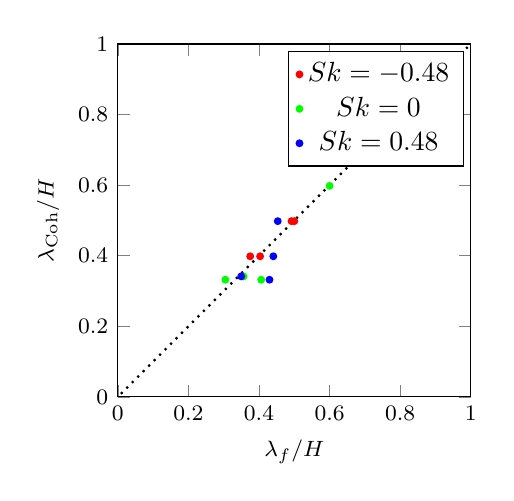
\begin{tikzpicture}[]
        \centering
        \begin{axis}[
            ylabel={$\lambda_{\text{Coh}}/H$},
			xlabel={$\lambda_f/H$},
			%xtick={-2,-1},
			%ytick={0,0.04,0.08},
			ymin=0,ymax=1,
			xmin=0,xmax=1,
            %ymin=0, ymax=0.16,
            width=.5\textwidth,
            height=.5\textwidth,
            label style={font=\footnotesize},
            tick label style={font=\footnotesize}
            ]
 \addplot [
           red,mark=*,only marks,thick, mark size=1pt
           ]
           coordinates{
		(0.4922,0.498)
            (0.5,0.498)
            (0.3750,0.3984)
            (0.4031,0.3984)
			};
			            \addlegendentry{$Sk=-0.48$}
\addplot [
            green,mark=*,only marks,thick, mark size=1pt
            ]
            coordinates{
            (0.3047,0.332)
            (0.4062,0.332)
            (0.3563,0.3415)
            (0.6,0.598)};
\addlegendentry{$Sk=0$}
               \addplot [
           blue,mark=*,only marks,thick, mark size=1pt
            ]
            coordinates{
            (0.4297,0.332)%P
           (0.4531,0.498)
            (0.3496,0.3415)
            (0.4406,0.3984)%
			};
			\addlegendentry{$Sk=0.48$}%
			\addplot [
            black,mark=square,thick,dotted,mark size=3pt
            ]
           coordinates{%
			(-0.1,-0.1)
			(1.1,1.1)
           };
        \end{axis}
        \end{tikzpicture}
    \caption{The length scale of force peak separation detected from the auto-correlation functions $\lambda_{f}$ compared with the coherence dropping wavelength $\lambda_{\text{Coh}}$.}
    \label{corrcohlength}
\end{figure}



\subsection{Effect of topographical properties}
\label{results}
 In~\cref{Rando}, we discussed the applicability of minimal channel concept for characterization of realistic roughness. In doing so, we examined a relatively large number of roughness topographies. This provides a basis for studying the effect of roughness topography on hydrodynamic properties of the surface, here $\Delta U^+$ and $d^+$. The present section is devoted to this task.
 As discussed in previous sections, minimal channels are capable for indicating the hydrodynamic behaviour of roughness.
 Thus, the bold values in table~\ref{ResultAll}, which are regarded as the minimal channel results, will be used in this section.
 
 \subsubsection{Roughness function}
 An overview of the roughness function $\Delta U^+$ from minimal channel simulations is plotted in figure~\ref{fig-3d}, where roughness function $\Delta U^+$ is shown as a function of two of the investigated roughness parameters, i.e. skewness $Sk$ and PS slope $p$.
 %Where color indicates different $\lambda_0$, black: $\lambda_0=0.8H$, gray: $\lambda_0=1.6H$.
%It is noted in the previous section that three types of skewness are examined here, positive skewness $Sk=0.48$, zero skewness $Sk=0$ and negative skewness  $Sk=-0.48$. 
The PDFs of the considered topographies are shown in figure~\ref{fig:HPDS}(a).
In figure~\ref{fig-3d} the corresponding effect of $Sk$ on the retardation of mean velocity profile is shown.
%\begin{figure}[ht]
%    \centering
%    \begin{subfigure}[t]{.5\linewidth}
%             \begin{tikzpicture}[]
        \centering
        \begin{axis}[
            ylabel={PDF},
            xlabel={k/H},
            ymax=0.05,
            width=.8\textwidth,
            height=.8\textwidth,
            legend style={font=\tiny,anchor=north west,fill=none},
            legend pos=north west,
            legend cell align={left},
            label style={font=\footnotesize},
            tick label style={font=\footnotesize}
            ]
            \addplot [
            black,solid,thick,
            ]
            table [x=X, y=Y,col sep=comma]{CSV/HPDG14F1.csv};
    \node[black,right] at (axis cs: -0.01,0.025) {$Sk=0.48$};
			\addplot [
            black,dashed,thick,
            ]
            table [x=X, y=Y,col sep=comma]{CSV/HPDN14F1.csv};
    \node[black] at (axis cs: 0.061,0.03) {$Sk=0$};
						\addplot [
            black,dotted,thick,
            ]
            table [x=X, y=Y,col sep=comma]{CSV/HPDP14F1.csv};
    \node[black,right] at (axis cs: 0.07,0.025) {$Sk=-0.48$};
        \end{axis}
        \end{tikzpicture}

%    \caption{PDF of roughness. \full: $Sk=0$, \dashed: $Sk=-0.48$, \dotted: $Sk=0.48$}
%    \end{subfigure}\hfill%
%    \begin{subfigure}[t]{.5\linewidth}
%    \begin{tikzpicture}
\begin{loglogaxis}[
		xlabel={$q/q_{\text{ref}}$},
		ylabel={$q_{\text{ref}}E_k(q)/k_{\text{rms}}^2$},
		xmin=0.1,xmax=100,
		ymin=0.000001,ymax=10,
		%ticks=none,
		clip=true,
		set layers,
		clip mode=individual,
		height=.8\textwidth,
		width=.8\textwidth,
        label style={font=\footnotesize},
        tick label style={font=\footnotesize}
		%axis line style={draw opacity=0}
		%xtick={0,800,...,2400},
		%colorbar,
		%point meta min=0,
		%point meta max=1.11,
		%colorbar style={
		%ytick={0,0.2,...,1.11}
		%}
	]
	\centering
\addplot [thick, color=blue, on layer=axis background]
graphics[xmin=0.1,ymin=0.000001,xmax=100,ymax=10]{Figures/PS_p.png};
    \draw[red,dashed,thick] (1,0.000001) -- (1,10);
    \draw[red,dashed,thick] (10,0.000001) -- (10,10);
    \node[label={[rotate=-90]{\scriptsize$\lambda=0.8H$}}] at (axis cs:1.05,0.5) {};
                \node[label={[rotate=-90]{\scriptsize$\lambda=0.08H$}}] at (axis cs:10.05,0.5) {};
    \draw[red] (1.3,0.08161) -- (1.803,0.08161);
    \draw[red] (1.803,0.05) -- (1.803,0.08161);                
        \node[black,right] at (axis cs: 1.803,0.07) {{\tiny $p=-2$}};
        
        \draw[red] (5.3,0.009) -- (9,.009);
    \draw[red] (9,0.009) -- (9,0.0056);                
        \node[black,right] at (axis cs: 9,0.007) {{\tiny $p=-1$}};
\end{loglogaxis}
\end{tikzpicture}
%    \caption{PS with different $p$ with $\lambda_0=0.4H$, wavenumber $q$ is normalized by %referencing wavenumber $q_0=\frac{2\pi}{\lambda_0}$.}
%    \end{subfigure}
%    \begin{subfigure}[t]{.5\linewidth}
%    \begin{tikzpicture}
\begin{loglogaxis}[
		xlabel={$q/q_{\text{ref}}$},
		ylabel={$q_{\text{ref}}E_k(q)/k_{\text{rms}}^2$},
		xmin=0.1,xmax=100,
		ymin=0.000001,ymax=10,
		%ticks=none,
		clip=true,
		set layers,
		clip mode=individual,
		height=.8\linewidth,
		width=.8\linewidth,
        label style={font=\footnotesize},
        tick label style={font=\footnotesize}
		%axis line style={draw opacity=0}
		%xtick={0,800,...,2400},
		%colorbar,
		%point meta min=0,
		%point meta max=1.11,
		%colorbar style={
		%ytick={0,0.2,...,1.11}
		%}
	]
	\centering
\addplot [thick, color=blue, on layer=axis background]
graphics[xmin=0.1,ymin=0.000001,xmax=100,ymax=10]{Figures/PS_l1.png};
    \draw[red,dashed,thick] (1,0.000001) -- (1,10);
    \draw[red,dashed,thick] (0.5,0.000001) -- (0.5,10);
    \draw[red,dashed,thick] (10,0.000001) -- (10,10);
    \node[label={[rotate=-90]{\scriptsize$\lambda=0.8H$}}] at (axis cs:1.05,0.5) {};
        \node[label={[rotate=-90]{\scriptsize$\lambda=1.6H$}}] at (axis cs:0.45,0.5) {};
                \node[label={[rotate=-90]{\scriptsize$\lambda=0.08H$}}] at (axis cs:10.05,0.5) {};
        \draw[red] (1.15,0.039) -- (1.803,0.039);
    \draw[red] (1.803,0.039) -- (1.803,0.025);                
        \node[black,right] at (axis cs: 1.803,0.047) {{\tiny $p=-1$}};
\end{loglogaxis}
\end{tikzpicture}
%    \caption{PS with different $\lambda_0$ with $p=-1$, wavenumber $q$ is normalized by %referencing wavenumber $q_0=\frac{2\pi}{\lambda_0}$, where $\lambda_0=0.4H$.}
%    \end{subfigure}\hfill%
%    \begin{subfigure}[t]{.5\linewidth}
%    \input{tikz/PSforl2}
%    \caption{PS with different $\lambda_0$ with $p=-2$, wavenumber $q$ is normalized by %%referencing wavenumber $q_0=\frac{2\pi}{\lambda_0}$, where $\lambda_0=0.4H$.}
%    \end{subfigure}
%    \caption{Roughness configurations, (a) shows the PDF of the roughness. In (b,c,d) PSs of %investigated rough surfaces normalized by the r.m.s. of the power spectrum are compared, vertical dashed lines are high-pass filtering and low-pass filtering corresponding to $\lambda_0\&\lambda_1$ respectively. In (c,d) black line represents the case with $\lambda_0=0.4H$ while gray $\lambda_0=0.8H$. In (b) black line represents $p=-1$, gray $p=-2$.}
%    \label{fig:HPDS}
%\end{figure}
As investigated by ~\citet{Flack2020.}, positively skewed rough surfaces give higher skin friction than non-skewed or negatively skewed roughness.
Negatively skewed surfaces show 'slip-velocity' effect~\citep{jelly_busse_2018}, which translates into a lower mean velocity retardation.
The trend observed in the present results fully agrees with what suggested by the previous researchers.

In general, $\Delta U^+$ increases with $p$. 
As illustrated in figure~\ref{fig:HPDS}(b), at $p=-2$ larger wavelengths contribute more to the roughness and at $p=-1$ \textit{vice versa}. 
These findings agree with the study by~\citet{BARROS20181} and \cref{IBMF} highlighting, that relative small length scales of roughness have a dominant role in determining hydraulic drag.
Furthermore, it can be observed that the surfaces with $\lambda_0=1.6H$ show stronger sensitivity to the change of PS slope $p$ than those with $\lambda_0=0.8H$.
Moreover, it can be observed in figure~\ref{fig-3d} that $\Delta U^+$ generally decreases with increasing $\lambda_0$.
%Different decline slope of $\Delta U^+$  as a function of $\lambda_0$ is observed by comparing the topographies with $p=-1$ and $p=-2$. 
%The effect of $\lambda_0$ can be illustrated in the PS plot shown in figure~\ref{fig:HPDS}(c, d), in which the PS with $\lambda_0= 0.8H$ and $1.6H$ are compared in pairs grouped by matched PS slope $p$.
%With larger $\lambda_0$, a wider range of roughness length scales are presented by power law. 
%Reminding that the roughness height $k=0.1H$, the presence of large scale roughness structures causes weakening of energy in smaller wavelengths.
%This can be understood by referring to figure~\ref{fig:HPDS} (c, d), where PS density is normalized, slight downward shift of the PS can be observed for the topographies with $\lambda_0=1.6H$ comparing to those with $\lambda_0=0.8H$, which translates to decreasing $\Delta U^+$.
%By comparing figures~\ref{fig:HPDS}(c) and (d) it is also noticeable that with PS slope $p=-2$ more energy is distributed to the larger wavelength region.
%In that case, the PS downward shift is more sensitive to the increase of largest in-plane scale $\lambda_0$ because of the steeper PS slope.
%Thus, stronger $\Delta U^+$ decrease is observed for the topographies with $p=-2$ by changing $\lambda_0$ from $0.8H$ to $1.6H$.
%With the prescribed roughness height $k=0.1H$, albeit more roughness wavelengths are composed to the topography, a downward shift of PS profile results in a lower skin friction.
%This finding also serves as the evidence, that a certain range of relative small roughness length scales dominates the skin friction.
\begin{figure}
\centering
            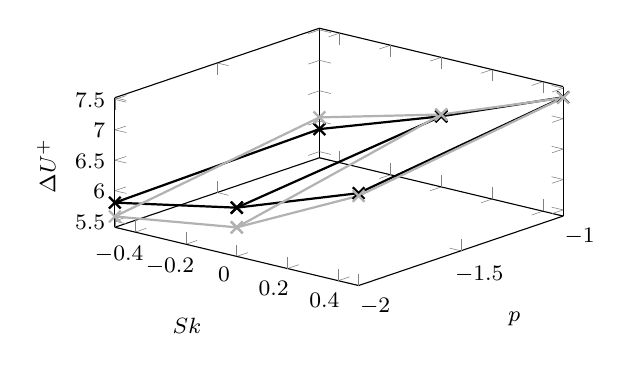
\begin{tikzpicture}[]
        \centering
        \begin{axis}[
        view={40}{35},
            ylabel={$p$},
            xlabel={$Sk$},
			zlabel={$\Delta U^+$},
			ztick={5.5,6,6.5,7,7.5},
            %ymin=0, ymax=1,
            width=.6\textwidth,
            height=.4\textwidth,
            label style={font=\footnotesize},
            tick label style={font=\footnotesize}
            ]
 %           \addplot3 [
%            blue,dashed,thick,no marks
%            ]
%            coordinates{
%            (0,-2,6.326)			%
%			(0.48,-2,6.994)%
%			(0.48,-1,7.336)
%			(0,-1,6.656)
%			(-0.48,-1,6.096)
%			(-0.48,-2,5.789)
 %           (0,-2,6.326)
%			};
%			\addplot3 [
 %5           red,dashed,thick, no marks
  %          ]
   %         coordinates{
    %        
    % 5       (0,-2,5.912)
	%		(0.48,-2,6.607)
	%		(0.48,-1,7.262)
	%5		(0,-1,6.530)
	%5		(-0.48,-1,6.075)
	%		(-0.48,-2,5.458)
	%5		(0,-2,5.912)
     %       };
                        \addplot3 [
            black,mark=x,thick, mark size=3pt
            ]
            coordinates{
            (0,-2,6.20)			
			(0.48,-2,6.9176)
			(0.48,-1,7.3502)
			(0,-1,6.56)
			(-0.48,-1,5.87)
			(-0.48,-2,5.8034)
            (0,-2,6.20)
			};
			\addplot3 [
            gray!60,mark=x,thick, mark size=3pt
            ]
            coordinates{
            
            (0,-2,5.8764)
			(0.48,-2,6.8720)
			(0.48,-1,7.3415)
			(0,-1,6.5891)
			(-0.48,-1,6.0625)
			(-0.48,-2,5.5765)
			(0,-2,5.8764)
            };
                                    \addplot3 [
            black,mark=x,thick, mark size=3pt
            ]
            coordinates{
            (0,-2,6.20)			
			(0,-1,6.56)
			};
			\addplot3 [
            gray!60,mark=x,thick, mark size=3pt
            ]
            coordinates{
            (0,-2,5.8764)
			(0,-1,6.5891)
            };
        \end{axis}
        \end{tikzpicture}
    \caption{$\Delta U^+$ prediction from minimal channels, black: $\lambda_0=0.8H$, gray: $\lambda_0=1.6H$}
    \label{fig-3d}
\end{figure}
%\begin{figure}
%\centering
    %        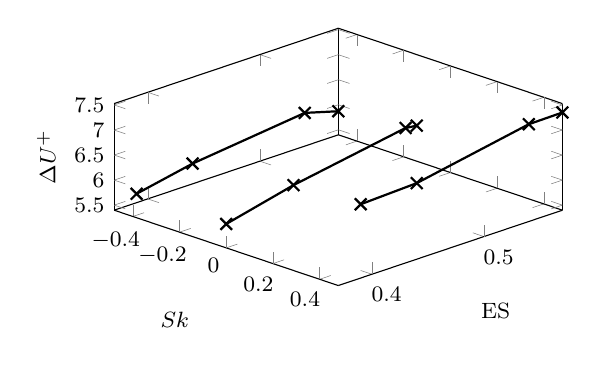
\begin{tikzpicture}[]
        \centering
        \begin{axis}[
        view={45}{45},
            ylabel={ES},
            xlabel={$Sk$},
			zlabel={$\Delta U^+$},
			ztick={5.5,6,6.5,7,7.5},
            %ymin=0, ymax=1,
            width=.6\textwidth,
            height=.4\textwidth,
            label style={font=\footnotesize},
            tick label style={font=\footnotesize}
            ]

                        \addplot3 [
            black,mark=x,thick, mark size=3pt
            ]
            coordinates{
			(0.48,0.39,6.8720)
			(0.48,0.44,6.9176)
			(0.48,0.54,7.3415)
			(0.48,0.57,7.3502)
			};
			\addplot3 [
            black,mark=x,thick, mark size=3pt
            ]
            coordinates{
            (0,0.37,5.8764)
            (0,0.43,6.20)
            (0,0.53,6.5891)
            (0,0.54,6.56)
            };
            
            
            
                                   \addplot3 [
            black,mark=x,thick, mark size=3pt
            ]
            coordinates{
			(-0.48,0.57,5.87)
			(-0.48,0.54,6.0625)
			(-0.48,0.44,5.8034)
			(-0.48,0.39,5.5765)
			};
        \end{axis}
        \end{tikzpicture}
    %\caption{$\Delta U^+$ prediction from minimal channels, black: $\lambda_0=0.8H$, gray: $\lambda_0=1.6H$}
%    \label{fig-3d}
%\end{figure}
\begin{figure}
\centering
            \begin{tikzpicture}[scale=0.85]
        \centering
        \begin{axis}[
            ylabel={$\Delta U^+$},
            xlabel={ES},
            ymin=0, ymax=12,
			xmax=0.9,
			xmin=0,
            width=.6\textwidth,
            height=.5\textwidth,
            label style={font=\footnotesize},
            legend style={font=\tiny,anchor=south east},
                        legend pos=south east,
            tick label style={font=\footnotesize}
            ]
			\addplot [
            black,only marks,thick,mark=o,
            ]
            coordinates{
            (0.57, 7.35)
            (0.54, 7.34)
            (0.44,6.92)
            (0.39,6.87)
            };
			\addlegendentry{$Sk=0.48$}
						\addplot [
            black!60,only marks,thick,mark=o,
            ]
            coordinates{
            (0.54,6.56)
            (0.53,6.59)
            (0.43,6.20)
            (0.37,5.88)
            };
			\addlegendentry{$Sk=0$}
			\addplot [
            black!30,only marks,thick,mark=o,
            ]
            coordinates{
            (0.57,5.87)
            (0.54,6.06)
            (0.44,5.80)
            (0.39,5.58)
            };
			\addlegendentry{$Sk=-0.48$}
						\addplot [
            black,only marks,thick,mark=*,
            ]
            coordinates{
            (0.041708,0.5762)
            (0.049156,0.7582)
            (0.0571,1.658)
            (0.063059,2.8307)
            (0.083416,3.249)
            (0.100298,4.246)
            (0.144489,6.3488)
            (0.147964,7.6226)
            (0.206058,8.1887)
            (0.298411,9.5029)
            (0.381827,10.1095)
            (0.550149,10.4431)
            (0.764151,10.2915)
            };
			\addlegendentry{~\citet{napoli_armenio_demarchis_2008}, $Re_\tau\approx395$}
				\addplot [
            gray!50,dashed,thick,
            ]
            coordinates{
(0.35,0)
(0.35,12)
            };
            				\addplot [
            gray!50,dashed,thick,
            ]
            coordinates{
(0.30,0)
(0.30,12)
            };
                \node[right] at (0.35,11) {\footnotesize{Roughness regime}};
                                \node[left] at (0.3,11) {\footnotesize{Waviness regime}};
        \end{axis}
        \end{tikzpicture}
    \caption{$\Delta U^+$ as a function of ES. The distinction between waviness and roughness roughness regimes as suggested by~\cite{Schultz2009} is indicated by vertical dashed lines.}
    \label{fig:DUES}
\end{figure}
So far we have discussed the effect of three parameters directly prescribed in the present work, i.e. $Sk$, $p$ and $\lambda_0$. ES is another roughness metric, which is widely discussed in the literature and used in roughness correlations. Even though ES is not explicitly prescribed in the present work, it is indirectly varied due to variation of other parameters. ES is particularly controlled by the two PS parameters $p$ and $\lambda_0$, which means that by varying these two parameters we implicitly study the effect of ES on the roughness function. In figure~\ref{fig:DUES} the correlation of $\Delta U^+$ and ES can be directly observed for the present data.
It is observed, that for all values of $Sk$, $\Delta U^+$ increases with ES. The slight drop of the last data point for Gaussian and negatively skewed roughness is likely due to the skimming effect of 'pit-dominant' surface with rapid surface sinking illustrated by the high ES.

Since all the present roughness topographies have an ES$>0.35$ they can be considered as roughness and not waviness surfaces according to the classification by~\citet{flack2010}. It is previously shown, e.g. by~\citep{napoli_armenio_demarchis_2008}, that roughness function only increases moderately with ES in this range, which agrees well with the presently observed trend.
As a reference, the data obtained at $Re_\tau\approx395$ by~\citet{napoli_armenio_demarchis_2008} are plotted in the same figure, in which irregular roughness are represented by superposition of different sinusoidal waves with random amplitude.
It is observed in the figure that, although the trend of $\Delta U^+$ with ES is similar in the present and the reference data, there are large offset between different groups of data points. It indicates that (obviously) roughness function is not uniquely determined by ES.



\subsubsection{Zero-plane displacement}
\begin{figure}
    \centering
            \begin{tikzpicture}[]
        \centering
        \begin{axis}[
            ylabel={$\Xi=(y-d)^+\frac{du^+}{dy^+}$},
            xlabel={$(y-d)^+$},
            ymin=0, ymax=8,
			xmin=1,xmax=500,
            width=.5\textwidth,
            height=.4\textwidth,
			xmode=log,
            legend style={font=\tiny,anchor=north west},
                        legend pos=north west,
            label style={font=\footnotesize},
            tick label style={font=\footnotesize}
            ]
            \addplot [
            black,solid,thick,
            ]
            table [x=X, y=Y,col sep=comma]{CSV/diagF1.csv};
                        \addlegendentry{$F-500$}
                        \addplot [
            black!60,solid,thick,
            ]
            table [x=X, y=Y,col sep=comma]{CSV/diagM11.csv};
                        \addlegendentry{$M1-500$}
                        \addplot [
            black!20,solid,thick,
            ]
            table [x=X, y=Y,col sep=comma]{CSV/diagM21.csv};
            \addlegendentry{$M2-500$}
                        			            \addplot [
            black,dashed,thick,
            ]
            coordinates{
            (80,-5)
            (80,10)
            };
                        \addlegendentry{Critical height $y_c$}
                        \addplot [
            black,solid,thick,
            ]
            table [x=X, y=Y,col sep=comma]{CSV/diagF2.csv};
                        \addplot [
            black!60,solid,thick,
            ]
            table [x=X, y=Y,col sep=comma]{CSV/diagM12.csv};
                        \addplot [
            black!20,solid,thick,
            ]
            table [x=X, y=Y,col sep=comma]{CSV/diagM22.csv};
                                    \addplot [
            black,solid,thick,
            ]
            table [x=X, y=Y,col sep=comma]{CSV/diagF3.csv};
                        \addplot [
            black!60,solid,thick,
            ]
            table [x=X, y=Y,col sep=comma]{CSV/diagM13.csv};
                        \addplot [
            black!20,solid,thick,
            ]
            table [x=X, y=Y,col sep=comma]{CSV/diagM23.csv};
                                    \addplot [
            black,solid,thick,
            ]
            table [x=X, y=Y,col sep=comma]{CSV/diagF4.csv};
                        \addplot [
            black!60,solid,thick,
            ]
            table [x=X, y=Y,col sep=comma]{CSV/diagM14.csv};
                        \addplot [
            black!20,solid,thick,
            ]
            table [x=X, y=Y,col sep=comma]{CSV/diagM24.csv};
                                    \addplot [
            black,solid,thick,
            ]
            table [x=X, y=Y,col sep=comma]{CSV/diagF5.csv};
                        \addplot [
            black!60,solid,thick,
            ]
            table [x=X, y=Y,col sep=comma]{CSV/diagM15.csv};
                        \addplot [
            black!20,solid,thick,
            ]
            table [x=X, y=Y,col sep=comma]{CSV/diagM25.csv};
                                    \addplot [
            black,solid,thick,
            ]
            table [x=X, y=Y,col sep=comma]{CSV/diagF6.csv};
                        \addplot [
            black!60,solid,thick,
            ]
            table [x=X, y=Y,col sep=comma]{CSV/diagM16.csv};
                        \addplot [
            black!20,solid,thick,
            ]
            table [x=X, y=Y,col sep=comma]{CSV/diagM26.csv};
                                    \addplot [
            black,solid,thick,
            ]
            table [x=X, y=Y,col sep=comma]{CSV/diagF7.csv};
                        \addplot [
            black!60,solid,thick,
            ]
            table [x=X, y=Y,col sep=comma]{CSV/diagM17.csv};
                                    \addplot [
            black,solid,thick,
            ]
            table [x=X, y=Y,col sep=comma]{CSV/diagF8.csv};
                        \addplot [
            black!60,solid,thick,
            ]
            table [x=X, y=Y,col sep=comma]{CSV/diagM18.csv};
                                    \addplot [
            black,solid,thick,
            ]
            table [x=X, y=Y,col sep=comma]{CSV/diagF9.csv};
                        \addplot [
            black!60,solid,thick,
            ]
            table [x=X, y=Y,col sep=comma]{CSV/diagM19.csv};
            
                        			            \addplot [
            black,dashed,thick,
            ]
            coordinates{
            (160,-5)
            (160,10)
            };
            \draw [dashdotted,black] (1,2.5) -- (500,2.5);
            
            
            
            
            
        \end{axis}
        \end{tikzpicture}
    \caption{Log-law diagnostic function, horizontal dash-dotted line represents $\Xi=2.5$, vertical dashed lines shows the critical height $y^+_c=80$, $160$ for $M$2-500 and $M$1-500, respectively.}
    \label{diag}
\end{figure}
\begin{figure}
    \centering
    \centering
                \begin{tikzpicture}[]
        \centering
        \begin{axis}[
            xlabel={ES},
			ylabel={$d/k$},
		%	ztick={5.5,6,6.5,7,7.5},
            ymin=0.6,ymax=1.2,
            width=.5\textwidth,
            height=.4\textwidth,
            label style={font=\footnotesize},
            tick label style={font=\footnotesize},
                        legend style={font=\tiny,anchor=south east},
                        legend pos=south east,
            ]

                        \addplot [
            black,mark=x,thick, mark size=3pt
            ]
            coordinates{
            (0.39,38.02/50)
			(0.44,40.02/50)
			(0.54,40.62/50)
			(0.57,40.87/50)
			};
			            \addlegendentry{$Sk=0.48$}
			\addplot [
            black!60,mark=x,thick, mark size=3pt
            ]
            coordinates{
            (0.37,44.82/50)
            (0.43,45.62/50)
			(0.53,47.29/50)
			(0.54,47.47/50)
            };
            			            \addlegendentry{$Sk=0$}
             \addplot [
            black!20,mark=x,thick, mark size=3pt
            ]
            coordinates{
			(0.39,50.38/50)
			(0.44,52.45/50)
			(0.54,53.03/50)
			(0.57,53.23/50)
			};
            			            \addlegendentry{$Sk=-0.48$}
        \end{axis}
        \end{tikzpicture}
    \caption{$d$ predictions as a function of ES, grouped by $Sk$.}
    \label{plot2dk}
\end{figure}
 As discussed before due to the rough structures, the logarithmic layer of the flow is shifted upwards to the fluid. Thus, the origin of wall-normal coordinate cannot be defined \textit{a priori}.
As a result it is necessary to use a physically justified virtual origin for the logarithmic law of the wall. 
The virtual origin lies above the $y=0$ plane at a distance equal to zero-plane displacement $d$.
The definition of the virtual wall in the present work follows the method proposed by~\citet{jackson_1981}.
In order to investigate if the present choice of virtual wall leads to a satisfactory logarithmic behavior, diagnostic functions $\Xi=(y-d)^+\mathrm{d}u^+/\mathrm{d}y^+$ are shown in figure~\ref{diag}.
The constant value of $\Xi\approx2.5$ is expected in the logarithmic region.
%In logarithmic layer, it is widely reported that $\Xi\approx2.5$.
One should note that, due to the limited extend of `healthy turbulence' in minimal channels, logarithmic profile is only expected to exist under the critical height $y_c$.
Hence, it is observed that with decreasing the channel size, the diagnostic functions deviate from those of the full channel simulations beyond $y_c$. 
The value of zero-plane displacement $d/k$ are documented in table~\ref{ResultAll}.
To summarize the effect of roughness topography on zero-plane displacement $d/k$ is plotted as a function of  effective slope ES in figure~\ref{plot2dk}, while the data points are grouped by $Sk$.
It can be observed that the value of $d/k$ increases with an increase in ES and a decrease in $Sk$, while the skewness effect is more dominant.
Have to mention that for the cases with negative $Sk$ $1<d/k<k_\text{t}/k$ so that the zero plane displacement is still below the maximum roughness height.
%As one can observe from the results, the zero-plane shift is a function of both the height and spatial distribution:
%The zero-plane is pushed higher with increasing occupation of solid wall structure - as reflected by the melt-down height $k_{md}$ - due to the different prescription of skewness.
%As the the rough surface becomes steeper - as reflected by the effective slope ES- the zero plane is shifted higher.
%The distance between $d$ and $k_{md}$ normalized by $k_{rms}$ for all cases are plotted in figure~\ref{plot3dd}(b) as a function of Sk and $p$. 
%Over past few decades, researchers have been trying to relate $d$ to roughness topographical properties~~\cite{chan-braun_garcia-villalba_uhlmann_2011,hopkins2011,Raupach1992}, for example in urban aerodynamics, models are developed to relate $d$ normalized with mean building height $h_m$ to the surface properties.
%For irregular roughness, as a substitution to $h_m$, the roughness height $k_{rms}$ is used for normalization.
%Analogous to these studies, we seek correlation of the separation factor $\frac{d-k_{md}}{k_{rms}}$ with roughness topographical properties.
%The roughness parameters $k_t$ and $L_x^{corr}$ are chosen to build the correlation as representation of both height and spatial distribution, respectively.
%The peak-to-trough height $k_t$ is transformed to the scale of distance by subtracting melt-down height $k_{md}$.
%The final form of the correlation writes:
%\begin{equation}
%    \frac{d-k_{md}}{k_{rms}}=0.1645\frac{k_t-k_{md}}{k_{rms}}e^{-0.025\frac{L_x^{corr}}{k_{rms}}}+1.1293
%\end{equation}
%The predicted separation factor corresponding to each topographies are plotted in figure~\ref{plot3dd}(b) with circles.
%Root mean squared percentage error (RMSPE) is 6.4\%.


%\begin{figure}[ht]
%\begin{subfigure}[t]{0.5\linewidth}
%\centering
%\input{DP14}
%\caption{P14}
%\end{subfigure}\hfill%
%\begin{subfigure}[t]{0.5\linewidth}
%\centering
%\input{DP24}
%\caption{P24}
%\end{subfigure}
%\begin{subfigure}[t]{0.5\linewidth}
%\centering
%\input{DP18}
%\caption{P28}
%\end{subfigure}\hfill%
%\begin{subfigure}[t]{0.5\linewidth}
%\centering
%\input{DP28}
%\caption{P28}
%\end{subfigure}
%\begin{subfigure}[t]{0.5\linewidth}
%\centering
%\input{DG14}
%\caption{G14}
%\end{subfigure}\hfill%
%\begin{subfigure}[t]{0.5\linewidth}
%\centering
%\input{DG24}
%\caption{G24}
%\end{subfigure}
%\begin{subfigure}[t]{0.5\linewidth}
%\centering
%\begin{tikzpicture}
\begin{axis}[
		xlabel={$L_x$, [H]},
		ylabel={$k$, [H]},
		xmin=0,xmax=2.4,
		ymin=0,ymax=0.12,
		%y dir=reverse,
		clip=true,
		set layers,
		clip mode=individual,
	    height=0.3\linewidth,
		width=.9\linewidth,
		axis x line*=bottom,
		axis y line*=left,
		xtick={0,0.4,...,2.4},
		ytick={0,0.04,...,0.12},
		label style={font=\footnotesize},
		yticklabel style={/pgf/number format/fixed},
		tick label style={font=\footnotesize},
		at={(0,0.35\linewidth)}
	]
	\centering
    \addplot+[ name path=A,
            red,solid,thick,mark=none
            ]
            table [x=X, y=Y,col sep=comma]{CSV/G18H.csv};
    \path[name path=B,black,mark=none] (axis cs:0,0) -- (axis cs:2.4,0);
    \addplot[gray,mark=none] fill between[of=A and B];
    							\addplot [
            gray,thick,dashed,mark=square,
            ]
            coordinates{
            (-0.5, 47.29/500)
            (3, 47.29/500)
            };
                							\addplot [
                        black,thick,solid,mark=square,
            ]
            coordinates{
            (-0.5, 0.061)
            (3, 0.061)
            };
\end{axis}
\end{tikzpicture}
%\caption{G18}
%\end{subfigure}\hfill%
%\begin{subfigure}[t]{0.5\linewidth}
%\centering
%\input{DG28}
%\caption{G28}
%\end{subfigure}
%\begin{subfigure}[t]{0.5\linewidth}
%\centering
%\input{DN14}
%\caption{N14}
%\end{subfigure}\hfill%
%\begin{subfigure}[t]{0.5\linewidth}
%\centering
%\input{DN24}
%\caption{N24}
%\end{subfigure}
%\begin{subfigure}[t]{0.5\linewidth}
%\centering
%\input{DN18}
%\caption{N18}
%\end{subfigure}\hfill%
%\begin{subfigure}[t]{0.5\linewidth}
%\centering
%\input{DN28}
%\caption{N28}
%\end{subfigure}
%\caption{Sketch of the zero-plane displacement $d$ and melt-down %height $k_{md}$.(\full: $k_{md}$, \dashed: $d$)}
%\label{SD}
%\end{figure}
%\begin{figure}
    %\centering
    %\centering
        %        \begin{tikzpicture}[]
        \centering
        \begin{axis}[
        view={40}{35},
            ylabel={$p$},
            xlabel={\textit{Sk}},
			zlabel={$d/k$},
		%	ztick={5.5,6,6.5,7,7.5},
            %zmin=0.06,% ymax=1,
            width=.6\textwidth,
            height=.4\textwidth,
            label style={font=\footnotesize},
            tick label style={font=\footnotesize}
            ]

                        \addplot3 [
            black,mark=x,thick, mark size=3pt
            ]
            coordinates{
            (0,-2,45.62/50)			
			(0.48,-2,40.02/50)
			(0.48,-1,40.87/50)
			(0,-1,47.47/50)
			(-0.48,-1,53.23/50)
			(-0.48,-2,52.45/50)
            (0,-2,45.62/50)
			};
			\addplot3 [
            gray,mark=x,thick, mark size=3pt
            ]
            coordinates{
            
            (0,-2,44.82/50)
			(0.48,-2,38.02/50)
			(0.48,-1,40.62/50)
			(0,-1,47.29/50)
			(-0.48,-1,53.03/50)
			(-0.48,-2,50.38/50)
			(0,-2,44.82/50)
            };
            
                                                %\addplot3 [
            %red,mark=o,thick, mark size=3pt
            %]
            %coordinates{
            %(0,-2,1.58018*0.02+0.061)			
			%(0.48,-2,1.6769*0.02+0.046)
			%(0.48,-1,1.67396*0.02+0.046)
			%(0,-1,1.57652*0.02+0.061)
			%(-0.48,-1,1.45811*0.02+0.074)
			%(-0.48,-2,1.45994*0.02+0.074)
            %(0,-2,1.58018*0.02+0.061)
			%};
			%\addplot3 [
            %%red,mark=o,dotted,thick, mark size=3pt
            %]
            %coordinates{
            
        %    (0,-2,1.51138*0.02+0.061)
	%		(0.48,-2,1.6007*0.02+0.046)
	%		(0.48,-1,1.68346*0.02+0.046)
	%		(0,-1,1.58295*0.02+0.061)
	%		(-0.48,-1,1.46401*0.02+0.074)
	%		(-0.48,-2,1.41258*0.02+0.074)
	%		(0,-2,1.51138*0.02+0.061)
     %       };
        \end{axis}
        \end{tikzpicture}
    %\caption{$d$ prediction from minimal channels, black: $\lambda_0=0.8H$, gray: $\lambda_0=1.6H$.}
    %\label{plot3dd}
%\end{figure}
%\begin{figure}
    %\centering
    %\centering
        %        \begin{tikzpicture}[]
        \centering
        \begin{axis}[
        view={40}{35},
            ylabel={ES},
            xlabel={\textit{Sk}},
			zlabel={$d/k$},
		%	ztick={5.5,6,6.5,7,7.5},
            %zmin=0.06,% ymax=1,
            width=.6\textwidth,
            height=.4\textwidth,
            label style={font=\footnotesize},
            tick label style={font=\footnotesize}
            ]

                        \addplot3 [
            black,mark=x,thick, mark size=3pt
            ]
            coordinates{
            (0.48,0.39,38.02/50)
			(0.48,0.44,40.02/50)
			(0.48,0.54,40.62/50)
			(0.48,0.57,40.87/50)
			};
			\addplot3 [
            black,mark=x,thick, mark size=3pt
            ]
            coordinates{
            (0,0.37,44.82/50)
            (0,0.43,45.62/50)
			(0,0.53,47.29/50)
			(0,0.54,47.47/50)
            };
             \addplot3 [
            black,mark=x,thick, mark size=3pt
            ]
            coordinates{
			(-0.48,0.39,50.38/50)
			(-0.48,0.44,52.45/50)
			(-0.48,0.54,53.03/50)
			(-0.48,0.57,53.23/50)
			};

        \end{axis}
        \end{tikzpicture}
    %\caption{$d$ prediction from minimal channels, black: $\lambda_0=0.8H$, gray: $\lambda_0=1.6H$.}
    %\label{plot3dk}
%\end{figure}

%\begin{figure}
%    \centering
%    \begin{tikzpicture}[]
        \centering
        \begin{axis}[
        grid style={line width=.1pt, draw=gray!10},major grid style={line width=.2pt,draw=gray!50},
            ylabel={Zero-plane displacement $d^+$},
            xlabel={Melt-down height $k_{md}^+$},
            ymin=0, ymax=3,
			xmax=0.08*500,
			xmin=0.04*500,
			%xtick={-2,-1.5,...,-0.4},
            width=.8\linewidth,
            height=.6\linewidth,
            label style={font=\footnotesize},
			legend style={font=\tiny,at={(0,1)},anchor=north west},
			xticklabel style={/pgf/number format/fixed},
			yticklabel style={/pgf/number format/fixed},
            tick label style={font=\footnotesize}
            ]
			\addplot [
            black,mark=o,
            ]
            coordinates{
            (0.046*500,40.87/23)
            (0.061*500,47.47/30.5)
            (0.074*500,53.23/37)
            };
        			\addlegendentry{$p=-1$, $\lambda_0=0.4H$}
        			\addplot [
            black,mark=square,
            ]
            coordinates{
            (0.046*500,40.02/23)
            (0.061*500,45.62/30.5)
            (0.074*500,52.45/37)
            };
                			\addlegendentry{$p=-2$, $\lambda_0=0.4H$}
        			\addplot [
            black,mark=x,
            ]
            coordinates{
            (0.046*500,40.62/23)
            (0.061*500,47.29/30.5)
            (0.074*500,53.03/37)
            };
                    			\addlegendentry{$p=-1$, $\lambda_0=0.8H$}
                    			\addplot [
            black,mark=triangle,
            ]
            coordinates{
            (0.046*500,38.02/23)
            (0.061*500,44.82/30.5)
            (0.074*500,50.38/37)
            };
                    			\addlegendentry{$p=-2$, $\lambda_0=0.8H$}
        \end{axis}
        \end{tikzpicture}
%    \caption{Caption}
%    \label{fig:my_label}
%\end{figure}

\subsection{Assessment of existing roughness correlations}
\label{sec:corr}
In this section, results from previously introduced topographies at $Re_\tau\approx500$ are used to assess some of the existing roughness correlations.
 As a matter of fact, existing roughness correlations are developed based on a limited number of data points covering a certain region of the parameter space~\citep{Chung2021annrev}. In this section, we are particularly interested to shed light on the generalization of these correlations outside their original parameter space, which is a key for a correlation to work across a wide range of rough surfaces encountered in different applications. There are in general two types of roughness correlations in literature, those directly predicting the equivalent sand-grain roughness $k_s$ and those predicting the roughness function $\Delta U^+$. The latter group is more suitable for the transitionally rough regime since $k_s$ is essentially defined when the flow is fully rough. In the following we first assess three correlations  (Eqn.~\ref{Chan1}, Eqn.~\ref{Chan2} and Eqn.~\ref{thakkar}) developed based on transitionally and fully rough data and then examine two correlations (Eqns~\ref{forooghi} and~\ref{flack}) specifically developed for the fully-rough regime.
It was shown in the previous sections that a fully rough regime for the surfaces under investigation is likely reached at about $\Delta U^+>6$. However, in the present section we calculate the equivalent roughness height based on $\Delta U^+$ for all cases, including those with values of roughness function smaller but close to 6. It must however be kept in mind that $k_s$ is only a relevant quantity in the fully rough regime.
Figure~\ref{Cor2} visualizes the selected correlations, where parameter space covered by fitting data of each correlation is represented by a red frame. In each sub-figure the data points from the present work are depicted as symbols. Different symbol colors are used to make distinction between the data points lying inside and outside the fitting region. Here the parameter space is expressed in terms of the two widely used parameters $Sk$ and ES, even though they both may not explicitly appear as predictive parameters in all correlations.
 
Required roughness statistics of the present roughness topographies are listed in Table~\ref{tab:SumOfCase}.
First we examine the correlation proposed by~\citet{chan2015}, which is based on 3D sinusoidal roughness data in both transitionally and fully rough regimes. These authors proposed expressions for $\Delta U^+$ and $k_s$ as follows. 
 \begin{equation}
     \Delta U^+=\frac{1}{\kappa}\text{log}(k_a^+)+1.12 \text{log}(\text{ES})+1.47~,
     \label{Chan1}
 \end{equation}
 \begin{equation}
     k_s=7.3k_a\text{ES}^{0.45}~.
     \label{Chan2}
\end{equation}
 %It is noticeable that the fitting data which the authors used for developing the correlation has a range of $Sk>0$, $0<ES<1$ while $1\leq k_a^+\leq40$.
 We visualized only one of these two related correlations in figure~\ref{Cor2} (a). %, where color indicates the prediction value, symbols represent the data points from present work. 
 The data points from the present work locate in the range of fitting data except for the topographies with $Sk<0$.
 Obviously, since $Sk$ is not used as a predictive parameter in these correlations, they returns same predictions for different values of $Sk$.
 
 ~\citet{Thakkar2017}, developed a correlation based on a roughness parameter $\lambda_T$ including a wider range of primary topographical parameters. Their correlation is developed in transitionally rough regime, thus only $\Delta U^+$ is predicted.
 In this correlation, $\Delta U^+$ is linearly related to $\lambda_T$:
  \begin{subequations}
         \begin{equation}
         \Delta U^+ = \alpha_T\lambda_T+\beta_T~, \text{}
 \end{equation}
 \begin{equation}
         \lambda_T=\text{ln}\bigl(\frac{S_f}{S} \bigr)\bigl[1+0.09\text{ln}\bigl(\frac{L_x^{\text{corr}}}{k_{\text{t},5\times5}} \bigr)\bigr]\bigl(\frac{4k_{\text{rms}}}{k_{\text{t},5\times5}}\bigr)^{-0.44}e^{(-0.074Sk)}~,
         \end{equation}
         \label{thakkar}
 \end{subequations}
 where $\alpha_T=1.4699$ and $\beta_T=8.0394$ represent empirical parameters.
 $S_f/S$ is the ratio of the total frontal projected area and wall-normal projected area of the roughness.
 $L_x^{\text{corr}}$ is the correlation length of roughness, at which length scale auto-correlation of roughness drops to 0.2. 
 $k_{\text{t},5\times5}$ is the peak-to-trough height averaged over $5\times5$ uniform subsets of the surface.%, for all present topographies, this value coincident with $k_t$. % due to the PDF cutoff described in~\cref{sec:cases}.
 %Therefore, both spatial distribution as well as the height distribution information of roughness are involved in the model.
 The prediction of $\Delta U^+$ by this correlation is shown in figure~\ref{Cor2}(b) as a function of $Sk$ and ES. 

 %Roughness parameters despite $Sk$ and $ES$ are chosen to be the constant that comparable with present roughness data set.
 
 It can be observed from figure~\ref{Cor2}(b), that all the data from the present work locate outside of the fitting data in terms of $Sk$ and ES.
% Have to mention that this work serves merely as a contribution to the characterization of roughness physical characterization, roughness function $\Delta U^+$ can not be uniquely determined by the roughness physical properties but also with the flow configurations, i.e. $Re_\tau$.
 %In order to evaluate the parametrisation model $\lambda_T$ with the present data set, empirical parameters $\alpha_T$ and $\beta_T$ are fitted from present results ($\alpha_T=1.2702$ and $\beta_T=8.5619$).
 %In the original work, surfaces have identical roughness height $k^+=30$, which is approximately comparable with present data set with $k^+=50$. Thus, $\alpha_T=1.4699$ and $\beta_T=8.0394$ proposed by these authors are also used for comparison.
% Slight differences in the parameters can be attributed to the varied flow configuration.
 Furthermore, two correlations specifically aimed at fully-rough regime are examined. These are the correlation by~\citet{10.1115/1.4037280}
 \begin{equation}
     k_s=k[0.67Sk^2+0.93Sk+1.3][1.07(1-e^{-3.5\text{ES}})]~,
     \label{forooghi}
 \end{equation}
and the one by~\citet{Flack2020},
 \begin{equation}
        \left\{
\begin{array}{ll}
      k_s=2.73k_{\text{rms}}(2+Sk)^{-0.45}~,& Sk<0~,\\
      k_s=2.11k_{\text{rms}}~,& Sk=0~,\\
      k_s=2.48k_{\text{rms}}(1+Sk)^{2.24}~,& Sk>0~. \\
\end{array} 
\right. 
\label{flack}
 \end{equation}
\\
\begin{figure}
    \centering
        \begin{subfigure}[t]{0.5\linewidth}
        \input{tikz/CorrChan_Ks}
    \caption{Eqn.~\ref{Chan2} by~\citet{chan2015}}
    \end{subfigure}\hfill%
        \begin{subfigure}[t]{.5\linewidth}
    
    \begin{tikzpicture}
\begin{axis}[view={0}{90},
		xlabel=$Sk$,
		ylabel=ES,
		%title=$\Delta U^+$,
		%colormap/parula,
		mesh/cols=50,
		height=.8\linewidth,
		width=.8\linewidth,
		colorbar,
				colorbar style={
				xlabel=$\Delta U^+$,
				xlabel shift = 10.5 pt,
		width=0.2cm
		}
		]
\addplot3 [surf,shader=interp]
  table[x=X, y=Z, z=Y, col sep=comma] {CSV/Thakkar_DU.csv};
  			            \addplot3 [
            black,only marks,mark=square, mark size=1.5pt
            ]
            coordinates{
            (0,0.54,1)			
			(0,0.52,1)
			(0,0.41,1)
			(0,0.36,1)
			(0.48,0.56,1)			
			(0.48,0.54,1)
			(0.48,0.42,1)
			(0.48,0.37,1)
			};
			  			            \addplot3 [
            black,only marks,mark=square, mark size=1.5pt
            ]
            coordinates{
			(-0.48,0.56,1)			
			(-0.48,0.54,1)
			(-0.48,0.42,1)
			(-0.48,0.37,1)			
			};
			\draw[color=red,thick] (-0.5, 0.06 ) rectangle (0.6,0.32);
			\node[red,right] at (axis cs: -0.150,0.2) {\tiny Fitting data};
\end{axis}
\end{tikzpicture}
    \caption{Eqn.~\ref{thakkar} by~\citet{Thakkar2017}.}   
    \end{subfigure}
    \centering
        \begin{subfigure}[t]{0.5\linewidth}
        \begin{tikzpicture}
\begin{axis}[view={0}{90},
		xlabel=$Sk$,
		ylabel=ES,
		%title=$k_s^+$,
		%colormap/parula,
		mesh/cols=50,
		height=.8\linewidth,
		width=.8\linewidth,
		colorbar,
				colorbar style={
				xlabel=$k_s^+$,
				xlabel shift = 10.5 pt,
		width=0.2cm
		}
		]
\addplot3 [surf,shader=interp]
  table[x=X, y=Z, z=Y, col sep=comma] {CSV/Forooghi.csv};
  			            \addplot3 [
            black,only marks,mark=square, mark size=1.5pt
            ]
            coordinates{

			(-0.48,0.56,1)			
			(-0.48,0.54,1)
			(-0.48,0.42,1)
			(-0.48,0.37,1)			
			};
  			            \addplot3 [
            red,only marks,mark=square, mark size=1.5pt
            ]
            coordinates{
            (0,0.54,1)			
			(0,0.52,1)
			(0,0.41,1)
			(0,0.36,1)
			(0.48,0.56,1)			
			(0.48,0.54,1)
			(0.48,0.42,1)
			(0.48,0.37,1)			
			};
			\draw[color=red,thick] (-0.35, 0.2 ) rectangle (0.68,0.89);
			\node[red,right] at (axis cs: -0.2,0.8) {\tiny Fitting data};
\end{axis}
\end{tikzpicture}
    \caption{Eqn.~\ref{forooghi} by~\citet{10.1115/1.4037280}}
    \end{subfigure}\hfill%
    \begin{subfigure}[t]{0.5\linewidth}
        \begin{tikzpicture}
\begin{axis}[view={0}{90},
		xlabel=$Sk$,
		ylabel=ES,
		%title=$k_s^+$,
		%colormap/parula,
		mesh/cols=50,
		height=.8\linewidth,
		width=.8\linewidth,
		colorbar,
				colorbar style={
				xlabel=$k_s^+$,
				xlabel shift = 10.5 pt,
		width=0.2cm
		}
		]
\addplot3 [surf,shader=interp]
  table[x=X, y=Z, z=Y, col sep=comma] {CSV/flack.csv};
  			            \addplot3 [
            black,only marks,mark=square, mark size=1.5pt
            ]
            coordinates{
            (0,0.54,1)			
			(0,0.52,1)
			(0.48,0.56,1)			
			(0.48,0.54,1)
			(-0.48,0.56,1)			
			(-0.48,0.54,1)		
			};
			  			            \addplot3 [
            red,only marks,mark=square, mark size=1.5pt
            ]
            coordinates{		
			(0,0.41,1)
			(0,0.36,1)			
			(0.48,0.42,1)
			(0.48,0.37,1)			
			(-0.48,0.42,1)
			(-0.48,0.37,1)			
			};
			\draw[color=red,thick] (-0.7, 0.19 ) rectangle (0.84,0.47);
			\node[red,right] at (axis cs: 0.1,0.25) {\tiny Fitting data};
\end{axis}
\end{tikzpicture}
    \caption{Eqn.~\ref{flack} by~\citet{Flack2020}}
    \end{subfigure}
    \caption{Predictive correlations of $k_s^+$ and $\Delta U^+$. Squares indicate data points from present work while red frame represents the fitting data from literature. $S_f/S=0.25$, $L_x^{\text{corr}}=0.08H$, $k_{\text{t}}=0.12H$, $k_{\text{rms}}=0.02H$, are chosen to be comparable with the present roughness dataset. }
    \label{Cor2}
\end{figure}
\begin{table}
    \centering
                \begin{tabular}{c c c c }
         Topography& $\Delta U^+_{\text{DNS}}$ &$\Delta U^+_{\text{Eqn.\ref{Chan1}}}$& $\Delta U^+_{\text{Eqn.\ref{thakkar}}}$  \\[3pt]
         $P14$ & 7.33&6.06 &6.09\\
         $P18$&7.23&6.00&6.04\\
         $P24$&6.99&5.77&5.51\\
         $P28$&6.57&5.64&5.19\\[3pt]
         $G14$ &6.67&5.85 &5.89\\
         $G18$&6.56&5.83&5.82\\
         $G24$&6.30&5.60&5.27\\
         $G28$&5.94&5.43&4.92\\[3pt]
         $N14$ &6.14& 6.06 &5.94\\
        $ N18$&6.09&6.00&5.89\\
         $N24$&5.82&5.77&5.32\\
         $N28$&5.51&5.64&4.98\\
         
    \end{tabular}
            \caption{Prediction of $\Delta U^+$ by Chan \textit{et al.} and Thakkar \textit{et al.}}
    \label{tab:CorDU}
\end{table}

\begin{table}
    \centering
                \begin{tabular}{c c c c c}
         Topography& $k^+_{s,\text{DNS}}$ &$k^+_{s,\text{Eqn.\ref{Chan2}}}$& $k^+_{s,\text{Eqn.\ref{flack}}}$&$k^+_{s,\text{Eqn.\ref{forooghi}}}$  \\[3pt]
         $P14$ &69.69&48.18 &62.07&87.86\\
         $P18$&66.95&47.02&62.07&86.33\\
         $P24$&60.82&42.88&62.07&79.89\\
         $P28$&51.42&40.62&62.07&75.72\\[3pt]
         $G14$ &53.52&44.26 &21.10&59.04\\
         $G18$&51.21&43.89&21.10&58.67\\
         $G24$&46.15&39.95&21.10&54.11\\
         $G28$&39.96&37.33&21.10&50.50\\[3pt]
         $N14$ &43.29&48.18 &23.52&32.32\\
         $N18$&42.44&47.02&23.52&31.76\\
         $N24$&38.09&42.88&23.52&29.39\\
         $N28$&33.65&40.62&23.52&27.86\\
    \end{tabular}
            \caption{Prediction of $k_s$ by Chan \textit{et al.}, Flack \textit{et al.} and Forooghi \textit{et al.}}
    \label{tab:Corks}
\end{table}
\begin{figure}
    \centering
    \begin{subfigure}[t]{\linewidth}
        \centering
                \begin{tikzpicture}[]
        \centering
        \begin{axis}[
            ylabel={$\Delta U_{\text{Eqn}}^+/\Delta U_{\text{DNS}}^+$},
            xlabel={$\Delta U_{\text{DNS}}^+$},
            ymin=0, ymax=2,
			xmax=8,
			xmin=5,
			%xtick={-2,-1.5,...,-0.4},
            width=.6\textwidth,
            height=.5\textwidth,
            label style={font=\footnotesize},
            legend style={font=\tiny,anchor=south east},
                        legend pos=south east,
            tick label style={font=\footnotesize}
            ]
            \fill[color=green!20,opacity=20] (0,1.09) -- (10,1.09) -- (10,0.87) -- (0,0.87) -- cycle;
            \fill[color=green!50,opacity=50] (0,1.07) -- (10,1.07) -- (10,0.92) -- (0,0.92) -- cycle;
            \fill[color=green!100,opacity=100] (0,1.03) -- (10,1.03) -- (10,0.96) -- (0,0.96) -- cycle;

			\addplot [
            black,only marks,mark=triangle,
            ]
            coordinates{
            (6.14,6.0601/6.14)
            (6.09,5.9995/6.09)
            (5.82,5.7702/5.82)
            (5.51,5.6351/5.51)
            };
			\addlegendentry{Eqn.~\ref{Chan1}}
						\addplot [
            black,only marks,mark=star,
            ]
            coordinates{
            (7.33,6.09/7.33)
            (7.23,6.04/7.23)
            (6.99,5.51/6.99)
            (6.57,5.19/6.57)
            (6.67,5.89/6.67)
            (6.56,5.82/6.56)
            (6.30,5.27/6.30)
            (5.94,4.92/5.94)
            (6.14,5.94/6.14)
            (6.09,5.89/6.09)
            (5.82,5.32/5.82)
            (5.51,4.98/5.51)
            };
%\addlegendentry{Eqn.~\ref{thakkar}, $\alpha_T=1.2702$, $\beta_T=8.5619$}
		%	\addlegendentry{Eqn.~\ref{thakkar}}
%												\addplot [
%            red,only marks,mark=star,
%            ]
%            coordinates{
%            (7.33,6.87/7.33)
%            (7.23,6.38/7.23)
%            (6.99,6.83/6.99)
%            (6.57,6.10/6.57)
%            (6.67,6.70/6.67)
%            (6.56,6.17/6.56)
%            (6.30,6.64/6.30)
%            (5.94,5.87/5.94)
%            (6.14,6.75/6.14)
%%            (6.09,6.21/6.09)
 %           (5.82,6.70/5.82)
 %           (5.51,5.92/5.51)
 %           };
						\addlegendentry{Eqn.~\ref{thakkar}}
			
			
			
			
						\addplot [
            red,only marks,mark=triangle,
            ]
            coordinates{
            (6.67,5.8517/6.67)
            (6.56,5.8307/6.56)
            (6.30,5.5966/6.30)
            (5.94,5.4282/5.94)
            
            (7.33,6.0601/7.33)
            (7.23,5.9995/7.23)
            (6.99,5.7702/6.99)
            (6.57,5.6351/6.957)
            
            };
			

			
							\addplot [
            gray,thick,dashed,mark=square,
            ]
            coordinates{
            (6, 2.5)
            (6, -1)
            };
									\node[black,right] at (axis cs: 6,1.75) {\tiny Fully rough regime};
							\addplot [
            red,thick,mark=square,
            ]
            coordinates{
            (4, 1)
            (9, 1)
            };									           
        \end{axis}
        \end{tikzpicture}
    \end{subfigure}\hfill
    \begin{subfigure}[t]{\linewidth}
        \centering
            \begin{tikzpicture}[]
        \centering
        \begin{axis}[
            ylabel={$k_{s,\text{Eqn}}^+/k_{s,\text{DNS}}^+$},
            xlabel={$k_{s,\text{DNS}}^+$},
            ymin=0, ymax=2,
			xmax=110,
			xmin=20,
			%xtick={-2,-1.5,...,-0.4},
            width=.6\textwidth,
            height=.5\textwidth,
            label style={font=\footnotesize},
            legend style={font=\tiny,anchor=south east},
                        legend pos=south east,
            tick label style={font=\footnotesize}
            ]
			 \fill[color=green!20,opacity=20] (0,1.3) -- (200,1.3) -- (200,0.7) -- (0,0.7) -- cycle;
			 \fill[color=green!50,opacity=50] (0,1.2) -- (200,1.2) -- (200,0.8) -- (0,0.8) -- cycle;
			 \fill[color=green!100,opacity=100] (0,1.1) -- (200,1.1) -- (200,0.9) -- (0,0.9) -- cycle;

			\addplot [
            black,only marks,mark=triangle,
            ]
            coordinates{
                        (43.2934,48.1821/43.2934)
            (42.4361,47.0239/42.4361)
            (38.0918,42.8840/38.0918)
            (33.4265,40.6182/33.4265)                
            
            };
			\addlegendentry{Eqn.~\ref{Chan2}}
			\addplot [
            black,only marks,mark=square,
            ]
            coordinates{
            (53.5170,21.1/53.5170)
            (51.2133,21.1/51.2133)
            (69.6860,62.0685/69.6860)
            (66.9536,62.0685/66.9536)
                        (43.2934,23.5162/43.2934)
            (42.4361,23.5162/42.4361)
            };
			\addlegendentry{Eqn.~\ref{flack}}
			\addplot [
            black,only marks,mark=o,
            ]
            coordinates{
            (43.2934,32.3208/43.2934)
            (42.4361,31.7575/42.4361)
            (38.0918,29.3891/38.0918)
            (33.4265,27.8554/33.4265)  
            
            };
			\addlegendentry{Eqn.~\ref{forooghi}}
	
	%						\addplot [
         %   black,only marks,mark=star,
         %   ]
         %   coordinates{
         %   (69.69,42.44/69.69)
         %   (66.95,41.60/66.95)
         %   (60.82,33.65/60.82)
         %   (51.42,29.61/51.42)
         %   (53.52,39.17/53.52)
         %   (51.21,38.09/51.21)
         %   (46.15,30.57/46.15)
         %   (39.96,26.58/39.96)
         %   (43.29,39.96/43.29)
         %   (42.44,39.17/42.44)
         %   (38.09,31.19/38.09)
         %   (33.65,27.22/33.65)
         %   };
		%	\addlegendentry{Eqn.~\ref{thakkar}~\cite{Thakkar2017}}
	
	
	
				\addplot [
            red,only marks,mark=triangle,
            ]
            coordinates{
                        (53.5170,44.2578/53.5170)
            (51.2133,43.8871/51.2133)
            (46.1548,39.9460/46.1548)
            (39.9648,37.3339/39.9648)
            
                        (69.6860,48.1821/69.6860)
            (66.9536,47.0239/66.9536)
            (60.8249,42.8840/60.8249)
            (51.4186,40.6182/51.4186)            
            
            };
	
			\addplot [
            red,only marks,mark=square,
            ]
            coordinates{
            (46.1548,21.1/46.1548)
            (39.9648,21.1/39.9648)

            (60.8249,62.0685/60.8249)
            (51.4186,62.0685/51.4186)           

            (38.0918,23.5162/38.0918)
            (33.4265,23.5162/33.4265)  
            };	
			\addplot [
            red,only marks,mark=o,
            ]
            coordinates{
                        (53.5170,59.0430/53.5170)
            (51.2133,58.6687/51.2133)
            (46.1548,54.1087/46.1548)
            (39.9648,50.5004/39.9648)
            
                        (69.6860,87.8597/69.6860)
            (66.9536,86.3284/66.9536)
            (60.8249,79.8904/60.8249)
            (51.4186,75.7211/51.4186)   
            };	
	
	
	
	
	
	
	
	
	
	
	
	
						\addplot [
            red,thick,solid,mark=square,
            ]
            coordinates{
            (0, 1)
            (201, 1)
            };
            						\addplot [
            gray,thick,dashed,mark=square,
            ]
            coordinates{
            (40.9356, 3)
            (40.9356, -1)
            };
			\node[red,right] at (axis cs: 90,1.05) {\tiny $\pm10\%$};
						\node[red,right] at (axis cs: 90,1.15) {\tiny $\pm20\%$};
									\node[red,right] at (axis cs: 90,1.25) {\tiny $\pm30\%$};
																		\node[black,right] at (axis cs: 40.9356,1.75) {\tiny Fully rough regime};
        \end{axis}
        \end{tikzpicture}
    \end{subfigure}
    \caption{Prediction of $\Delta U^+$ (upper figure) and $k_s^+$ (lower figure) vs. simulation. red symbols indicate the present data points that locate within the fitting dataset. In (b) 10\%, 20\% and 30\% error intervals are represented by green shadow. In (a) the error intervals of $\Delta U^+$ correspond to 10\%, 20\% and 30\% error of $k_s^+$ at $k_s^+=60$.}
    \label{Corks}
\end{figure}
Predictions of $\Delta U^+$ and $k_s^+$ from all proposed correlations are summarized in table~\ref{tab:CorDU} and table~\ref{tab:Corks}, respectively.
In order to directly evaluate the models, $\Delta U^+$ and $k_s^+$ predicted by correlations are normalized and plotted against the full-span DNS results in figure~\ref{Corks}(a,b). 
The equivalent sand grain sizes $k_s^+$ of roughness from the simulations are obtained by fitting roughness function to the fully-rough asymptote, i.e. Eqn.~\ref{asysptot}.
%Basing on the knowledge from \cref{Res}, studied cases with roughness function $\Delta U^+\geq6$ are approximately regarded as fully rough.
One should recall that the present data points cover both transitionally and fully rough regimes, while the correlations in question (except one) are specifically developed for one of the regimes. While acknowledging this we apply each correlation for prediction of all data points to assess the exportability of the correlations. Obviously, in figure~\ref{Corks} the fully rough regime is approached as $\Delta U^+$ increases. Based on the result in section~\ref{Res}, an approximate value of $\Delta U^+\approx6$ is regarded as the threshold of fully-rough regime and indicated by vertical dashed lines in figure~\ref{Corks}. Interestingly, while the transitional correlations show a declining accuracy in figure~\ref{Corks}(a), no sharp degradation in their prediction is observed when entering the fully rough regime.
%While Eqn.\ref{thakkar} is originally not developed for large $k^+$, with adjusting the empirical parameters, it works  to some extent for the current database.


In figure~\ref{Corks}(b) different error intervals in prediction of $k_s^+$ are illustrated by green shades.
One should recall that, according to Eqn.~\ref{asysptot}, there is a logarithmic relation between $\Delta U^+$ and $k_s^+$.
Therefore, for the sake of comparability, error intervals for $\Delta U^+$ corresponding to 10\%, 20\% and 30\% $k_s$ error at $k_s^+=60$ are calculated from Eqn.~\ref{asysptot} and illustrated in figure~\ref{Corks}(a) using the same green shades.
In general, a similar range of error can be observed among prediction of all correlations in both figure~\ref{Corks} (a \& b) where  a limited number of data points lie outside the 30\% $k_s$ error area.
%Notably Eqn.~\ref{thakkar} with empirical parameters fitted by present data returns less biased prediction of $\Delta U$.
 %The striking result is that the $k^+_s$ by DNS derived from 'quasi' fully rough regime. i.e. $\Delta U^+\leq6$, show better agreement with the models, this can be the result of the compensation of model prediction error and the observation error of $k^+_s$ basing on $\Delta U^+$.\\
%It is well understood that developing a general predictive tool for a wide range of roughness is a difficult challenge~\citep{Flack2020}.
%As can be observed from Eqn.~\ref{Chan1} and~\ref{Chan2}, Chan's model involved two roughness parameters, i.e. $k_a$ and $ES$.
%However the higher order PDF information, for example $Sk$, is not considered.
%Which leads to similar predictions to the topographies with opposite skewness $Sk=\pm0.48$ as shown in table~\ref{tab:CorDU} and~\ref{tab:Corks}.
%On the other hand, the Eqn.~\ref{flack} correlates $k_s$ solely based on PDF information of the roughness, which leads to identical predictions for the roughness with different spatial roughness distribution, i.e. different PS.
%Based on the crucial influence of PS shown in present work, it is suggested to comprehensively include both height distribution and spatial distribution information in the correlation in order to fully reflect the statistical properties of rough surfaces.
%Unlike the predictions by the models, topographies with negative skewness in present work exhibit decreasing $k^+_s$ relative to which of non-skewed topographies.
%The correlation from Eqn.~\ref{forooghi} involved both $Sk$ and ES to quantify the characteristics in both aspects of height distribution and spatial distribution.
%By comparing different types of roughness, the model shows good capability in reflecting the influence of each concerned parameters.
%Consequently, stable behavior of error for $k_s$ from correlation Eqn.~\ref{forooghi} is achieved.
% The trend of resulting hydrodynamic %roperties is properly predicted in %egard of the variation of the roughness %arameters.
%This is also the case for model from Eqn.~\ref{thakkar}, in which not only height distribution, e.g. $Sk$, $k_{t,5\times5}$, but also spatial distribution of roughness are involved by observing the correlation length $L_x^{corr}$ and frontal facing area $S_f$ of the surface.
%physical behavior of the prediction with varying roughness parameters is achieved by this model.
%However it is still pronounced that all models have limited applicability due to the bounded variety of roughness parameter. 
%A wider range of roughness parameters %is required in the future for the %establishing of the universal %predictive tool.
The fact that none of the correlations are able to perfectly reproduce the effect of topography on $k_s$ - as already pointed out by other authors ~\citep{Flack2020} - can be acknowledged in figure~\ref{Corks}. Among all correlations, the ones by Chan \textit{et al.} and Flack \textit{et al.} incorporate less geometrical information by taking one parameter related to the topography each, namely the effective slope of roughness in the former and the skewness in the latter. Forooghi \textit{et al.} combined both approaches and Thakkar \textit{et al.} examined an even wider range of topographical properties related to both PDF and PS. 
While the latter two models deliver better predictions for some data points, an obviously superior accuracy cannot be established. One notable observation from all correlations is that their prediction does not deteriorate particularly for the data outside their original fitting range. This can be an indication that either of the models can be used with a similar level of reliability in a wider parameter space that is originally designed for. Obviously, this statement is unlikely to hold for extreme cases outside the scope of this paper.

 


%\begin{figure}[H]
%    \centering
%    \begin{subfigure}[t]{.5\linewidth}
%                \begin{tikzpicture}[]
        \centering
        \begin{axis}[
            ylabel={$\Delta U_{prediction}^+$},
            xlabel={$\Delta U_{simulation}^+$},
            ymin=5, ymax=10,
			xmax=10,
			xmin=5,
			%xtick={-2,-1.5,...,-0.4},
            width=\linewidth,
            height=.8\linewidth,
            label style={font=\footnotesize},
			legend style={font=\tiny,at={(0,1)},anchor=north west},
            tick label style={font=\footnotesize}
            ]
            \fill[color=green!20,opacity=20] (0,0) -- (10,13) -- (10,7) -- cycle;
            \fill[color=green!50,opacity=50] (0,0) -- (10,12) -- (10,8) -- cycle;
            \fill[color=green!100,opacity=100] (0,0) -- (10,11) -- (10,9) -- cycle;
			\addplot [
            black,only marks,mark=triangle,
            ]
            coordinates{
            (5.87,6.03)
            (6.06,5.97)
            (5.80,5.74)
            (5.58,5.60)
            };
			\addlegendentry{Chan et al.~\cite{chan_macdonald_chung_hutchins_ooi_2015}}
						\addplot [
            black,only marks,mark=star,
            ]
            coordinates{
            (7.35,6.29)
            (7.34,6.15)
            (6.92,5.89)
            (6.79,5.55)
            (6.56,6.11)
            (6.59,6.02)
            (6.20,5.76)
            (5.88,5.35)
            (5.87,6.16)
            (6.06,6.01)
            (5.80,5.72)
            (5.58,5.37)
            };
			\addlegendentry{Thakkar et al.~\cite{Thakkar2017}}
						\addplot [
            red,only marks,mark=triangle,
            ]
            coordinates{
            (6.56, 5.84)
            (6.59, 5.82)
            (6.20,5.58)
            (5.88,5.41)
            (7.35,6.03)
            (7.34,5.97)
            (6.92,5.74)
            (6.79,5.60)
            };
			\addplot [
            red,thick,solid,mark=square,
            ]
            coordinates{
            (0, 0)
            (11, 11)
            };
			\node[red,right] at (axis cs: 9,9) {\tiny $\pm10\%$};
						\node[red,right] at (axis cs: 9,7.8) {\tiny $\pm20\%$};
									\node[red,right] at (axis cs: 9,6.8) {\tiny $\pm30\%$};
        \end{axis}
        \end{tikzpicture}
%    \caption{$\Delta U^+$}
%    \end{subfigure}\hfill
%    \begin{subfigure}[t]{.5\linewidth}
%            \begin{tikzpicture}[]
        \centering
        \begin{axis}[
            ylabel={$k_{s,prediction}^+$},
            xlabel={$k_{s,simulation}^+$},
            ymin=20, ymax=200,
			xmax=200,
			xmin=20,
			%xtick={-2,-1.5,...,-0.4},
            width=\linewidth,
            height=.8\linewidth,
            label style={font=\footnotesize},
			legend style={font=\tiny,at={(1,0)},anchor=south east,fill=none},
            tick label style={font=\footnotesize}
            ]
			 \fill[color=green!20,opacity=20] (0,0) -- (200,260) -- (200,140) -- cycle;
			 \fill[color=green!50,opacity=50] (0,0) -- (200,240) -- (200,160) -- cycle;
			 \fill[color=green!100,opacity=100] (0,0) -- (200,220) -- (200,180) -- cycle;

			\addplot [
            black,only marks,mark=triangle,
            ]
            coordinates{
                        (49.60,47.24)
            (52.46,46.47)
            (46.64,40.60)
            (43.14,40.14)
            };
			\addlegendentry{Chan et al.~\cite{chan_macdonald_chung_hutchins_ooi_2015}}
			\addplot [
            black,only marks,mark=o,
            ]
            coordinates{
            (63.60, 68.58)
            (63.85, 68.58)
            (88.10,152.78)
            (86.45,152.78)
            (49.60,86.38)
            (52.46,86.38)
            };
			\addlegendentry{Flack et al.~\cite{Flack2020}}
			\addplot [
            black,only marks,mark=square,
            ]
            coordinates{
            (49.60,37.78)
            (52.46,37.12)
            (46.64,34.36)
            (43.14,32.56)
            };
			\addlegendentry{Forooghi et al.~\cite{10.1115/1.4037280}}
			\addplot [
            red,only marks,mark=o,
            ]
            coordinates{
            (55.02,68.58)
            (48.10,68.58)
            (74.05,152.78)
            (63.44,152.78)
            (46.64,86.38)
            (43.14,86.38)
            };
			\addplot [
            red,only marks,mark=square,
            ]
            coordinates{
            (63.60, 76.62)
            (63.85, 72.16)
            (55.02,66.55)
            (48.10,62.12)
            (88.10,102.71)
            (86.45,100.92)
            (74.05,93.39)
            (63.44,88.52)
            };
			\addplot [
            red,only marks,mark=triangle,
            ]
            coordinates{
            (63.60, 43.98)
            (63.85, 43.61)
            (55.02,39.70)
            (48.10,37.10)
            (88.10,47.24)
            (86.45,46.47)
            (74.05,40.60)
            (63.44,40.14)

            };
						\addplot [
            red,thick,solid,mark=square,
            ]
            coordinates{
            (0, 0)
            (201, 201)
            };
			\node[red,right] at (axis cs: 170,170) {\tiny $\pm10\%$};
						\node[red,right] at (axis cs: 170,153) {\tiny $\pm20\%$};
									\node[red,right] at (axis cs: 170,136) {\tiny $\pm30\%$};
        \end{axis}
        \end{tikzpicture}
%    \vspace{-0.5cm}
%    \caption{$k_s^+$}
%    \end{subfigure}
%    \caption{Prediction vs. simulation. 10\%, 20\% and 30\% error interval ar%e represented by green shadow. Data points within the range of fitting data are% marked in red}
%    \label{Corks}
%\end{figure}

\section{Conclusion}
DNS is carried out for turbulent flow over irregular roughness in plane channels with reduced stream- and spanwise extents -- referred to as minimal channels. 
Roughness topography is mathematically generated using the method proposed by \cite{PEREZRAFOLS2019591}, in which PDF and PS of roughness map can be prescribed with high precision. Simulation has been run for 12 different roughness topographies at $k^+=50$ and for a selected topography at $k^+=25-100$. For all cases, solutions are produced in full channels and one or more minimal channels. It is systematically demonstrated that, the value of roughness function for an irregular roughness with random nature can be predicted within $\pm5\%$ error using DNS in a minimal channel. The stream- and spanwise size of minimal channel must be larger than 1000 and 100 in wall units, respectively, and roughness sublayer must be within $0.4L_z$ wall distance similar to what suggested by previous authors \citep{chung_chan_macdonald_hutchins_ooi_2015,macdonald_chung_hutchins_chan_ooi_garcia-mayoral_2017} for regular sinusoidal roughness. Present results also suggest that minimal channels yield accurate prediction as long as -- in addition to the previous conditions -- the size of channel is large enough to accommodate more than 90\% of original roughness height spectral energy based on the area under 2D PS. This finding is particularly relevant in DNS-based characterization of realistic rough surfaces that may contain very large wavelengths with limited contributing to the root mean square roughness height.
To shed  more light on possible origins of the mild discrepancy between minimal and full channel results, for one topography, multiple rough surfaces are generated. Due to random nature of roughness generation process, these surfaces are deterministically different while statistically identical. Simulations are carried out for these surfaces at $Re_\tau=500$ and slightly scattered values of roughness function are obtained. Notably, roughness function value for the full channel resides within 99\% uncertainty interval of these scattered predictions. The results indicate that, at fixed PDF and PS, randomness in roughness generation can lead to a small uncertainty, which is also likely the origin of the observed $\pm5\%$ discrepancy between predictions of minimal and full channels.

In addition to global flow properties, local surface forces for different types of roughness are calculated and their correlations with respective roughness height functions are studied.
It is found that peaks of surface force clearly correlate with roughness peaks. %with no spatial separation.
Such a correlation is not observed at roughness troughs, which is at least partly responsible for a reduced cross-correlation coefficient between the two functions for negatively skewed roughness topographies.
%The indentations of the surface, on the other hand, do not provide comparable impact to the force distribution, i.e. nearly zero surface force is experienced by the roughness valleys.
It is also observed that not all roughness height peaks generate force peaks. Applying the sheltering model proposed by~\citet{yang16} with some assumptions, we are able to show that only `exposed' (unsheltered) roughness peaks generate prominent peaks in surface force.
This can be taken as a clear indication of the relevance of sheltering effect in flow over stochastic roughness -- e.g. for complex terrains.\\
Furthermore, it was revealed that integral length scale of the force distribution in streamwise direction is meaningfully smaller than that of roughness height function and shows little sensitivity to the topographical features of the surface. This can be attributed to the formation of wake behind roughness peaks leading to sharp drop of surface force on the leeward side of the peak.
We also studied the coherence function of roughness height and force power spectra as a function of sreamwise and spectral scales. In streamwise direction, it was observed that coherence starts dropping beyond a certain length. This observation can be interpreted as smaller contribution of very large roughness wavelengths to the drag force. Notably, the wavelength at which the coherence starts dropping is shown to be related to the separation between the peaks of surface force, which is linked to the sheltering effect itself. Unlike the streamwise direction, the coherence function does not drop in spanwise direction for the cases studied in this paper.

As stated above, present results suggest that an accurate yet computationally economical framework for characterization of irregular, realistic rough surfaces is in hand. Such a framework, can for example, be a basis for generation of large databases required for future `data-driven' roughness correlations. While this can be considered as an obvious future research direction, in the present paper, we used the results from the 12 simulated roughness topographies to study the dependence of roughness function as well as zero-plane displacement on some key roughness parameters. Notably, it was shown that normalized zero plane displacement $d/k$ is most sensitive to the skewness of roughness distribution (larger at smaller values of skewness), and it also mildly increases with effective slope.

Finally we assessed a number of widely cited roughness correlations in the literature (Eqns.~\ref{Chan1}-\ref{flack}). While some correlations show a certain level of success in reproducing the roughness function or equivalent sand-grain roughness compared to the DNS results (see figure \ref{Corks}), there is an obvious need for improvement. An interesting observation is that none of the assessed correlations show a dramatic loss of accuracy when used outside the parameter space of its original fitting data. However, even the most successful correlations, can only reproduce the DNS data within $\pm30\%$ accuracy. This can arguably be the ground for a paradigm shift in development of future roughness correlations. As mentioned before a data-driven approach, which can account for the stochastic nature of roughness and its interaction with near-wall turbulence may be a solution to this problem. Recently, this idea has received some attention \citep{jouybari_2021} and more work in this direction is called for.
%The models  which involves both $Sk$ and ES in the correlation give the best prediction with error $\leq30\%$. 
%This indicates that both height distribution information as well as the spatial distribution information of the roughness should be involved in developing a correlation model. 
%\begin{figure}
%    \centering
%\begin{subfigure}{0.5\linewidth}
%                \begin{tikzpicture}[]
        \centering
        \begin{axis}[
            ylabel={$qE_k(q)/\int E_k(q)\mathrm{d}q$},
            xlabel={$q/q_{ref}$},
            ymin=-0.000001, ymax=0.000023,
			%xmin=1,xmax=500,
            width=1.05\textwidth,
            height=0.8\textwidth,
			xmode=log,
            legend style={font=\tiny,anchor=south east},
            legend pos= south east,
            label style={font=\footnotesize},
            tick label style={font=\footnotesize}
            ]
						\addplot [
            red,solid,thick,mark=*,only marks,
            ]
            table [x=X, y=Y,col sep=comma]{CSV/PSQ1-161.csv};
            \addlegendentry{$p=-1$, $\lambda_0=0.8H$}
						\addplot [
            blue,solid,thick,mark=*,only marks,
            ]
            table [x=X, y=Y,col sep=comma]{CSV/PSQ2-161.csv};
            \addlegendentry{$p=-2$, $\lambda_0=0.8H$}
                        \addplot [
            red,dashed,thick,
            ]
            coordinates{
            (5.2418, -0.0001)
            (5.2418, 0.0001)
            };
            \addlegendentry{Mean wavelength $\Bar{\lambda}$}
                                    \addplot [
            blue,dashed,thick,
            ]
            coordinates{
            (3.1457, -0.0001)
            (3.1457, 0.0001)
            };
            \addlegendentry{Mean wavelength $\Bar{\lambda}$}
            \addplot [
            black,dashed,thick,
            ]
            coordinates{
            (1, -0.0001)
            (1, 0.0001)
            };
            \addlegendentry{Channel width $\lambda=L_z$}
        \end{axis}
        \end{tikzpicture}
%\end{subfigure}
%\begin{subfigure}{0.5\linewidth}
%                \begin{tikzpicture}[]
        \centering
        \begin{axis}[
            ylabel={$qE_k(q)/\int E_k(q)\mathrm{d}q$},
            xlabel={$q/q_{ref}$},
            ymin=-0.000001, ymax=0.000023,
			%xmin=1,xmax=500,
            width=1.05\textwidth,
            height=0.8\textwidth,
			xmode=log,
            legend style={font=\tiny,anchor=south east},
            legend pos= south east,
            label style={font=\footnotesize},
            tick label style={font=\footnotesize}
            ]
						\addplot [
            red,solid,thick,mark=*,only marks,
            ]
            table [x=X, y=Y,col sep=comma]{CSV/PSQ1-161.csv};
            \addlegendentry{$p=-1$, $\lambda_0=0.8H$}
						\addplot [
            blue,solid,thick,mark=*,only marks,
            ]
            table [x=X, y=Y,col sep=comma]{CSV/PSQ2-161.csv};
            \addlegendentry{$p=-2$, $\lambda_0=0.8H$}
                        \addplot [
            red,dashed,thick,
            ]
            coordinates{
            (5.2418, -0.0001)
            (5.2418, 0.0001)
            };
            \addlegendentry{Mean wavelength $\Bar{\lambda}$}
                                    \addplot [
            blue,dashed,thick,
            ]
            coordinates{
            (3.1457, -0.0001)
            (3.1457, 0.0001)
            };
            \addlegendentry{Mean wavelength $\Bar{\lambda}$}
            \addplot [
            black,dashed,thick,
            ]
            coordinates{
            (1, -0.0001)
            (1, 0.0001)
            };
            \addlegendentry{Channel width $\lambda=L_z$}
        \end{axis}
        \end{tikzpicture}
%\end{subfigure}
%    \caption{Caption}
%    \label{fig:my_label}
%\end{figure}
\section*{Acknowledgements}
Jiasheng Yang and Pourya Forooghi gratefully acknowledge financial support from Friedrich und Elisabeth Boysen-Foundation (BOY-151). This work was performed on the supercomputer ForHLR and the storage facility LSDF funded by the Ministry of Science, Research and the Arts Baden-Württemberg and by the Federal Ministry of Education and Research.

\section*{Declaration of interests}
The authors report no conflict of interest.
\newpage
\bibliographystyle{jfm}
\bibliography{aipsamp,roughness}% Produces the bibliography via BibTeX.

\end{document}
%
% ****** End of file aipsamp.tex ******